\documentclass[12pt,a4paper]{article}

\usepackage[utf8]{inputenc}
\usepackage[T1]{fontenc}
\usepackage{lmodern}
\usepackage[italian]{babel}
\usepackage{amsmath,amssymb,amsfonts}
\usepackage{graphicx}
\usepackage{booktabs}
\usepackage{geometry}
\usepackage{hyperref}
\usepackage{float}
\usepackage{caption}
\usepackage{subcaption}
\usepackage{xcolor}
\usepackage{titlesec}

\geometry{
  a4paper,
  top=2.5cm,
  bottom=2.5cm,
  left=2.5cm,
  right=2.5cm
}

\hypersetup{
    colorlinks=true,
    linkcolor=black,
    filecolor=magenta,      
    urlcolor=blue,
    citecolor=blue,
}

\begin{document}

% =========================================================================
% FRONTESPIZIO
% =========================================================================
\begin{titlepage}
    \centering
    \vspace*{0.5cm}
    {\Large \textbf{Università Politecnica delle Marche}}\\[0.3cm]
    {\large \textbf{Facoltà di Ingegneria}}\\[0.2cm]
    {\large Dipartimento di Ingegneria dell'Informazione}\\[0.2cm]
    {\small Corso di Laurea Magistrale in Ingegneria Informatica e dell'Automazione}\\[2.0cm]
    
    \rule{\linewidth}{0.8pt}\\[0.5cm]
    {\LARGE \textbf{Spotify tracks analysis:\\ Classificazione e clustering}}\\[0.3cm]
    \rule{\linewidth}{0.8pt}\\[3.0cm]
    
    \begin{minipage}{0.48\textwidth}
        \textbf{Docenti:}\\[0.2cm]
        Prof. Ursino Domenico\\
        Dott. Marchetti Michele
    \end{minipage}
    \hfill
    \begin{minipage}{0.48\textwidth}
        \begin{flushright}
            \textbf{Componenti del gruppo:}\\[0.2cm]
            Bellante Luca\\
            Coccia Giansimone\\
            Ferretti Laura
        \end{flushright}
    \end{minipage}
    
    \vfill
    {\large Anno Accademico 2024-2025}
    \vspace*{0.5cm}
\end{titlepage}

\newpage
\tableofcontents
\newpage

% =========================================================================
% CAPITOLO 1: INTRODUZIONE
% =========================================================================
\section{Spotify tracks analysis: Introduzione}

Nel panorama contemporaneo dello streaming musicale, la fruizione e la catalogazione dei brani audio sono guidate in misura sempre maggiore da modelli matematici e algoritmi di machine learning. Piattaforme leader a livello globale come Spotify estraggono e analizzano sistematicamente caratteristiche acustiche e psicoacustiche a partire dal segnale audio grezzo di milioni di tracce musicali. 

Comprendere come queste variabili continue e discrete interagiscano tra loro permette sia di automatizzare la categorizzazione dei brani all'interno dei rispettivi generi musicali, sia di scoprire pattern latenti di affinità sonica non rilevabili dai soli metadati commerciali. In questo contesto, il presente progetto si propone di analizzare un dataset contenente oltre 42.000 tracce musicali descritte da molteplici attributi tecnici (frequenza, tempo in BPM, volume sonoro, presenza vocale, valenza emotiva e ballabilità), integrando un percorso metodologico completo che spazia dalla pulizia e preparazione dei dati, alla modellazione supervisionata e non supervisionata.

\subsection{Obiettivi del progetto}
L'obiettivo principale dell'elaborato è l'applicazione congiunta di tecniche di machine learning supervisionate e non supervisionate al fine di estrarre valore predittivo e descrittivo dalle caratteristiche audio. Nello specifico, il lavoro si articola nei seguenti obiettivi:
\begin{itemize}
    \item \textbf{Data Cleaning ed Esplorazione Preliminare:} Rimuovere le ridondanze derivanti dall'estrazione tramite API (inclusa la corretta deduplicazione basata sull'identificativo univoco della traccia), scartare metadati non predittivi e standardizzare opportunamente le variabili numeriche garantendo la totale assenza di \textit{data leakage}.
    \item \textbf{Classificazione Multiclasse del Genere Musicale:} Sviluppare modelli predittivi in grado di stimare il genere di appartenenza di una traccia tra 15 classi differenti, affrontando il problema dello sbilanciamento delle classi tramite tecniche di oversampling sintetico (SMOTE) e undersampling combinato, esplorando molteplici algoritmi di apprendimento e migliorando le performance attraverso tecniche avanzate di \textit{Ensemble Learning} (Voting e Stacking Classifier).
    \item \textbf{Clustering Non Supervisionato e Profiling dei Mood:} Raggruppare i brani in cluster sonori omogenei in modo completamente agnostico rispetto al genere di mercato, impiegando algoritmi di partizionamento (K-Means) e basati sulla densità (DBSCAN), supportati da tecniche di riduzione di dimensionalità (PCA e t-SNE) per individuare macro-archetipi o playlist basate sullo stato d'animo (\textit{mood}).
    \item \textbf{Analisi Diagnostica e Business Case:} Valutare approfonditamente i modelli attraverso metriche consolidate (Classification Report, Matrice di Confusione normalizzata, curve ROC/PR, Learning Curve, Silhouette Analysis) e identificare concrete opportunità applicative per l'industria discografica e per i motori di raccomandazione musicale.
\end{itemize}

\newpage
% =========================================================================
% CAPITOLO 2: DATASET
% =========================================================================
\section{Spotify tracks analysis: Dataset}

Il dataset utilizzato per l'analisi è stato reperito dalla piattaforma Kaggle (\textit{Spotify Audio Features / Genres v2}). Il dataset grezzo comprende 42.305 osservazioni relative a brani musicali distribuiti in 15 generi distinti, descritti da 22 attributi comprensivi di metadati identificativi, feature acustiche e parametri ritmici.

Nella Tabella \ref{tab:colonne_dataset} vengono riepilogate le principali caratteristiche incluse nel dataset e il relativo tipo di dato.

\begin{table}[H]
\centering
\caption{Colonne del dataset e relativo formato dei dati.}
\label{tab:colonne_dataset}
\begin{tabular}{ll}
\toprule
\textbf{Colonna} & \textbf{Formato / Descrizione} \\
\midrule
danceability & Float [0.0 - 1.0] (Ballabilità del brano) \\
energy & Float [0.0 - 1.0] (Intensità ed energia percepita) \\
key & Intero [0 - 11] (Tonalità secondo la Pitch Class) \\
loudness & Float (Volume complessivo in decibel dB) \\
mode & Intero [0 = Minore, 1 = Maggiore] \\
speechiness & Float [0.0 - 1.0] (Presenza di parole parlate) \\
acousticness & Float [0.0 - 1.0] (Confidenza che il brano sia acustico) \\
instrumentalness & Float [0.0 - 1.0] (Probabilità che non contenga parti vocali) \\
liveness & Float [0.0 - 1.0] (Probabilità di registrazione dal vivo) \\
valence & Float [0.0 - 1.0] (Positività / Umore della traccia) \\
tempo & Float (Velocità ritmica in battiti al minuto BPM) \\
duration\_ms & Intero (Durata del brano espressa in millisecondi) \\
time\_signature & Intero (Metro ritmico, tipicamente compreso tra 3 e 5) \\
id & Stringa (Identificativo univoco Spotify) \\
genre & Categoriale (Target di classificazione: 15 generi) \\
\bottomrule
\end{tabular}
\end{table}

\subsection{ETL}
Il processo di ETL (Extract, Transform, Load) è stato fondamentale per garantire la qualità dei dati e la correttezza metodologica delle analisi successive. Durante questa fase sono state eseguite le seguenti operazioni:
\begin{itemize}
    \item \textbf{Deduplicazione su Track ID:} Poiché le tracce sono estratte dall'API di Spotify a partire da molteplici playlist tematiche, la medesima canzone compare frequentemente duplicata. È stato eseguito un filtro rigoroso sulla colonna \texttt{id}, rimuovendo 6.428 record duplicati e riducendo il dataset a 35.877 brani unici effettivi. Questa operazione è fondamentale per evitare che brani identici finiscano contemporaneamente nel set di training e di test, inducendo overfitting o stime ottimistiche viziate da data leakage.
    \item \textbf{Eliminazione Variabili di Servizio:} Sono state rimosse le colonne generate dall'API prive di valore predittivo acustico (\texttt{Unnamed: 0}, \texttt{type}, \texttt{uri}, \texttt{track\_href}, \texttt{analysis\_url}, \texttt{song\_name}, \texttt{title}).
    \item \textbf{Gestione dei Valori Nulli e Verifica di Integrità:} Il dataset pulito è stato sottoposto a verifica per accertare l'assenza di dati mancanti: tutte le feature acustiche numeriche e il target risultano complete al 100\% (0 valori nulli).
\end{itemize}

\subsection{Analisi descrittiva}
L'analisi descrittiva svolta ha avuto lo scopo di esplorare e sintetizzare le proprietà statistiche del dataset, evidenziando le distribuzioni marginali e le relazioni di correlazione lineare tra le feature.

\subsubsection{Distribuzione dei generi musicali}
La distribuzione dei generi è stata visualizzata tramite il grafico a barre riportato in Figura \ref{fig:distribuzione_generi}. I dati evidenziano un marcato sbilanciamento naturale: i generi urbani \textit{Underground Rap} (5.044 brani) e \textit{Dark Trap} (4.578 brani) risultano predominanti, mentre generi come il \textit{Pop} contano appena 404 tracce. Questo sbilanciamento rappresenta una criticità per i modelli di classificazione, che andrà gestita tramite specifiche tecniche di sampling.

\begin{figure}[H]
    \centering
    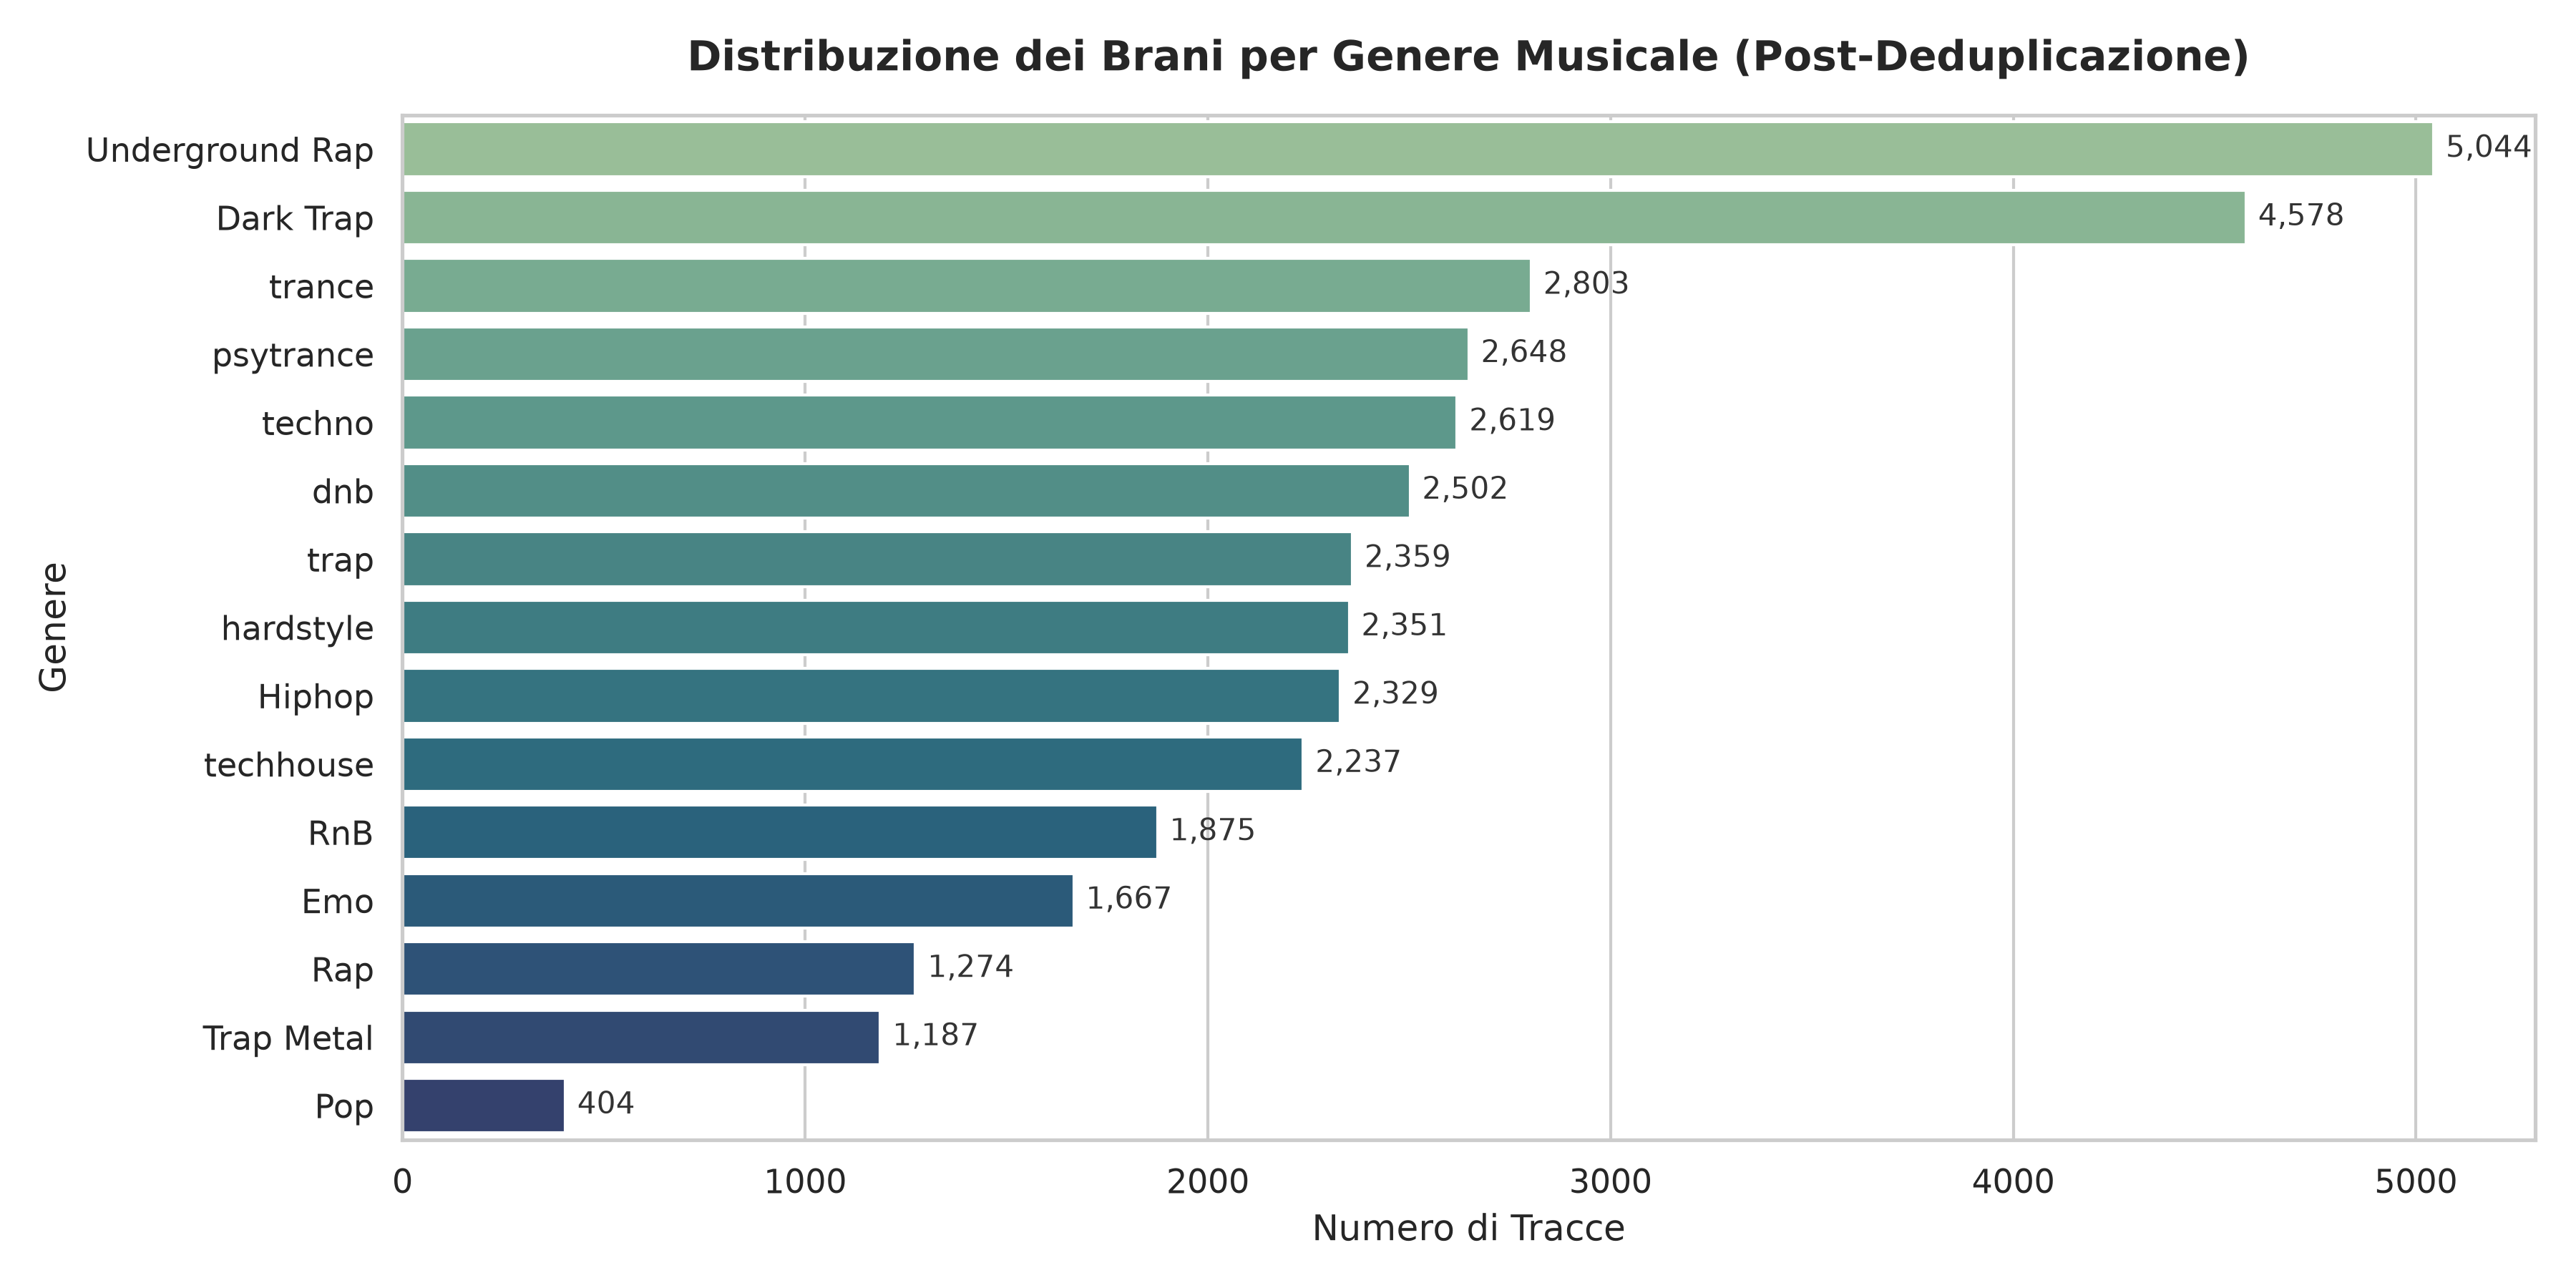
\includegraphics[width=0.88\textwidth]{figures/fig01_distribuzione_generi.png}
    \caption{Distribuzione delle frequenze dei 15 generi musicali post-deduplicazione.}
    \label{fig:distribuzione_generi}
\end{figure}

\subsubsection{Distribuzione delle feature continue}
In Figura \ref{fig:audio_features_hist} vengono mostrati gli istogrammi arricchiti con curve di densità (KDE) per le caratteristiche continue:
\begin{itemize}
    \item \texttt{danceability}: Presenta una distribuzione simmetrica centrata tra 0.65 e 0.70.
    \item \texttt{energy} e \texttt{loudness}: Sono fortemente asimmetriche a sinistra, evidenziando che la produzione discografica moderna privilegia dinamiche compresse e volumi elevati (-8 dB a -4 dB).
    \item \texttt{acousticness}: Mostra un forte picco vicino a zero, confermando che la quasi totalità delle tracce include produzione elettronica.
    \item \texttt{speechiness}: Mostra una struttura bimodale, con un picco sotto 0.1 per musica melodica e un secondo cluster sopra 0.25 tipico di Rap e Trap.
\end{itemize}

\begin{figure}[H]
    \centering
    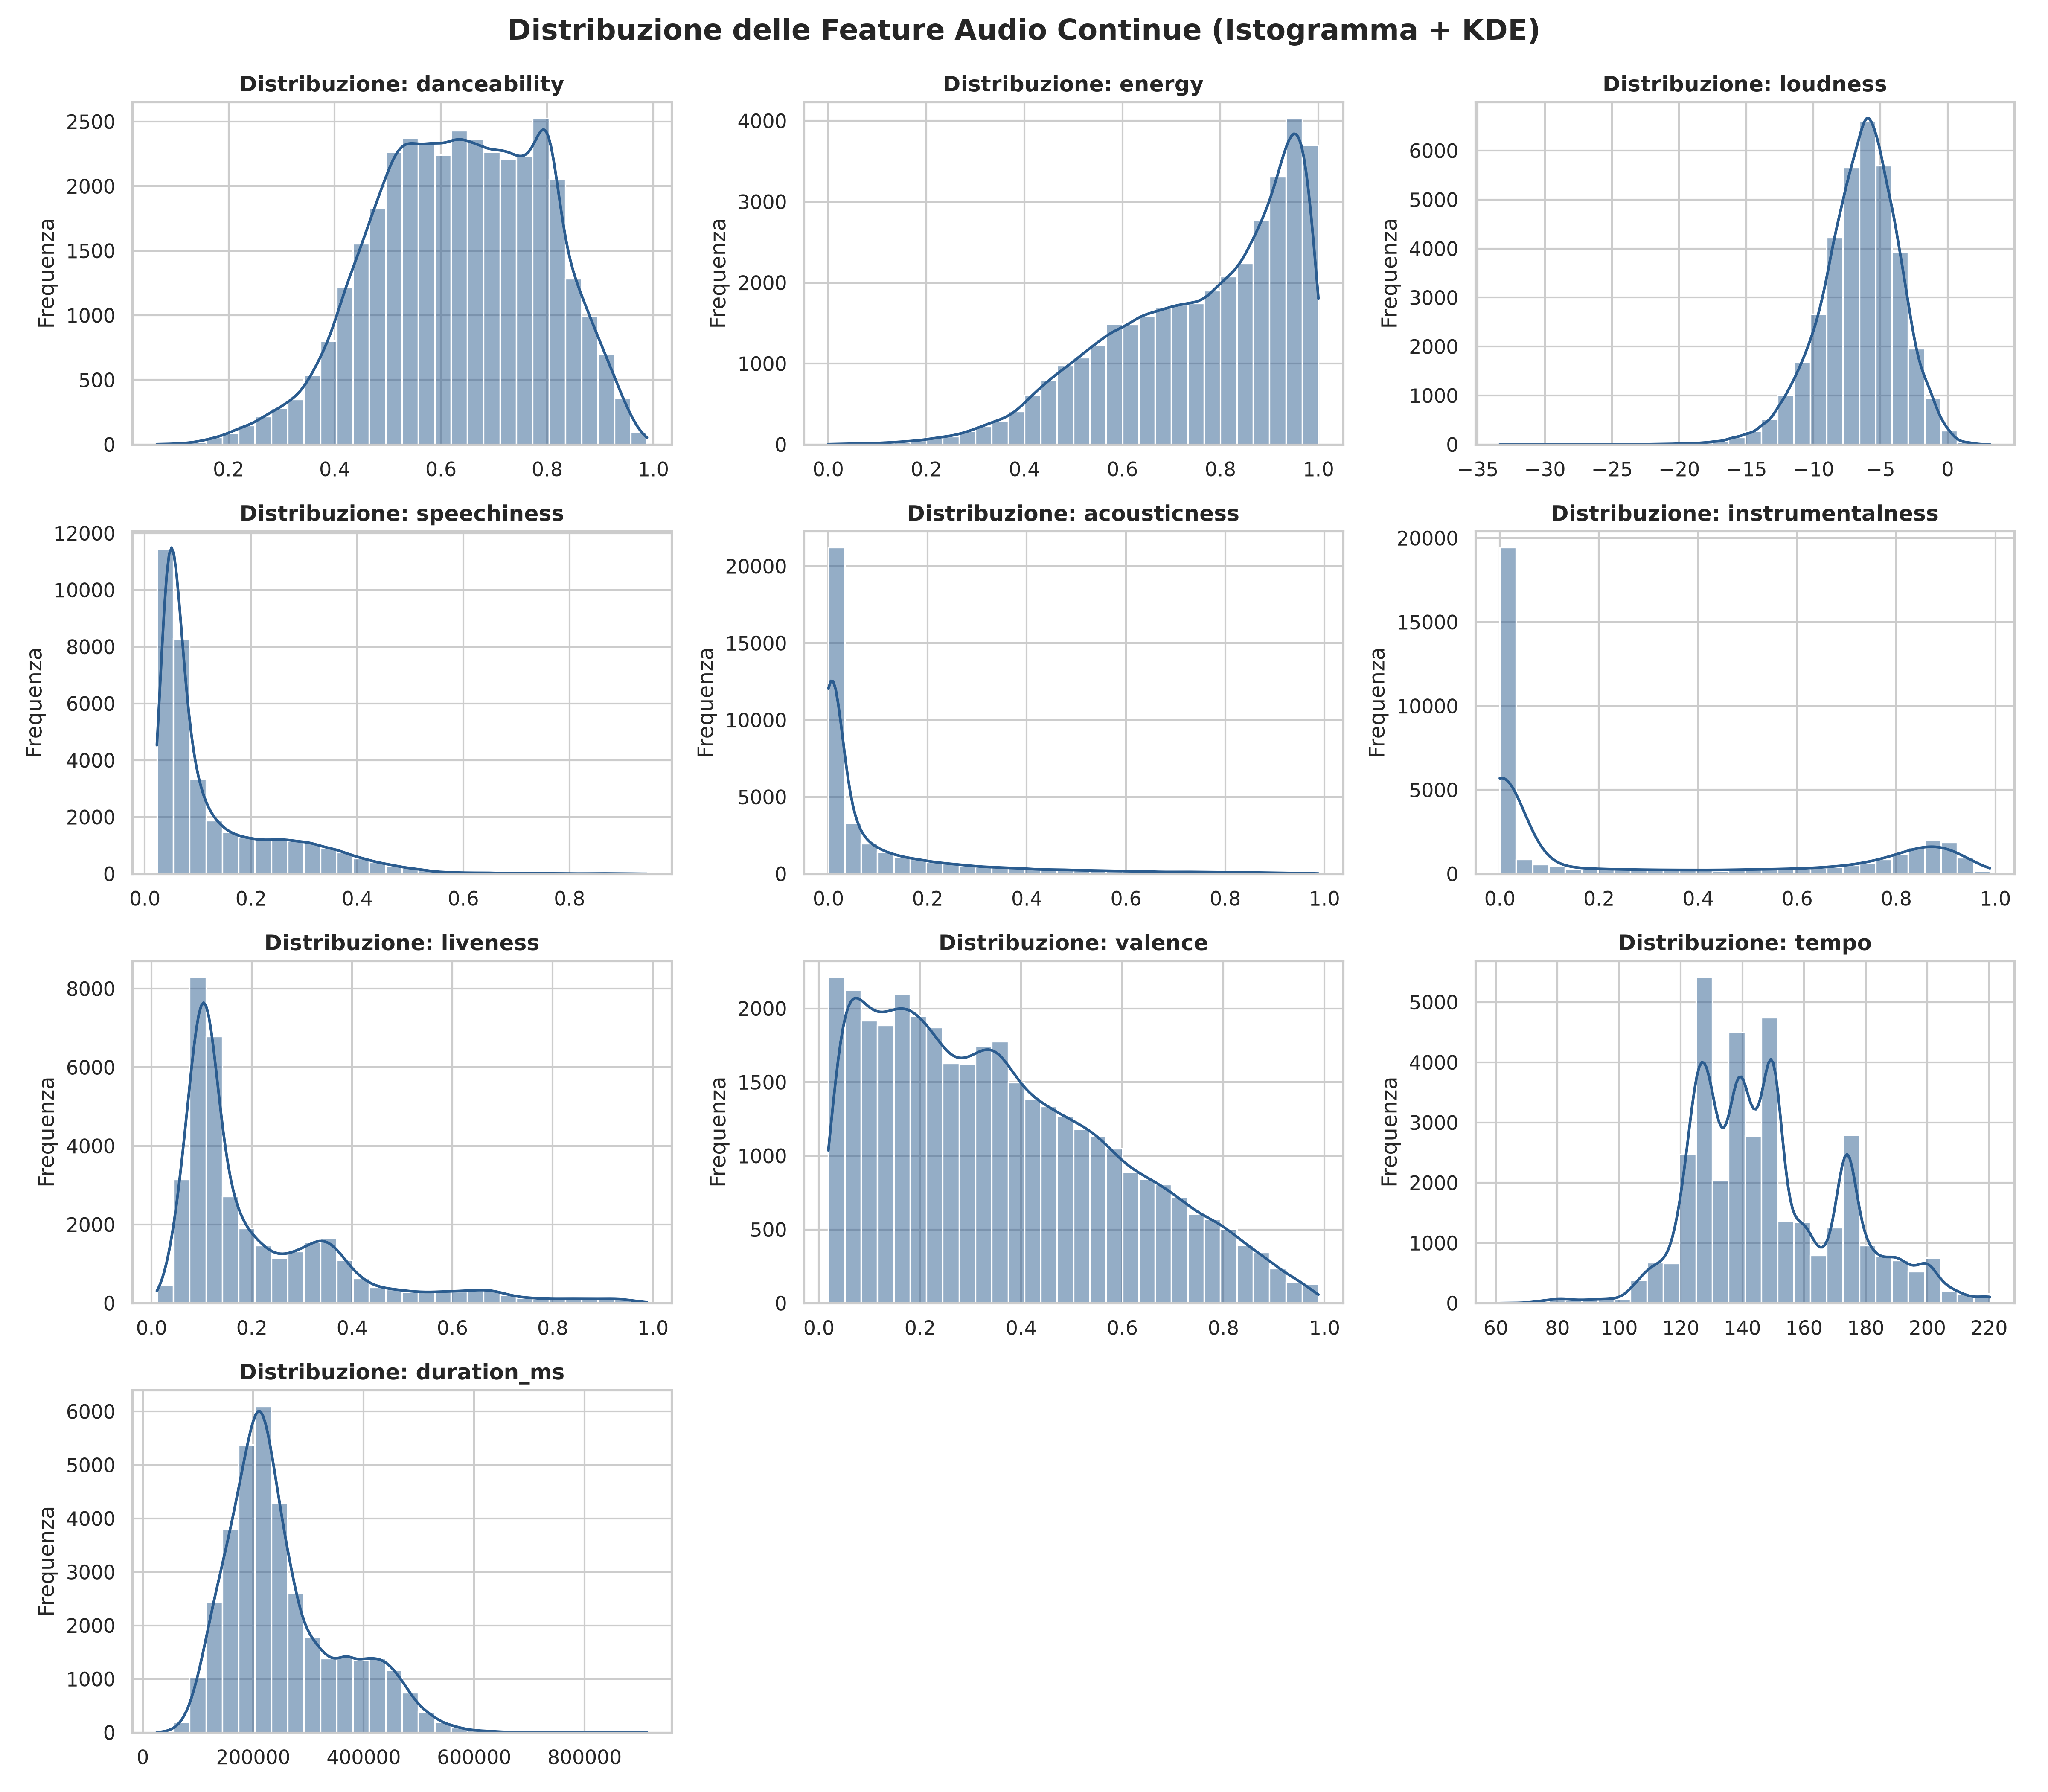
\includegraphics[width=0.95\textwidth]{figures/fig02_audio_features_hist_kde.png}
    \caption{Distribuzione delle feature audio continue (istogrammi e curve di densità KDE).}
    \label{fig:audio_features_hist}
\end{figure}

\subsubsection{Distribuzione delle variabili discrete}
In Figura \ref{fig:discrete_features} viene rappresentata la distribuzione della tonalità (\texttt{key}), della modalità (\texttt{mode}) e del metro (\texttt{time\_signature}). Si nota una prevalenza netta della misura standard in 4/4 e una leggera predominanza della modalità maggiore (\texttt{mode} = 1).

\begin{figure}[H]
    \centering
    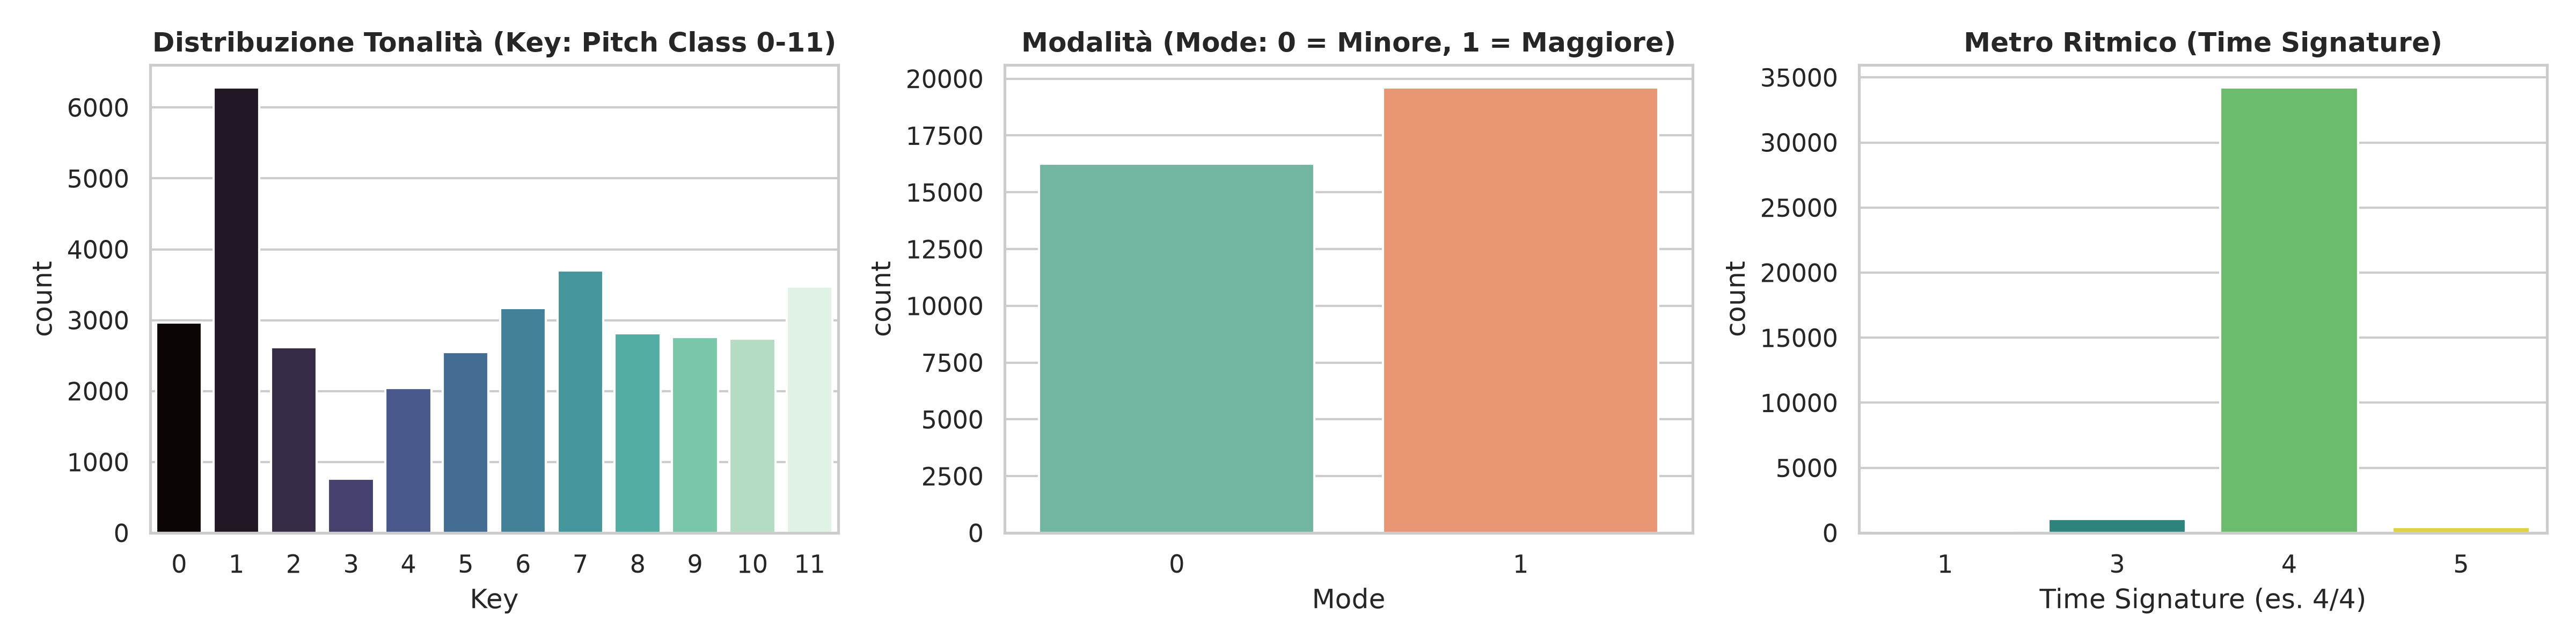
\includegraphics[width=0.95\textwidth]{figures/fig03_discrete_features.png}
    \caption{Distribuzione delle variabili musicali discrete: Tonalità, Modalità e Metro.}
    \label{fig:discrete_features}
\end{figure}

\subsubsection{Matrice di correlazione}
È stata calcolata la matrice di correlazione lineare di Pearson tra le feature audio, visualizzata tramite heatmap in Figura \ref{fig:matrice_corr_iniziale}.
Dall'analisi emergono forti correlazioni tra grandezze fisiche:
\begin{itemize}
    \item Forte correlazione positiva tra \texttt{energy} e \texttt{loudness} ($r \approx 0.70$).
    \item Forte correlazione negativa tra \texttt{energy} e \texttt{acousticness} ($r \approx -0.49$).
    \item Correlazione positiva moderata tra \texttt{valence} (positività emotiva) e \texttt{danceability}.
\end{itemize}

\begin{figure}[H]
    \centering
    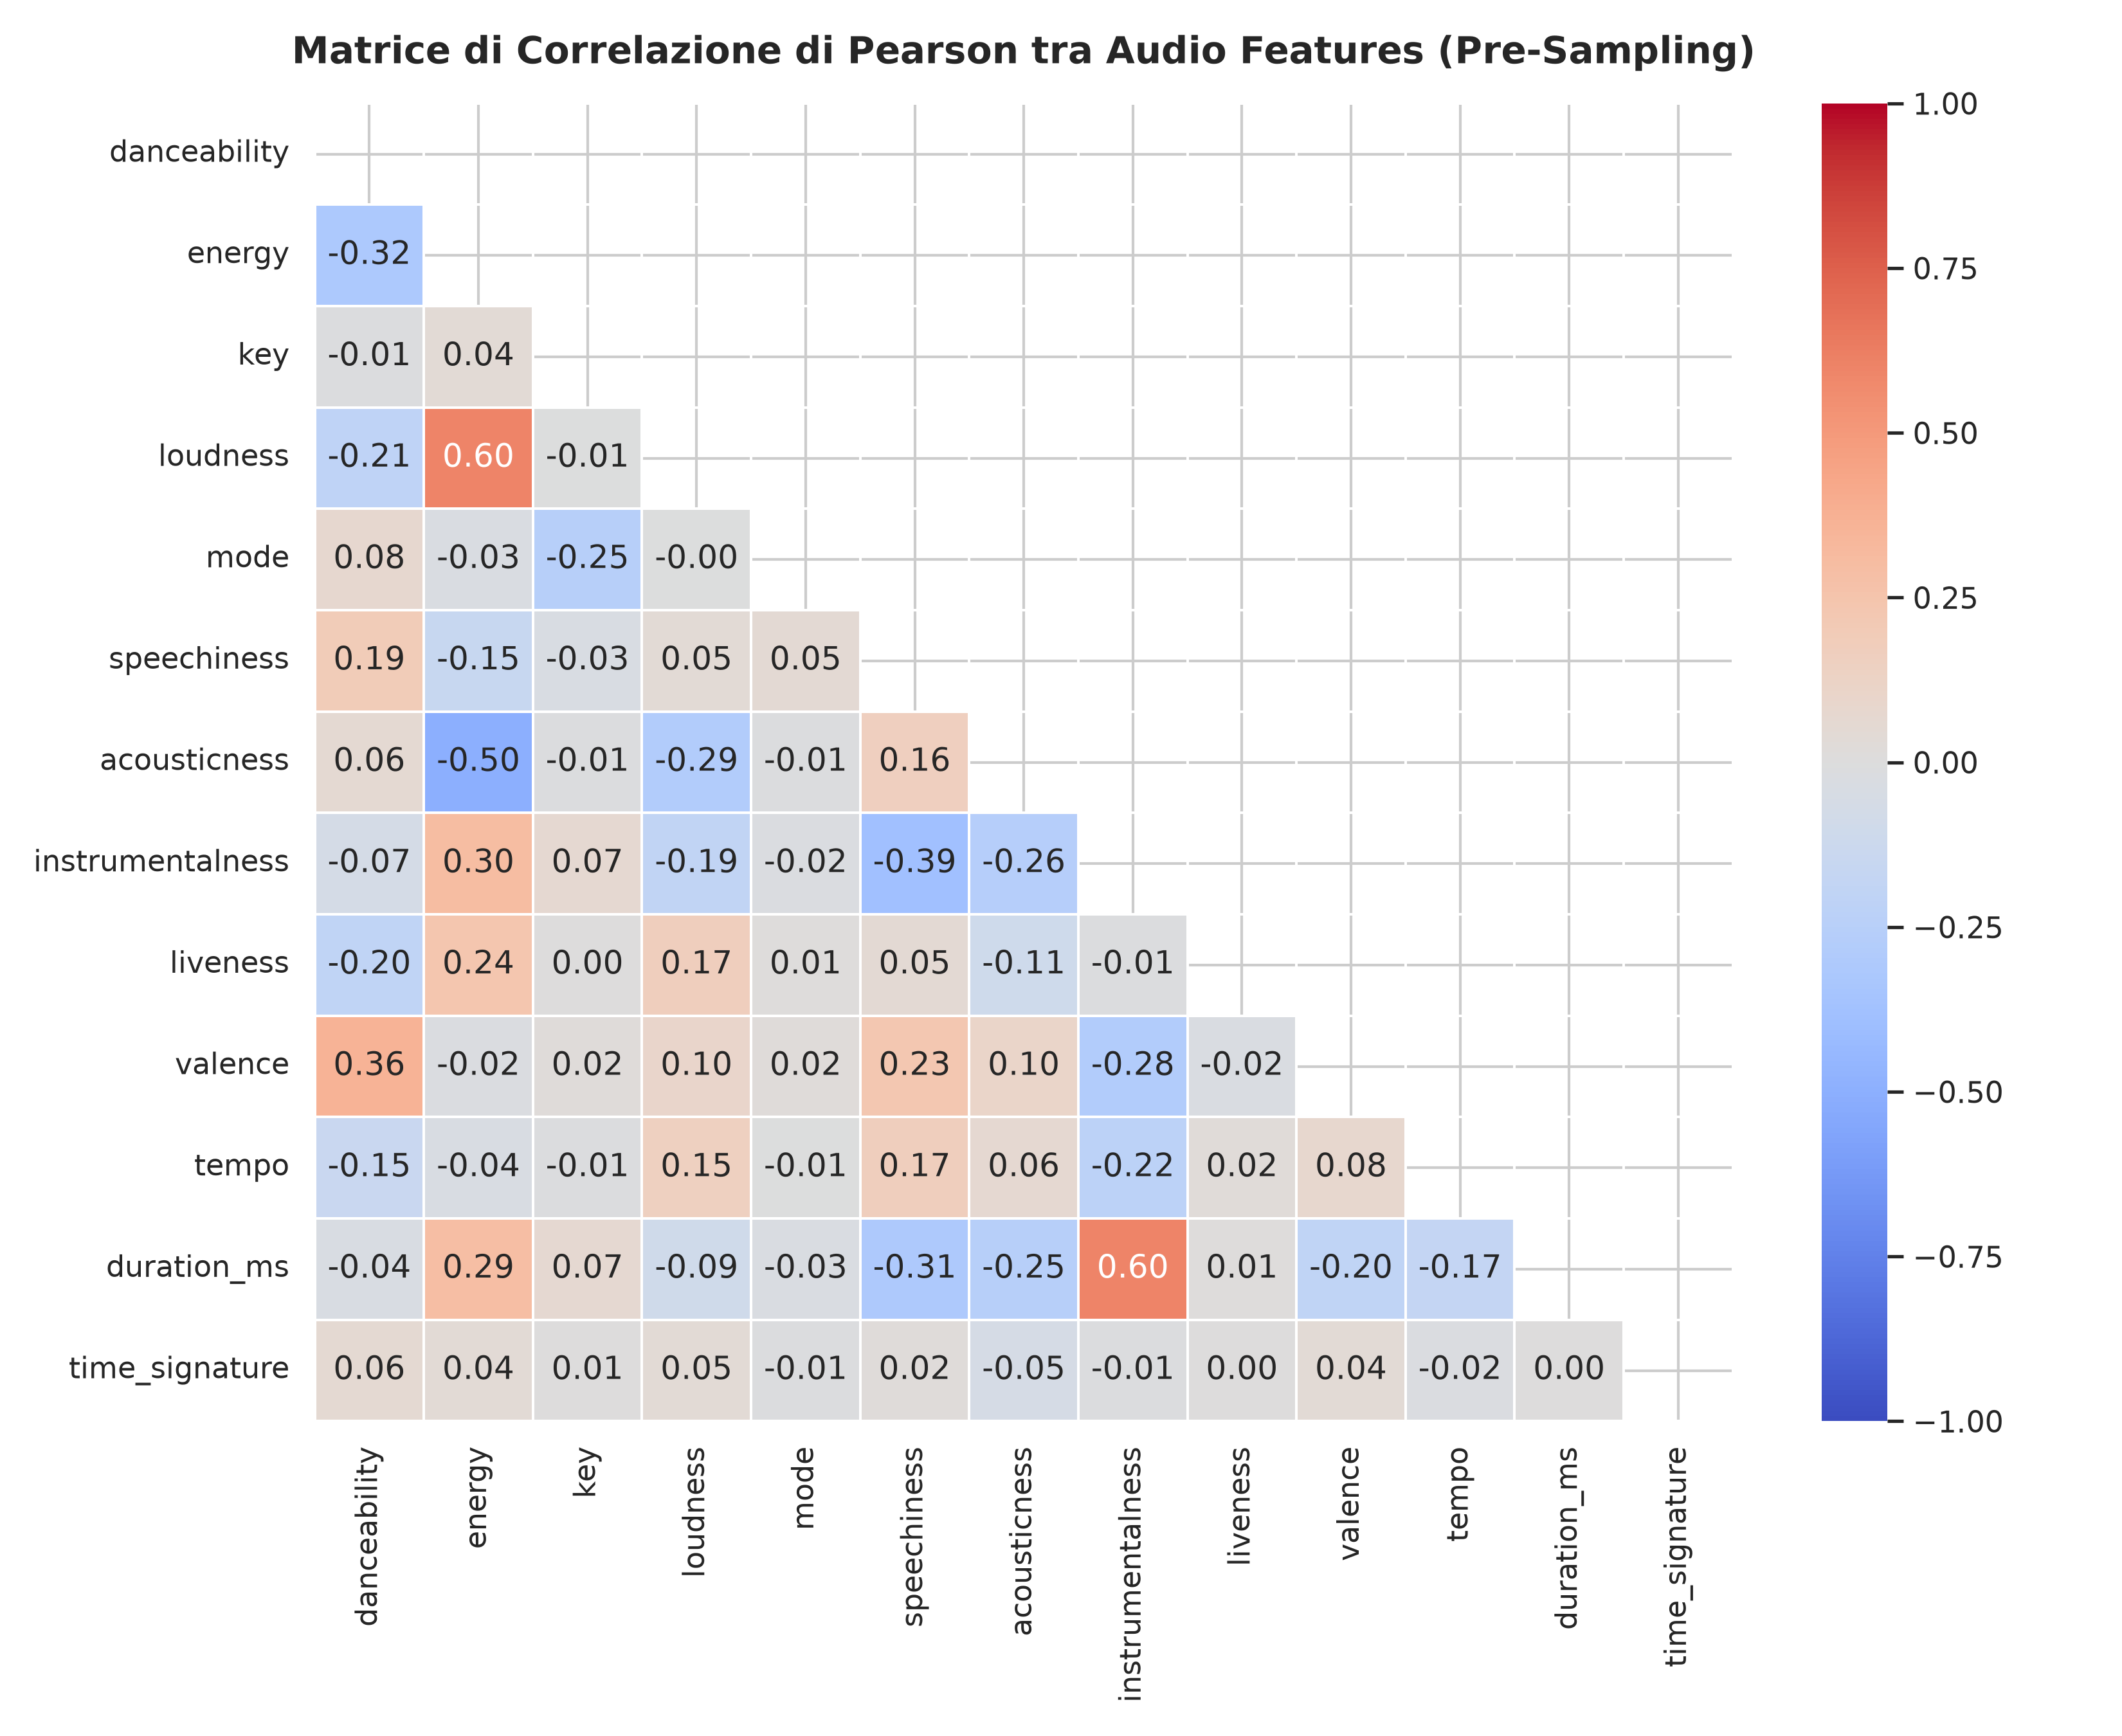
\includegraphics[width=0.80\textwidth]{figures/fig04_matrice_correlazione_iniziale.png}
    \caption{Matrice di correlazione di Pearson tra le feature audio prima delle operazioni di sampling.}
    \label{fig:matrice_corr_iniziale}
\end{figure}

\newpage
% =========================================================================
% CAPITOLO 3: CLASSIFICAZIONE
% =========================================================================
\section{Spotify tracks analysis: Classificazione}

La classificazione supervisionata è stata condotta con l'obiettivo di sviluppare modelli predittivi capaci di assegnare la corretta etichetta di genere musicale a ciascuna traccia sulla base esclusiva dei suoi parametri sonori.

\subsection{Preprocessing del Dataset}
Per preparare correttamente i dati, il dataset di 35.877 brani è stato suddiviso in Training Set (80\%, 28.701 campioni) e Test Set (20\%, 7.176 campioni) mediante stratificazione rispetto alle classi target.

Per evitare fenomeni di \textit{data leakage}, la standardizzazione tramite \texttt{StandardScaler} è stata calcolata (\textit{fit}) unicamente sul training set ed estesa (\textit{transform}) sul test set:
\begin{equation}
z = \frac{x - \mu_{train}}{\sigma_{train}}
\end{equation}

\subsubsection{Oversampling con SMOTE e Undersampling}
A causa del forte sbilanciamento (le classi variano da circa 400 a oltre 5.000 campioni), un classificatore standard tenderebbe a collassare sulle classi dominanti. È stata adottata una strategia combinata applicata \textbf{esclusivamente al training set}:
\begin{itemize}
    \item \textbf{SMOTE (Synthetic Minority Oversampling Technique):} Ha incrementato il numero di campioni per le classi minoritarie (\textit{Pop, Trap Metal, Rap, Emo, RnB}) generando campioni sintetici mediante interpolazione lineare nello spazio delle feature.
    \item \textbf{Undersampling Controllato:} Ha ridotto i campioni delle classi maggioritarie (\textit{Underground Rap, Dark Trap}).
\end{itemize}

\subsubsection{Dataset Finale}
Dopo l'applicazione di entrambe le tecniche, il training set bilanciato presenta esattamente \textbf{2.000 campioni per ciascuna delle 15 classi} (30.000 osservazioni complessive). Il test set di 7.176 osservazioni è stato invece preservato nella sua distribuzione reale originale per una stima priva di bias. In Figura \ref{fig:distribuzione_sampling} viene mostrato il confronto tra le distribuzioni prima e dopo l'intervento di bilanciamento.

\begin{figure}[H]
    \centering
    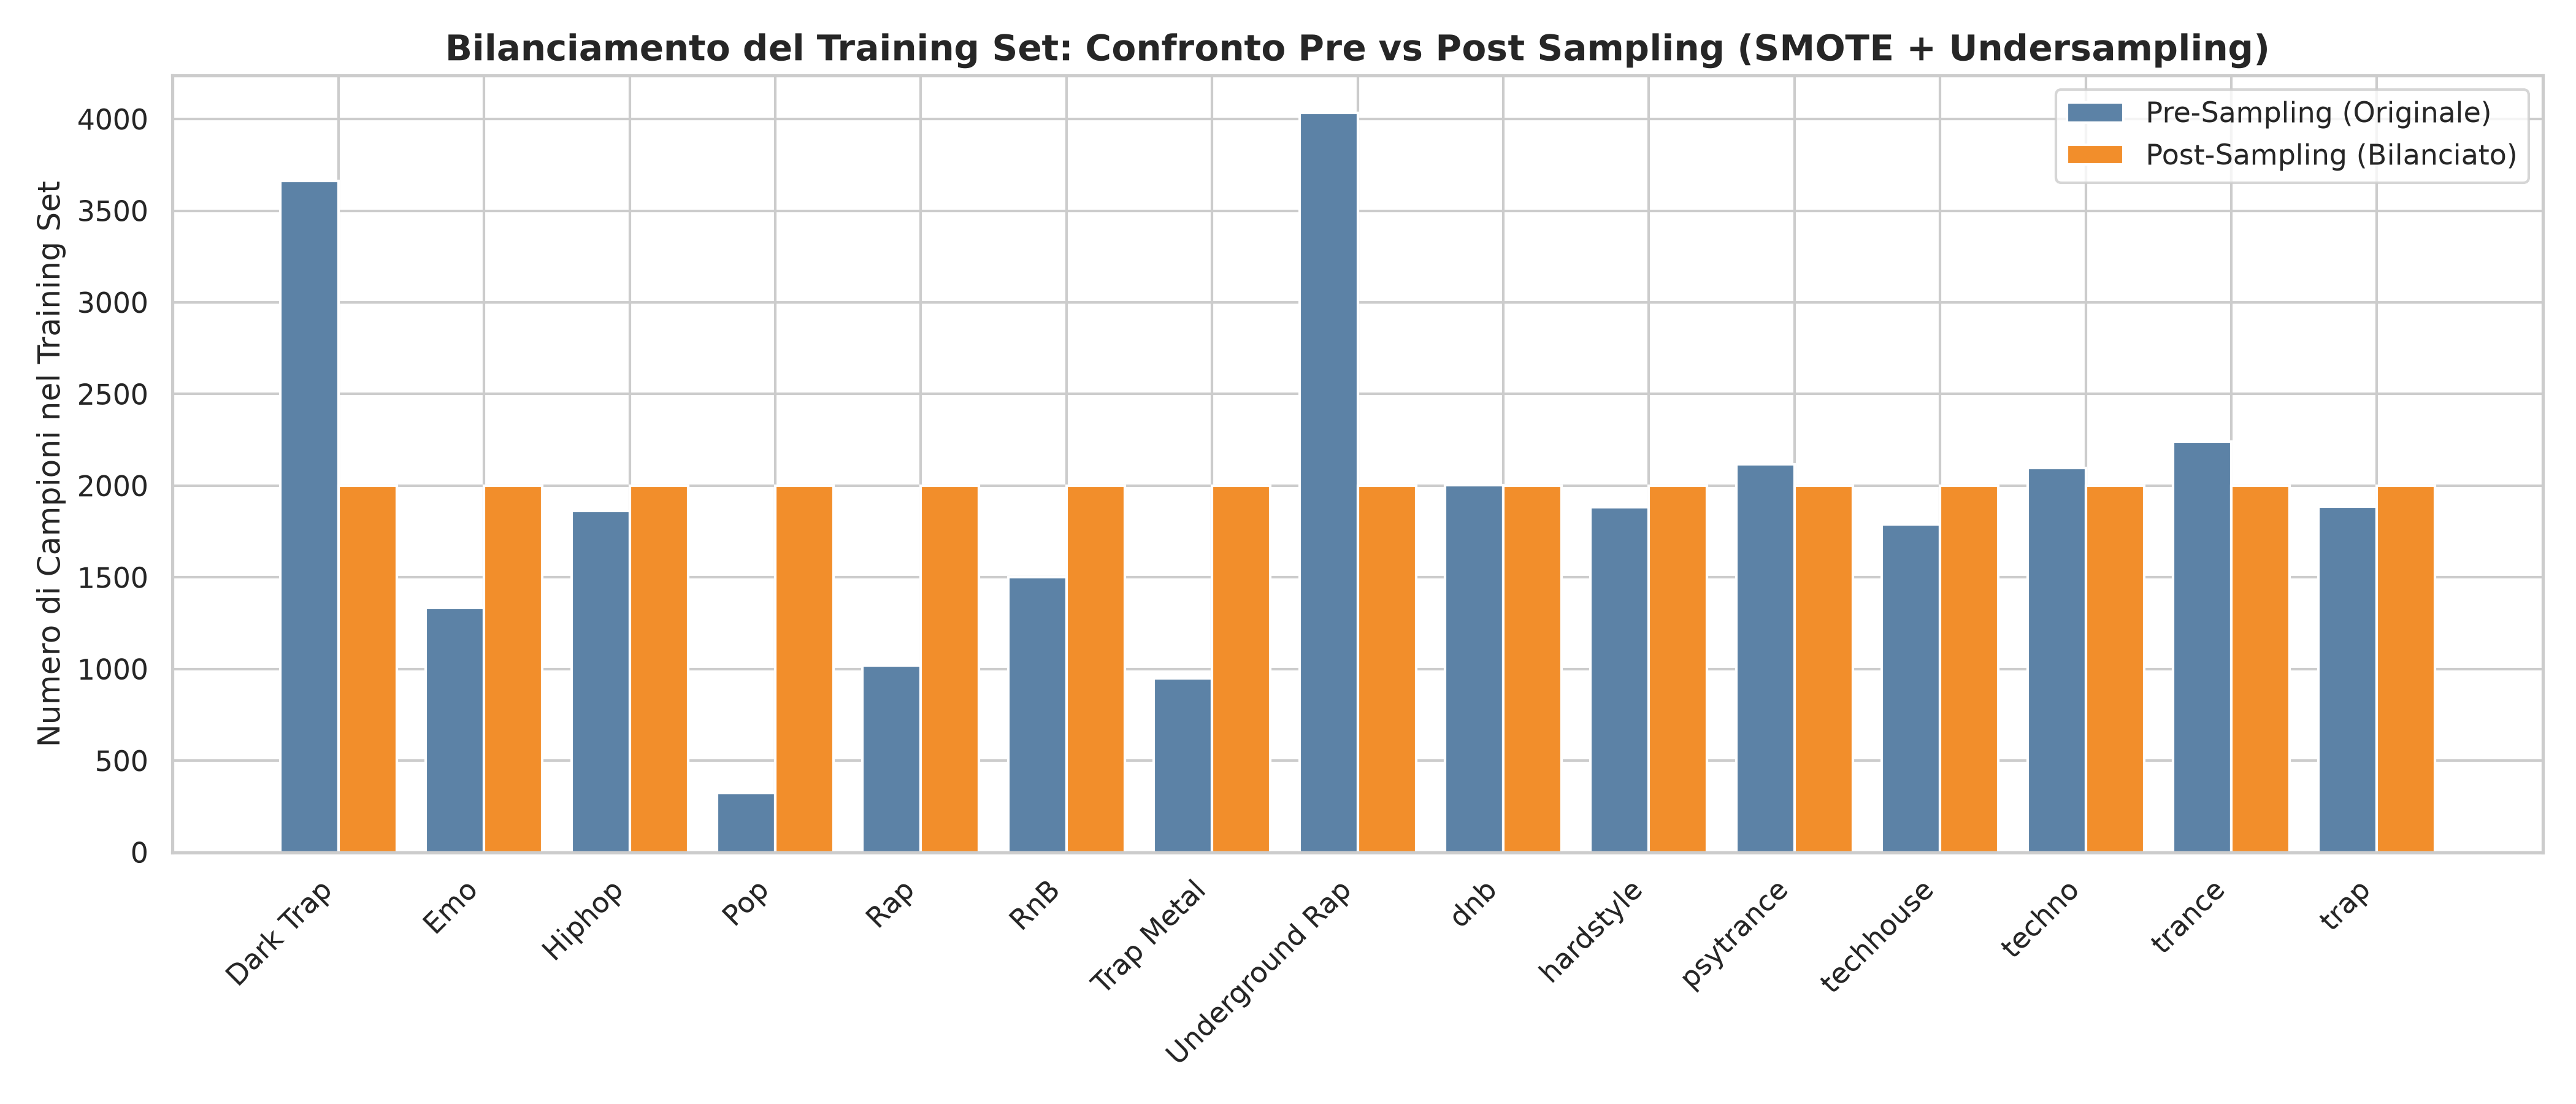
\includegraphics[width=0.90\textwidth]{figures/fig05_distribuzione_sampling.png}
    \caption{Distribuzione dei generi nel Training Set prima e dopo il campionamento (SMOTE + Undersampling).}
    \label{fig:distribuzione_sampling}
\end{figure}

\subsubsection{Analisi della distribuzione degli attributi}
Al termine delle operazioni di campionamento è stata ricalcolata la matrice di correlazione sul dataset bilanciato (Figura \ref{fig:matrice_corr_post}). Il confronto con la matrice originale (Figura \ref{fig:matrice_corr_iniziale}) attesta che la struttura relazionale dei dati è rimasta perfettamente coerente, confermando che SMOTE non ha introdotto artefatti o distorsioni spaziali.

\begin{figure}[H]
    \centering
    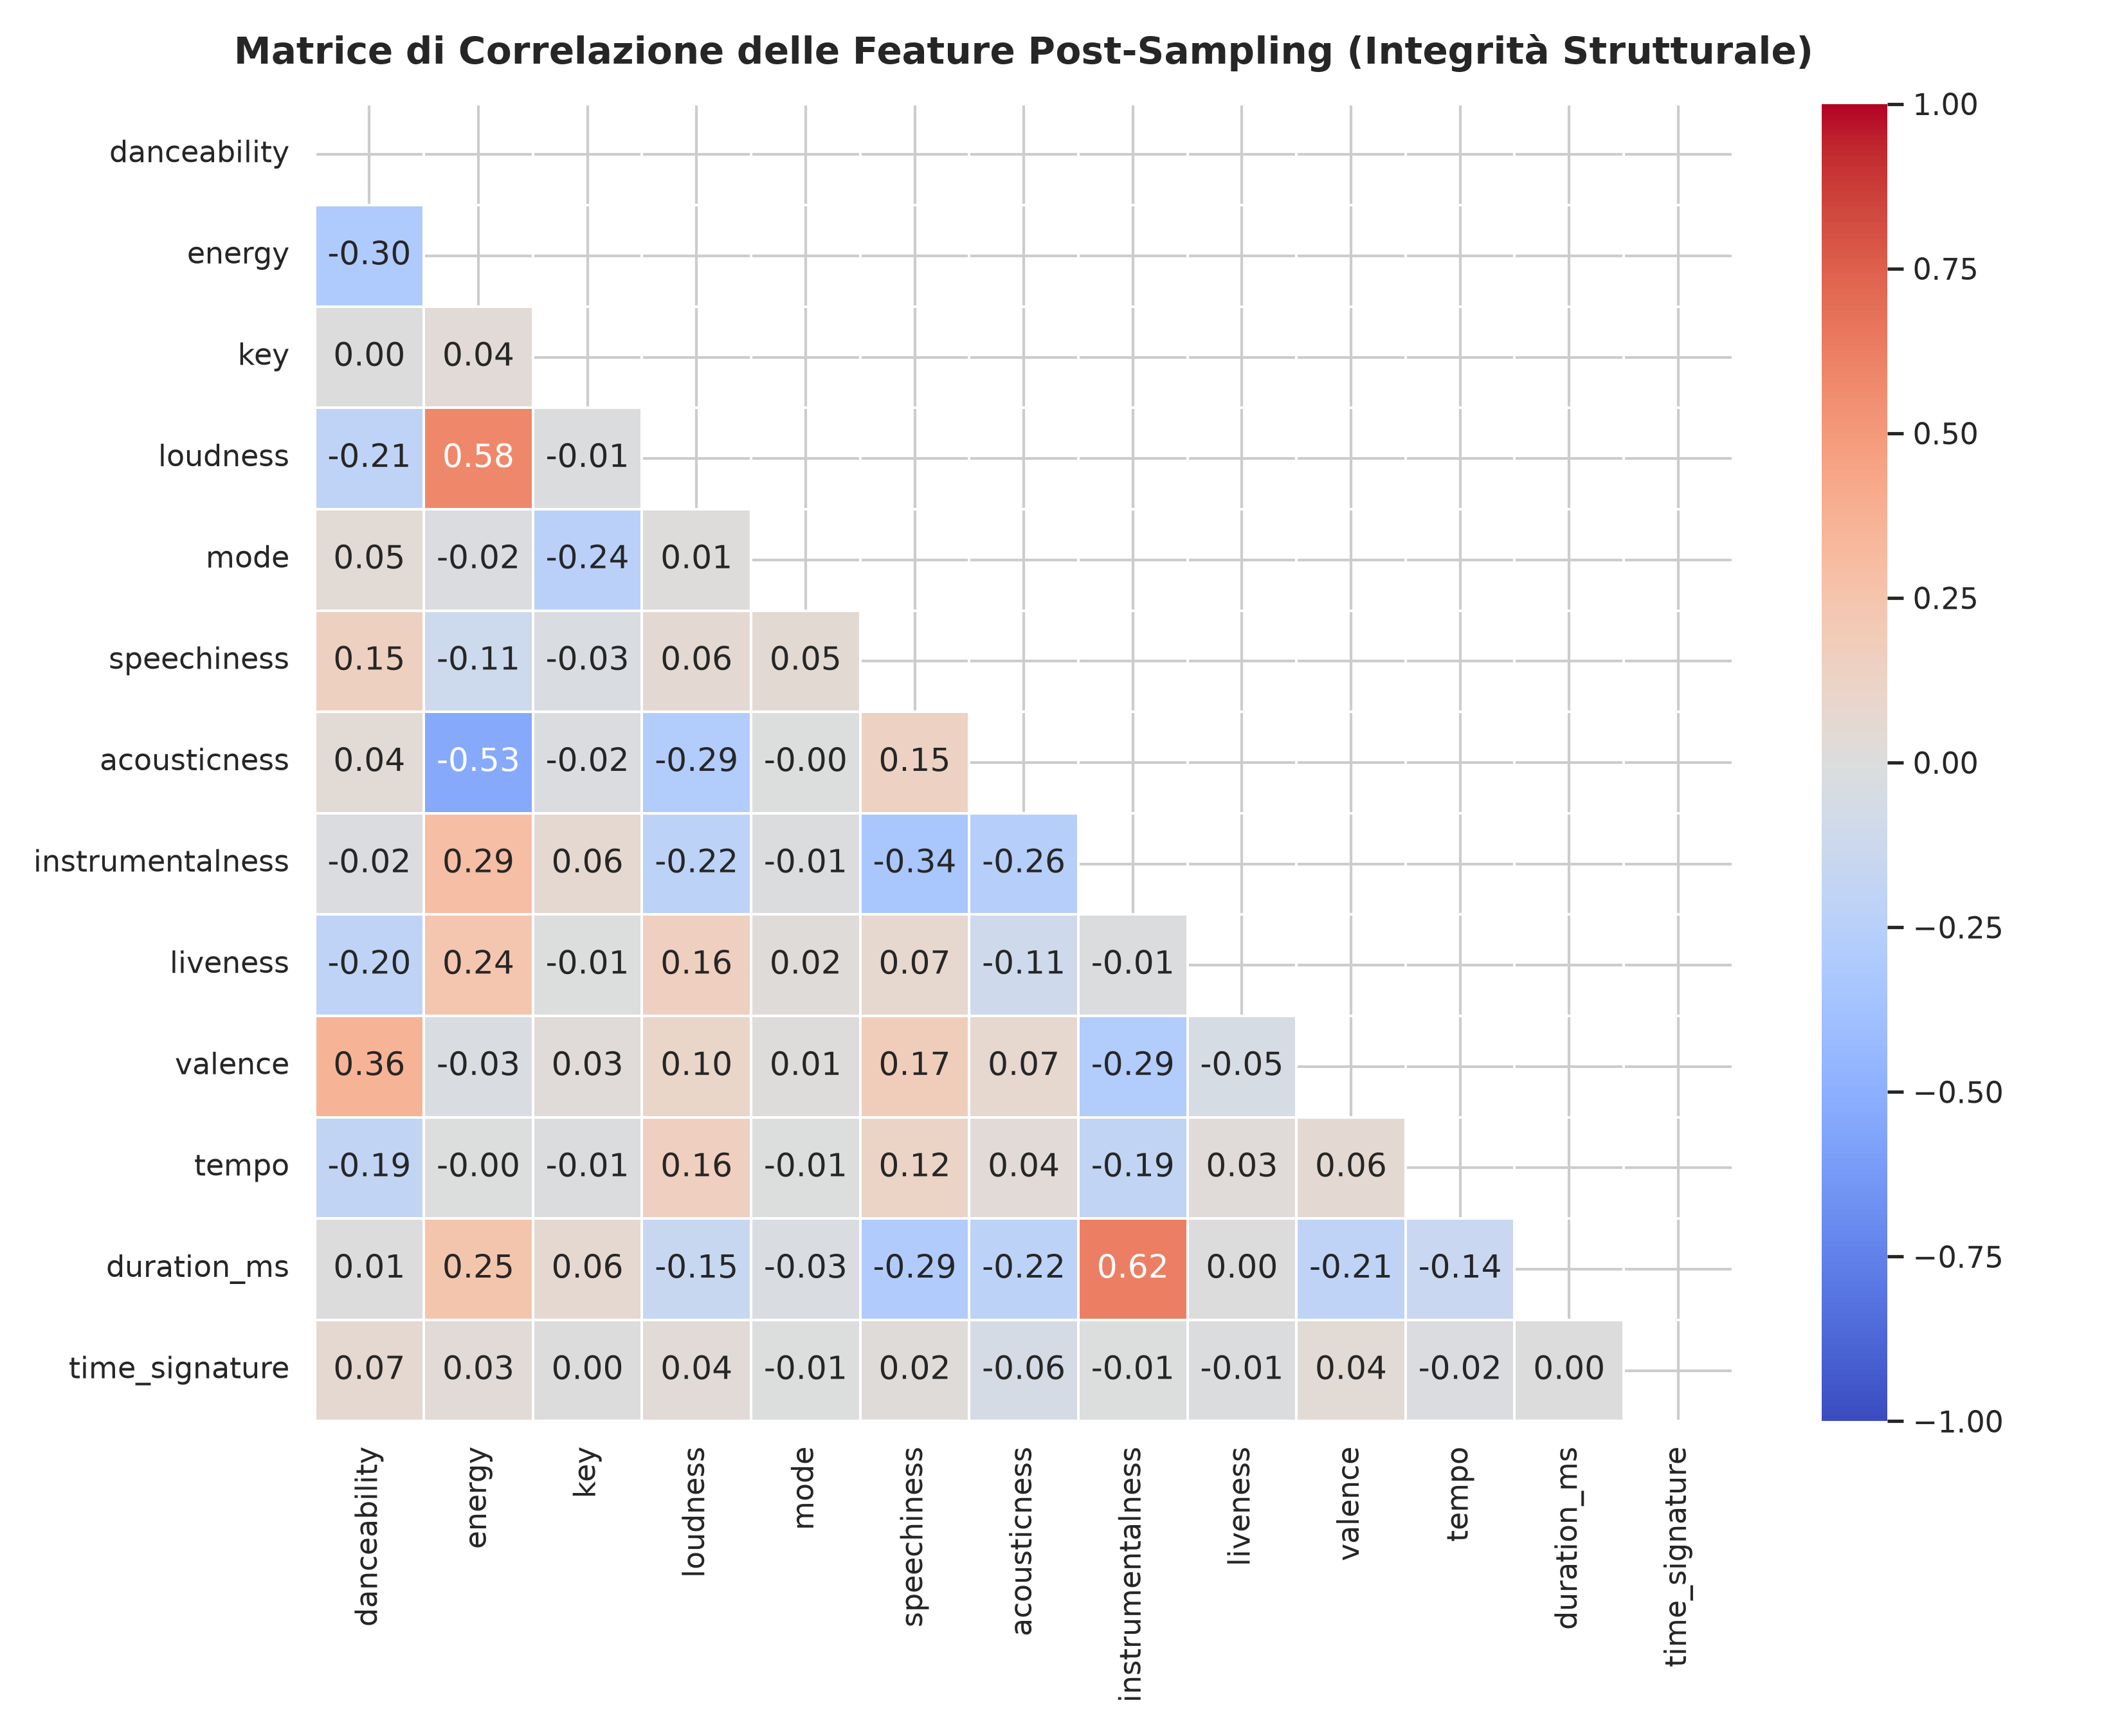
\includegraphics[width=0.80\textwidth]{figures/fig06_matrice_correlazione_post_sampling.png}
    \caption{Matrice di correlazione delle feature audio calcolata dopo il processo di bilanciamento.}
    \label{fig:matrice_corr_post}
\end{figure}

\subsection{Processo di Classificazione e Confronto Modelli}
Il processo di classificazione ha previsto il confronto su un banco di prova uniforme di 8 differenti algoritmi di apprendimento automatico:
\begin{enumerate}
    \item \textbf{Logistic Regression:} Baseline lineare con penalità $L_2$ e formulazione multinomiale.
    \item \textbf{Decision Tree:} Albero decisionale singolo regolarizzato con profondità massima.
    \item \textbf{Random Forest:} Ensemble bagging di 100 alberi decisionali indipendenti.
    \item \textbf{K-Nearest Neighbors (KNN):} Classificatore a vicini con metrica euclidea ($k=9$).
    \item \textbf{Gaussian Naive Bayes:} Modello probabilistico basato su stima delle densità gaussiane.
    \item \textbf{AdaBoost Classifier:} Algoritmo di boosting basato sulla riponderazione iterativa dei residui.
    \item \textbf{Gradient Boosting Classifier:} Boosting sequenziale basato sulla discesa del gradiente.
    \item \textbf{XGBoost (Extreme Gradient Boosting):} Implementazione efficiente di gradient boosted trees con regolarizzazione nativa.
\end{enumerate}

I risultati ottenuti valutando i modelli sul Test Set (7.176 brani) sono riportati in Tabella \ref{tab:risultati_modelli} e illustrati graficamente in Figura \ref{fig:confronto_modelli}.

\begin{table}[H]
\centering
\caption{Confronto delle performance dei modelli sul Test Set indipendente.}
\label{tab:risultati_modelli}
\begin{tabular}{lcccc}
\toprule
\textbf{Modello} & \textbf{Accuratezza} & \textbf{Weighted F1} & \textbf{Macro F1} & \textbf{Tempo Addestr. (s)} \\
\midrule
XGBoost & 0.6745 & 0.6763 & 0.6480 & 1.91 \\
Random Forest & 0.6734 & 0.6726 & 0.6498 & 1.04 \\
Gradient Boosting & 0.6630 & 0.6634 & 0.6397 & 101.16 \\
Decision Tree & 0.5916 & 0.5960 & 0.5734 & 0.39 \\
Logistic Regression & 0.5516 & 0.5560 & 0.5279 & 0.86 \\
K-Nearest Neighbors & 0.5394 & 0.5425 & 0.5213 & 1.25 \\
Gaussian Naive Bayes & 0.5332 & 0.5364 & 0.5198 & 0.02 \\
AdaBoost & 0.3686 & 0.3513 & 0.3261 & 2.12 \\
\bottomrule
\end{tabular}
\end{table}

\begin{figure}[H]
    \centering
    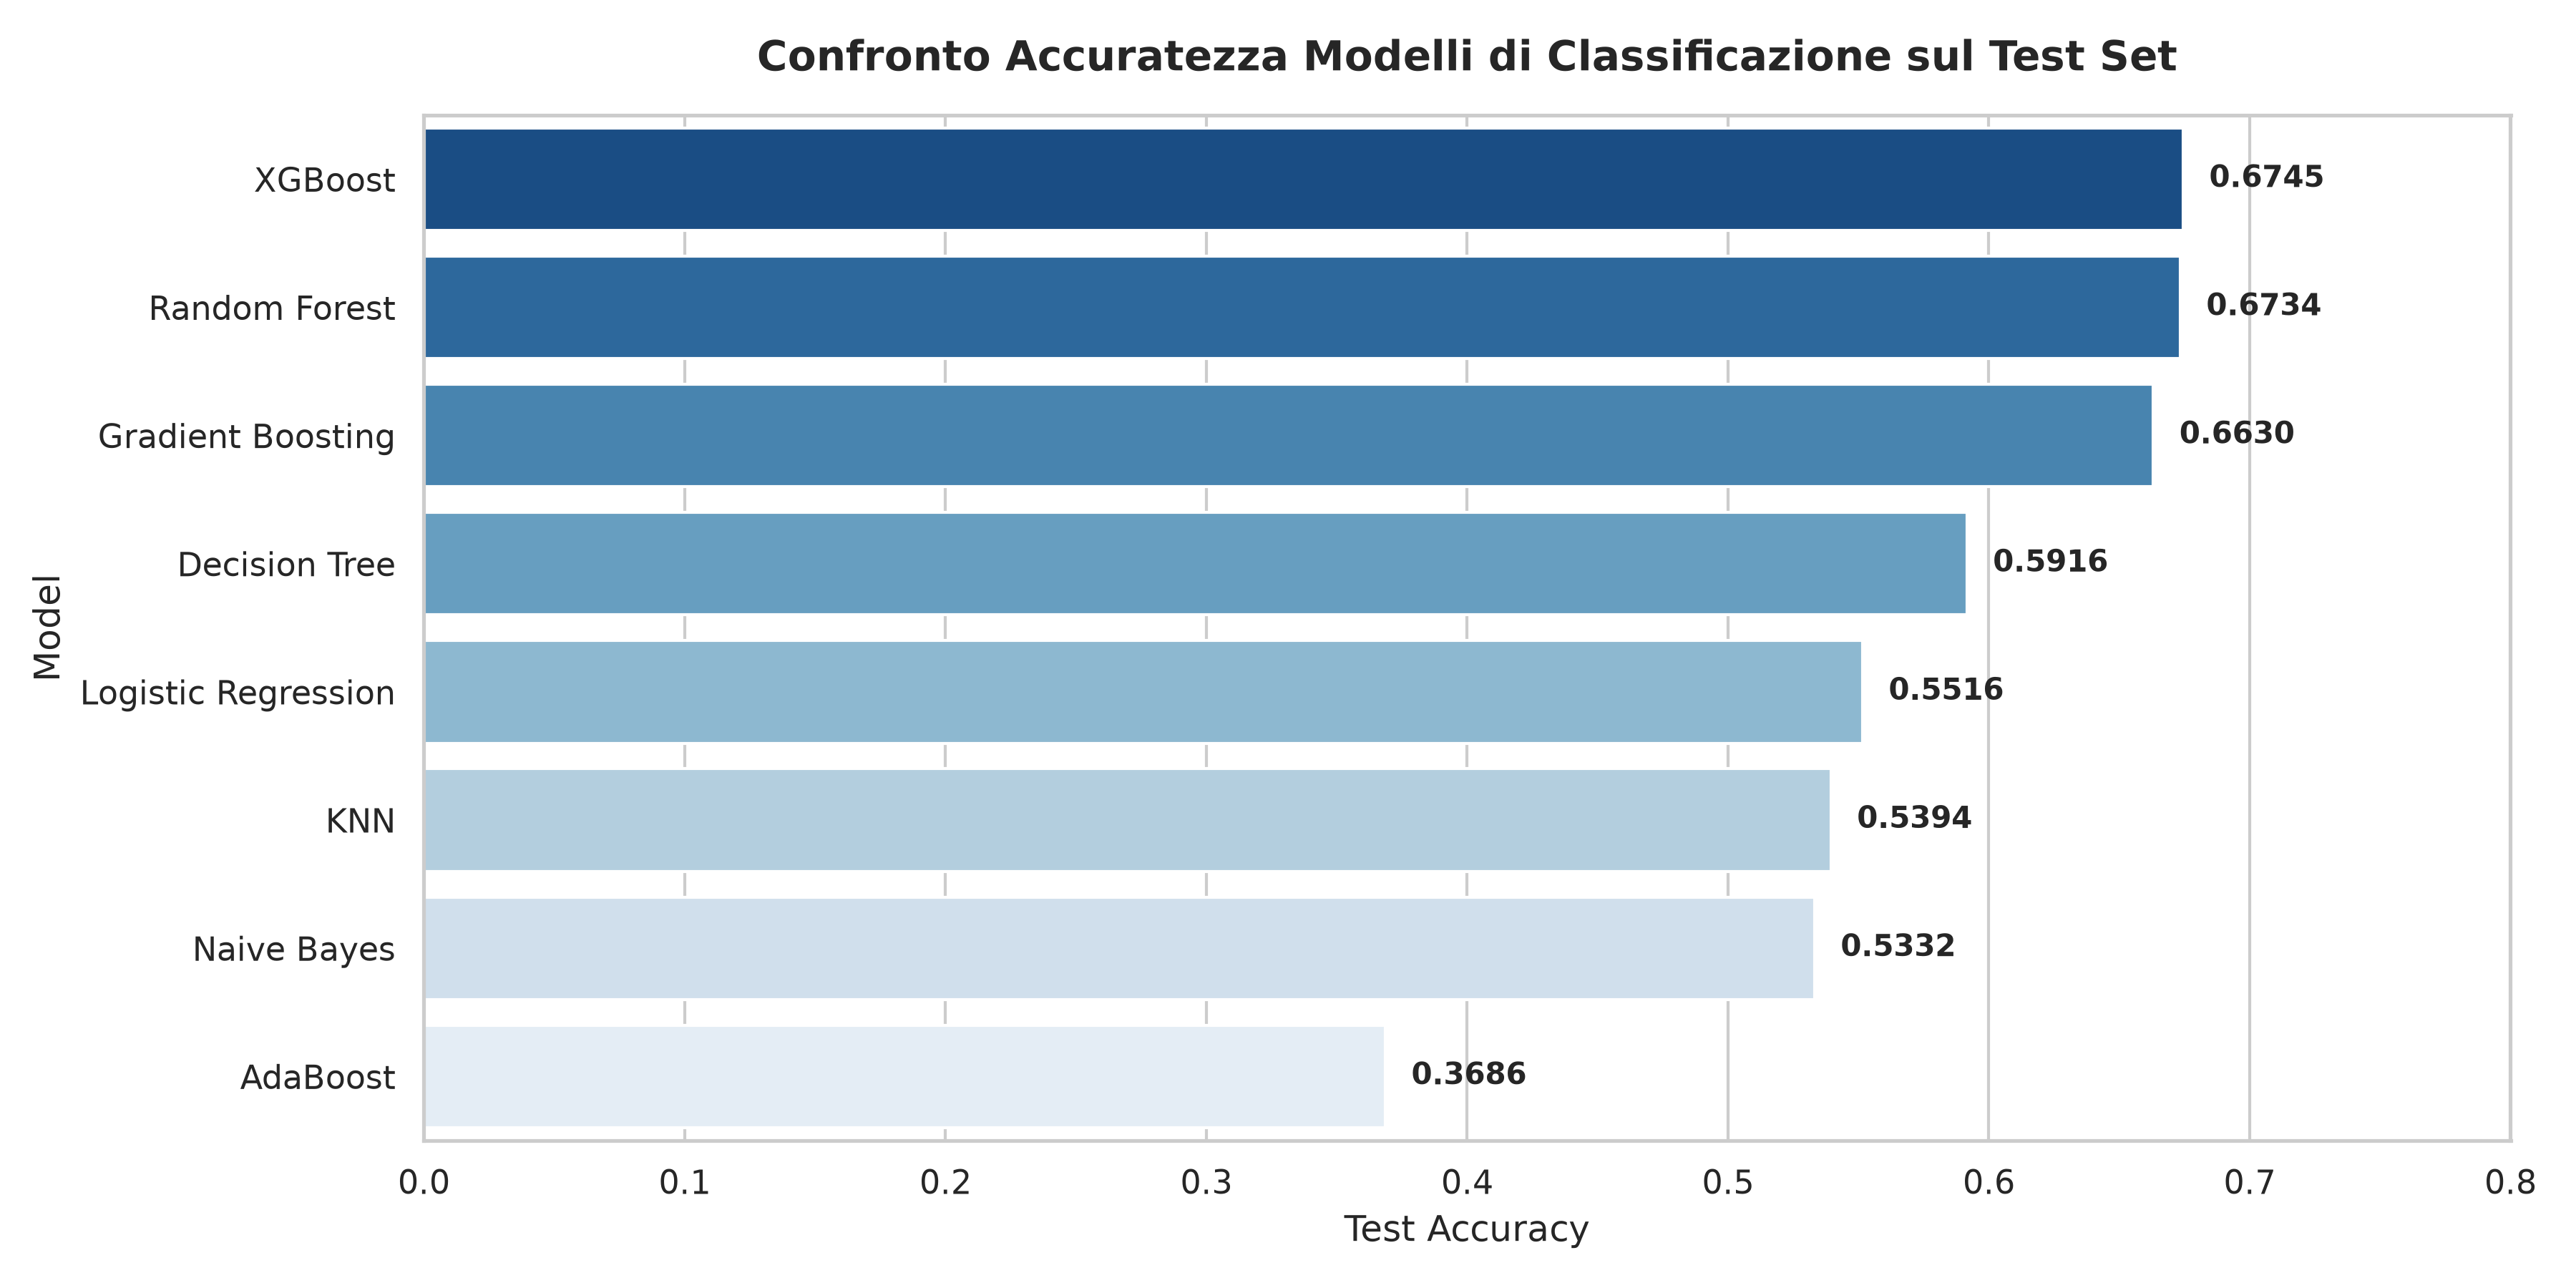
\includegraphics[width=0.88\textwidth]{figures/fig07_confronto_modelli_baseline.png}
    \caption{Confronto dell'accuratezza media ottenuta dai diversi algoritmi sul Test Set.}
    \label{fig:confronto_modelli}
\end{figure}

\subsection{Ensemble Learning}
Per massimizzare la capacità di generalizzazione e ridurre la varianza residua, sono state adottate due tecniche di Ensemble Learning avanzate:
\begin{itemize}
    \item \textbf{Voting Classifier (Soft Voting):} Combina le stime di probabilità a posteriori dei tre classificatori con le migliori prestazioni singole (\textit{XGBoost, Random Forest e Gradient Boosting}). La previsione finale massimizza la probabilità media:
    \begin{equation}
    \hat{y} = \arg\max_{c} \frac{1}{M} \sum_{m=1}^M P_m(y=c \mid x)
    \end{equation}
    Questo modello ottiene un'accuratezza sul test set del \textbf{68.00\%} e un Weighted F1 di \textbf{0.6810}.
    \item \textbf{Stacking Classifier:} Utilizza un'architettura a due livelli: i modelli di base (\textit{XGBoost, Random Forest e Logistic Regression}) generano previsioni out-of-fold tramite cross-validation a 3-fold, che fungono da input per un meta-modello di Regressione Logistica. Questo approccio raggiunge un'accuratezza del \textbf{68.90\%} e un Weighted F1 di \textbf{0.6890}, costituendo il miglior risultato complessivo dell'analisi.
\end{itemize}

\subsection{Diagnostica e Commento ai Risultati}
Le prestazioni dell'ensemble finale sono state analizzate approfonditamente attraverso una serie completa di strumenti diagnostici.

\subsubsection{Classification Report e Matrice di Confusione}
La Figura \ref{fig:confusion_matrix} illustra la matrice di confusione normalizzata, mentre la Figura \ref{fig:classification_report} riporta l'heatmap del Classification Report (Precision, Recall ed F1-Score per ogni genere).
L'analisi rivela un comportamento sonoro altamente coerente:
\begin{itemize}
    \item Generi con forte identità timbrica e ritmica (\textit{dnb}, \textit{hardstyle}, \textit{psytrance}, \textit{techno}) ottengono un F1-Score compreso tra \textbf{0.75 e 0.88}.
    \item Le confusioni avvengono quasi esclusivamente tra generi contigui nel processo di produzione contemporaneo: ad esempio \textit{Dark Trap} viene talvolta confuso con \textit{Underground Rap} o \textit{Trap Metal} (stessi BPM 130-140, bassi 808 distorti e stile vocale affine), così come \textit{Techhouse} con \textit{Techno}.
\end{itemize}

\begin{figure}[H]
    \centering
    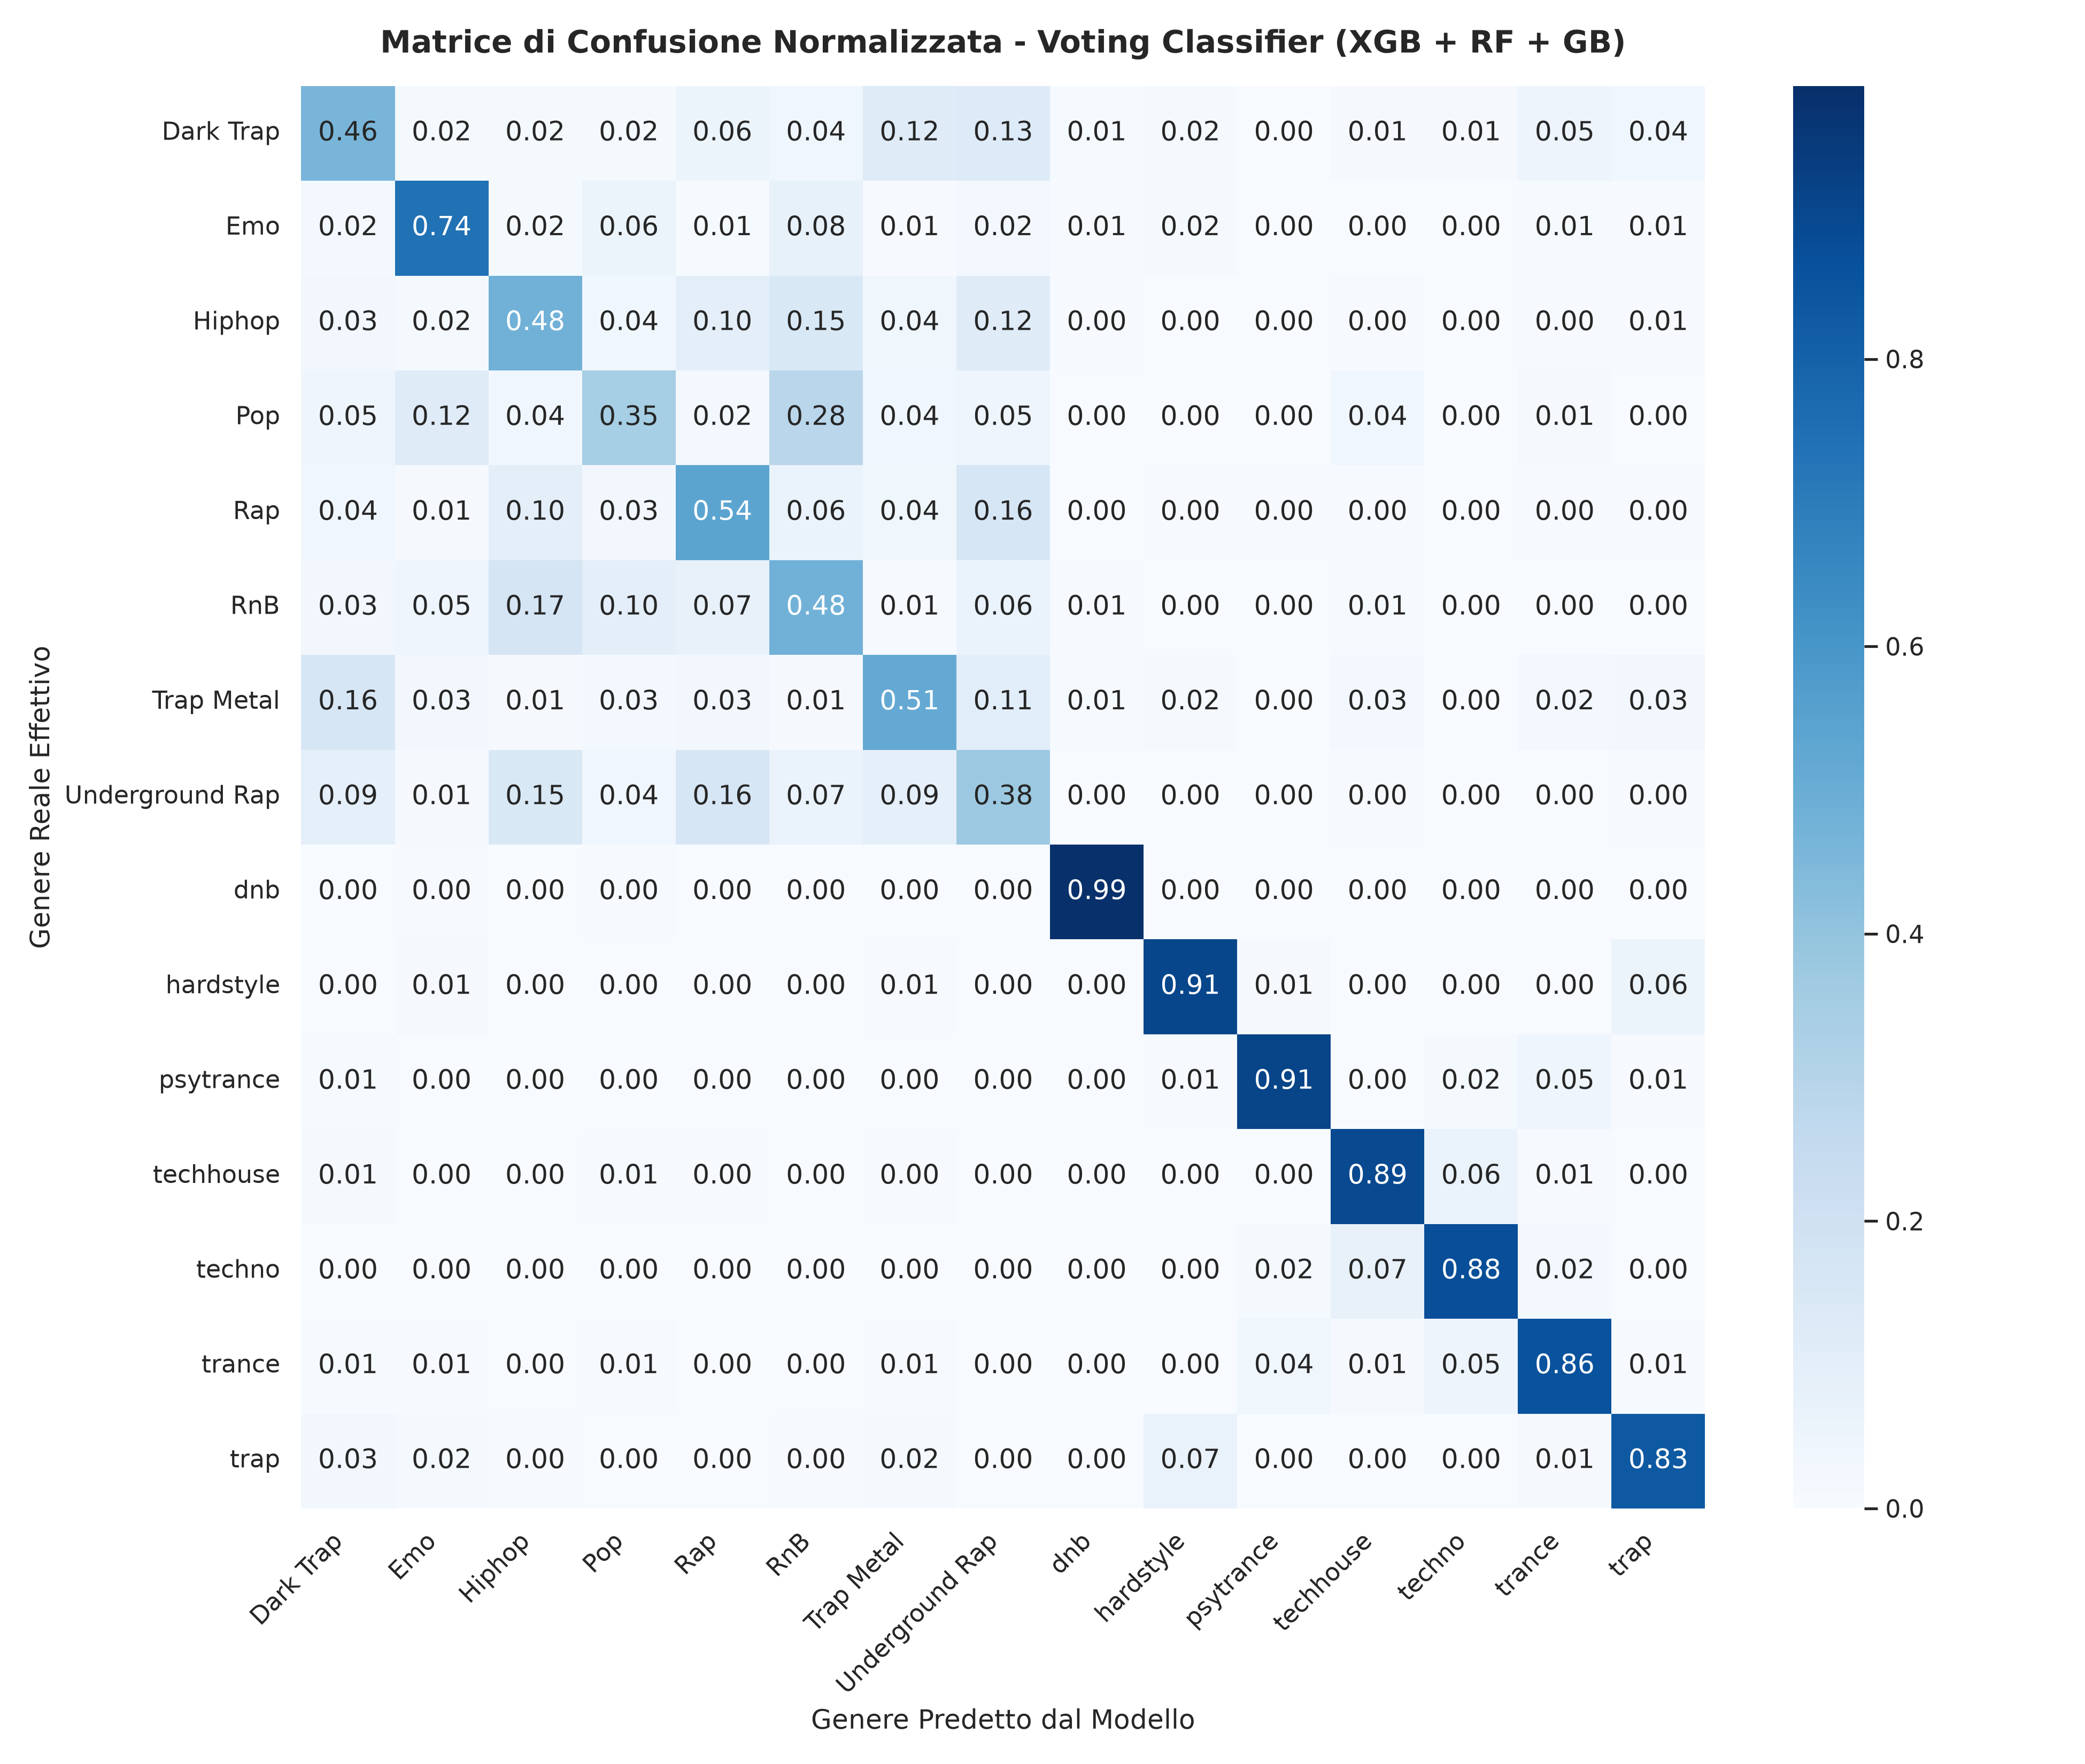
\includegraphics[width=0.88\textwidth]{figures/fig08_confusion_matrix_best_model.png}
    \caption{Matrice di confusione normalizzata per il modello Ensemble finale.}
    \label{fig:confusion_matrix}
\end{figure}

\begin{figure}[H]
    \centering
    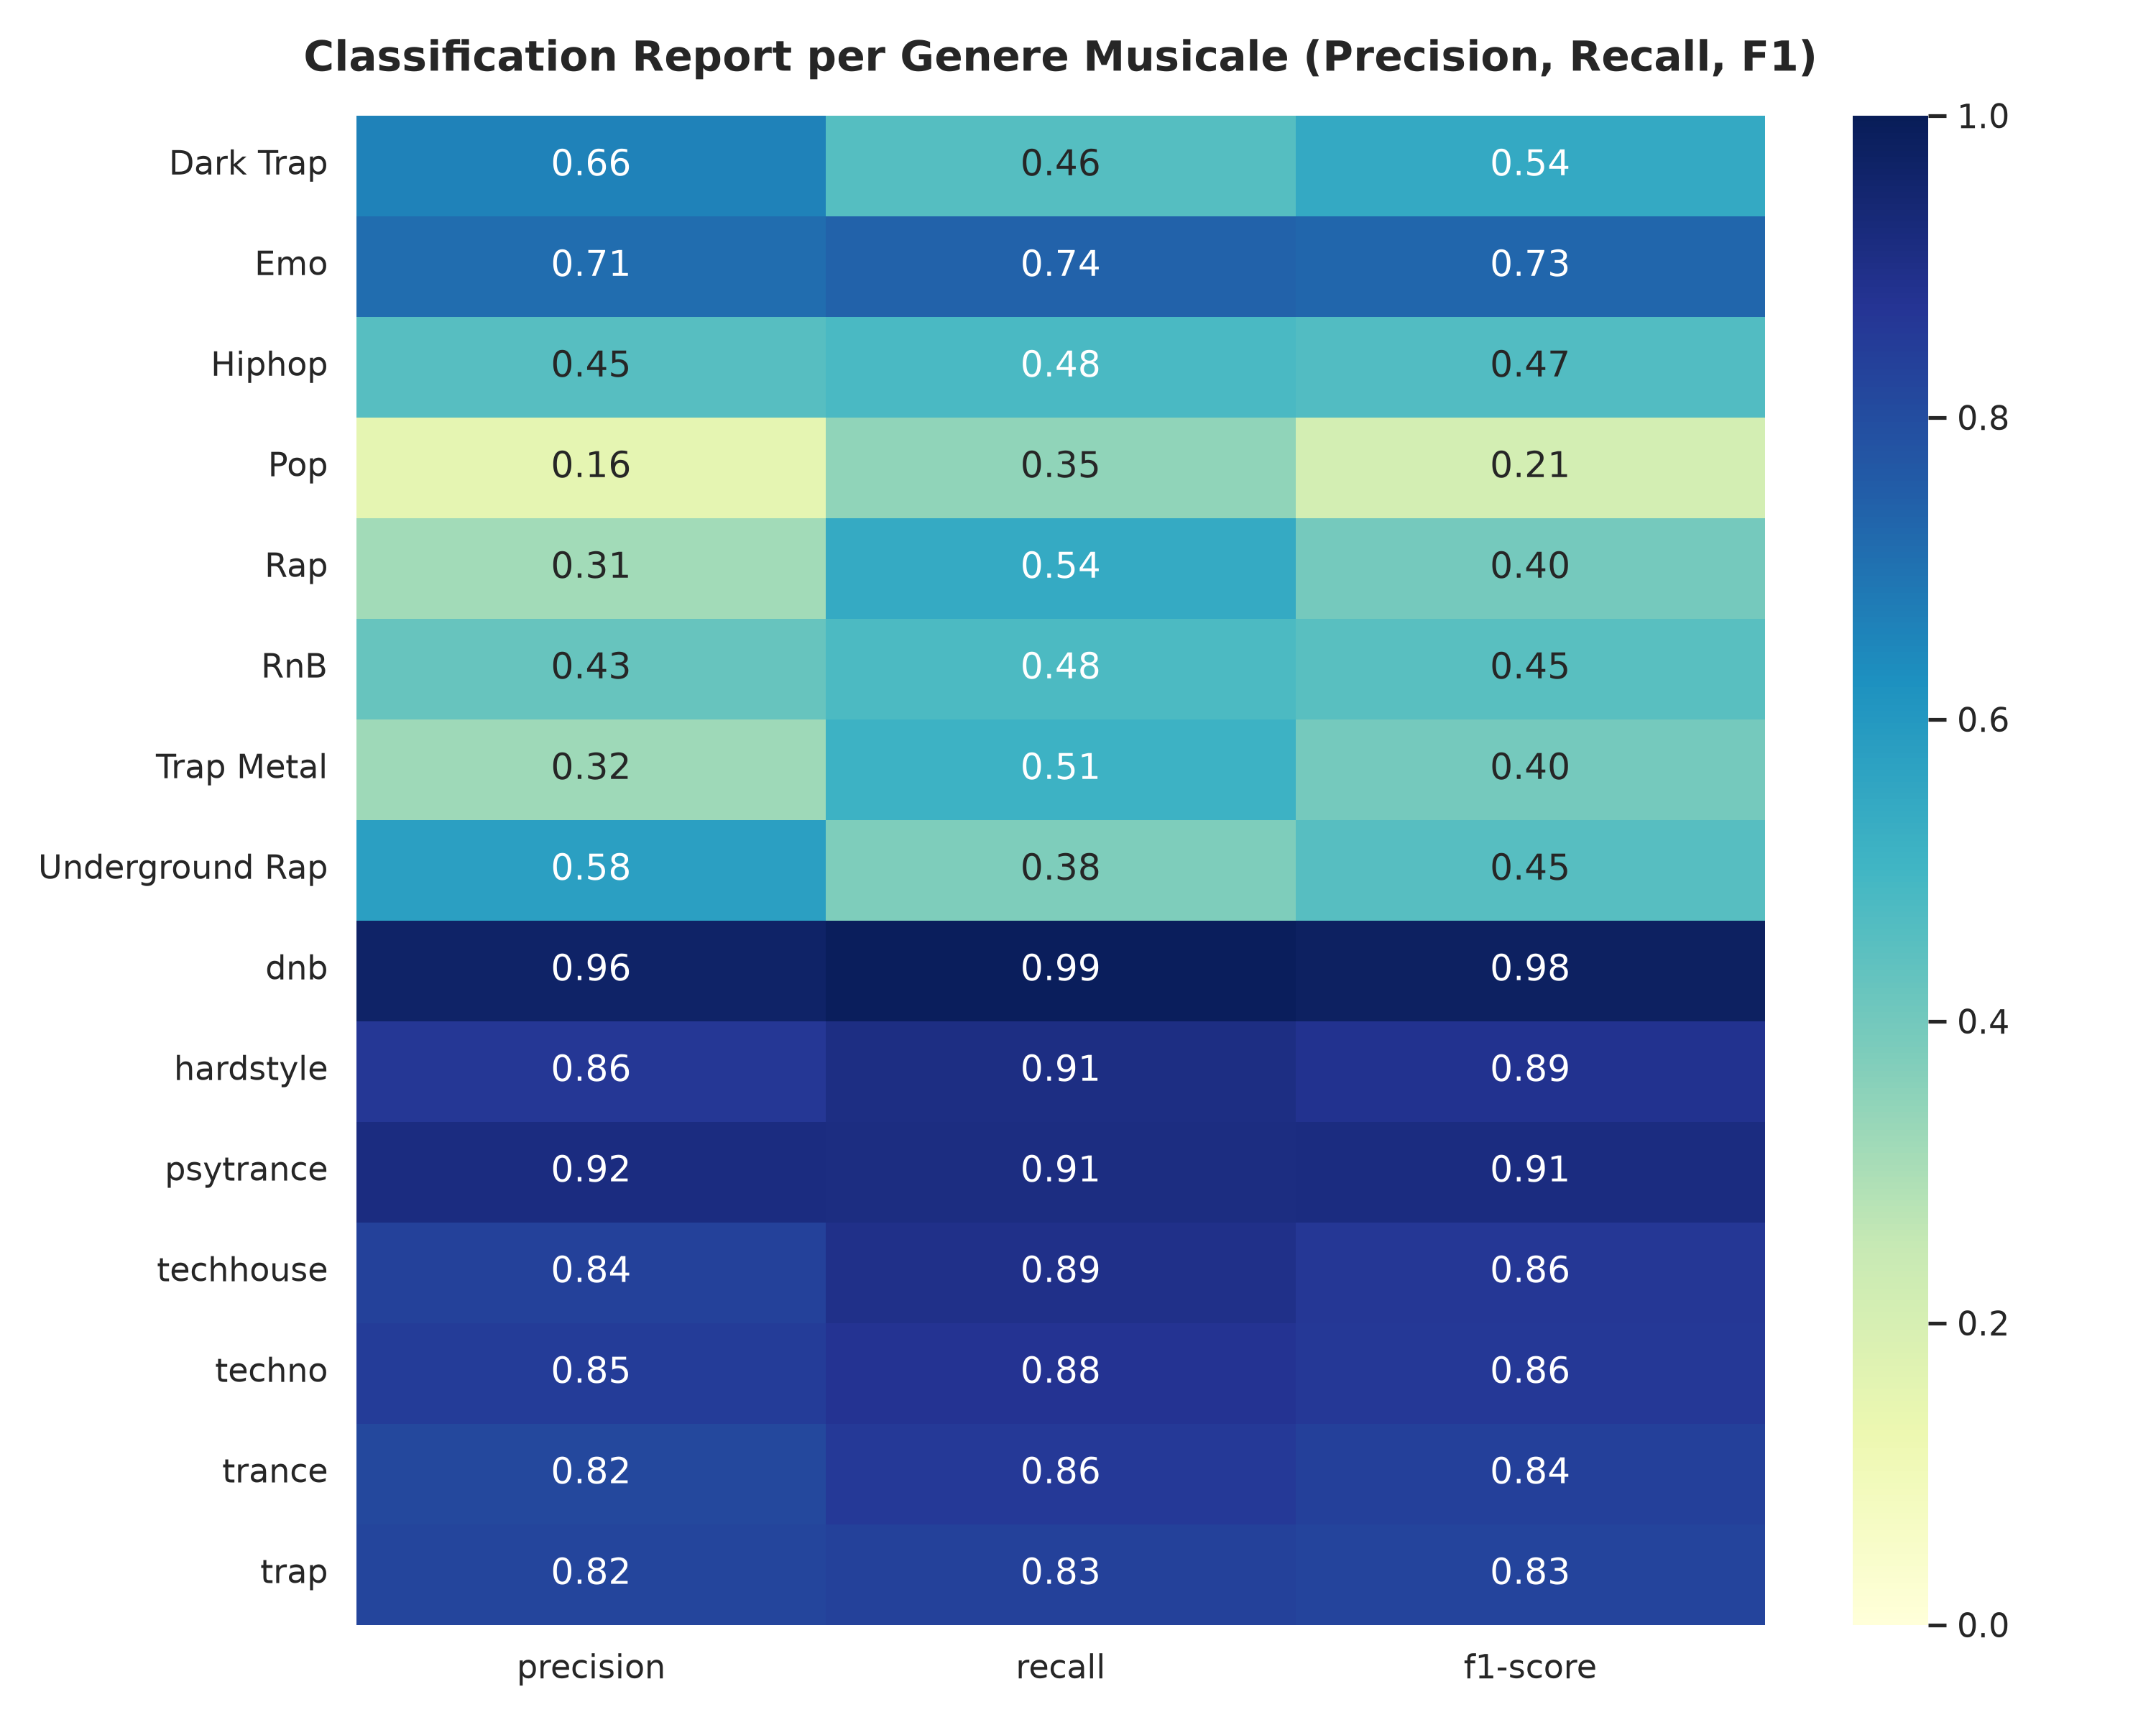
\includegraphics[width=0.75\textwidth]{figures/fig09_classification_report_heatmap.png}
    \caption{Classification Report per genere: valori di Precision, Recall ed F1-Score.}
    \label{fig:classification_report}
\end{figure}

\subsubsection{Curve ROC, Precision-Recall e Learning Curve}
In Figura \ref{fig:roc_pr_curves} vengono mostrate le curve ROC (One-vs-Rest) e le curve Precision-Recall. Il valore di \textbf{Macro-Average ROC-AUC è pari a 0.94}, con diverse classi che raggiungono valori di AUC superiori a \textbf{0.97}, a testimonianza di una forte capacità discriminante su scala globale.

La Learning Curve riportata in Figura \ref{fig:learning_curve} conferma che, con l'incremento dei campioni di training, la curva di validazione sale costantemente avvicinandosi a quella di addestramento con un gap contenuto, escludendo fenomeni di overfitting.

\begin{figure}[H]
    \centering
    \begin{subfigure}[b]{0.49\textwidth}
        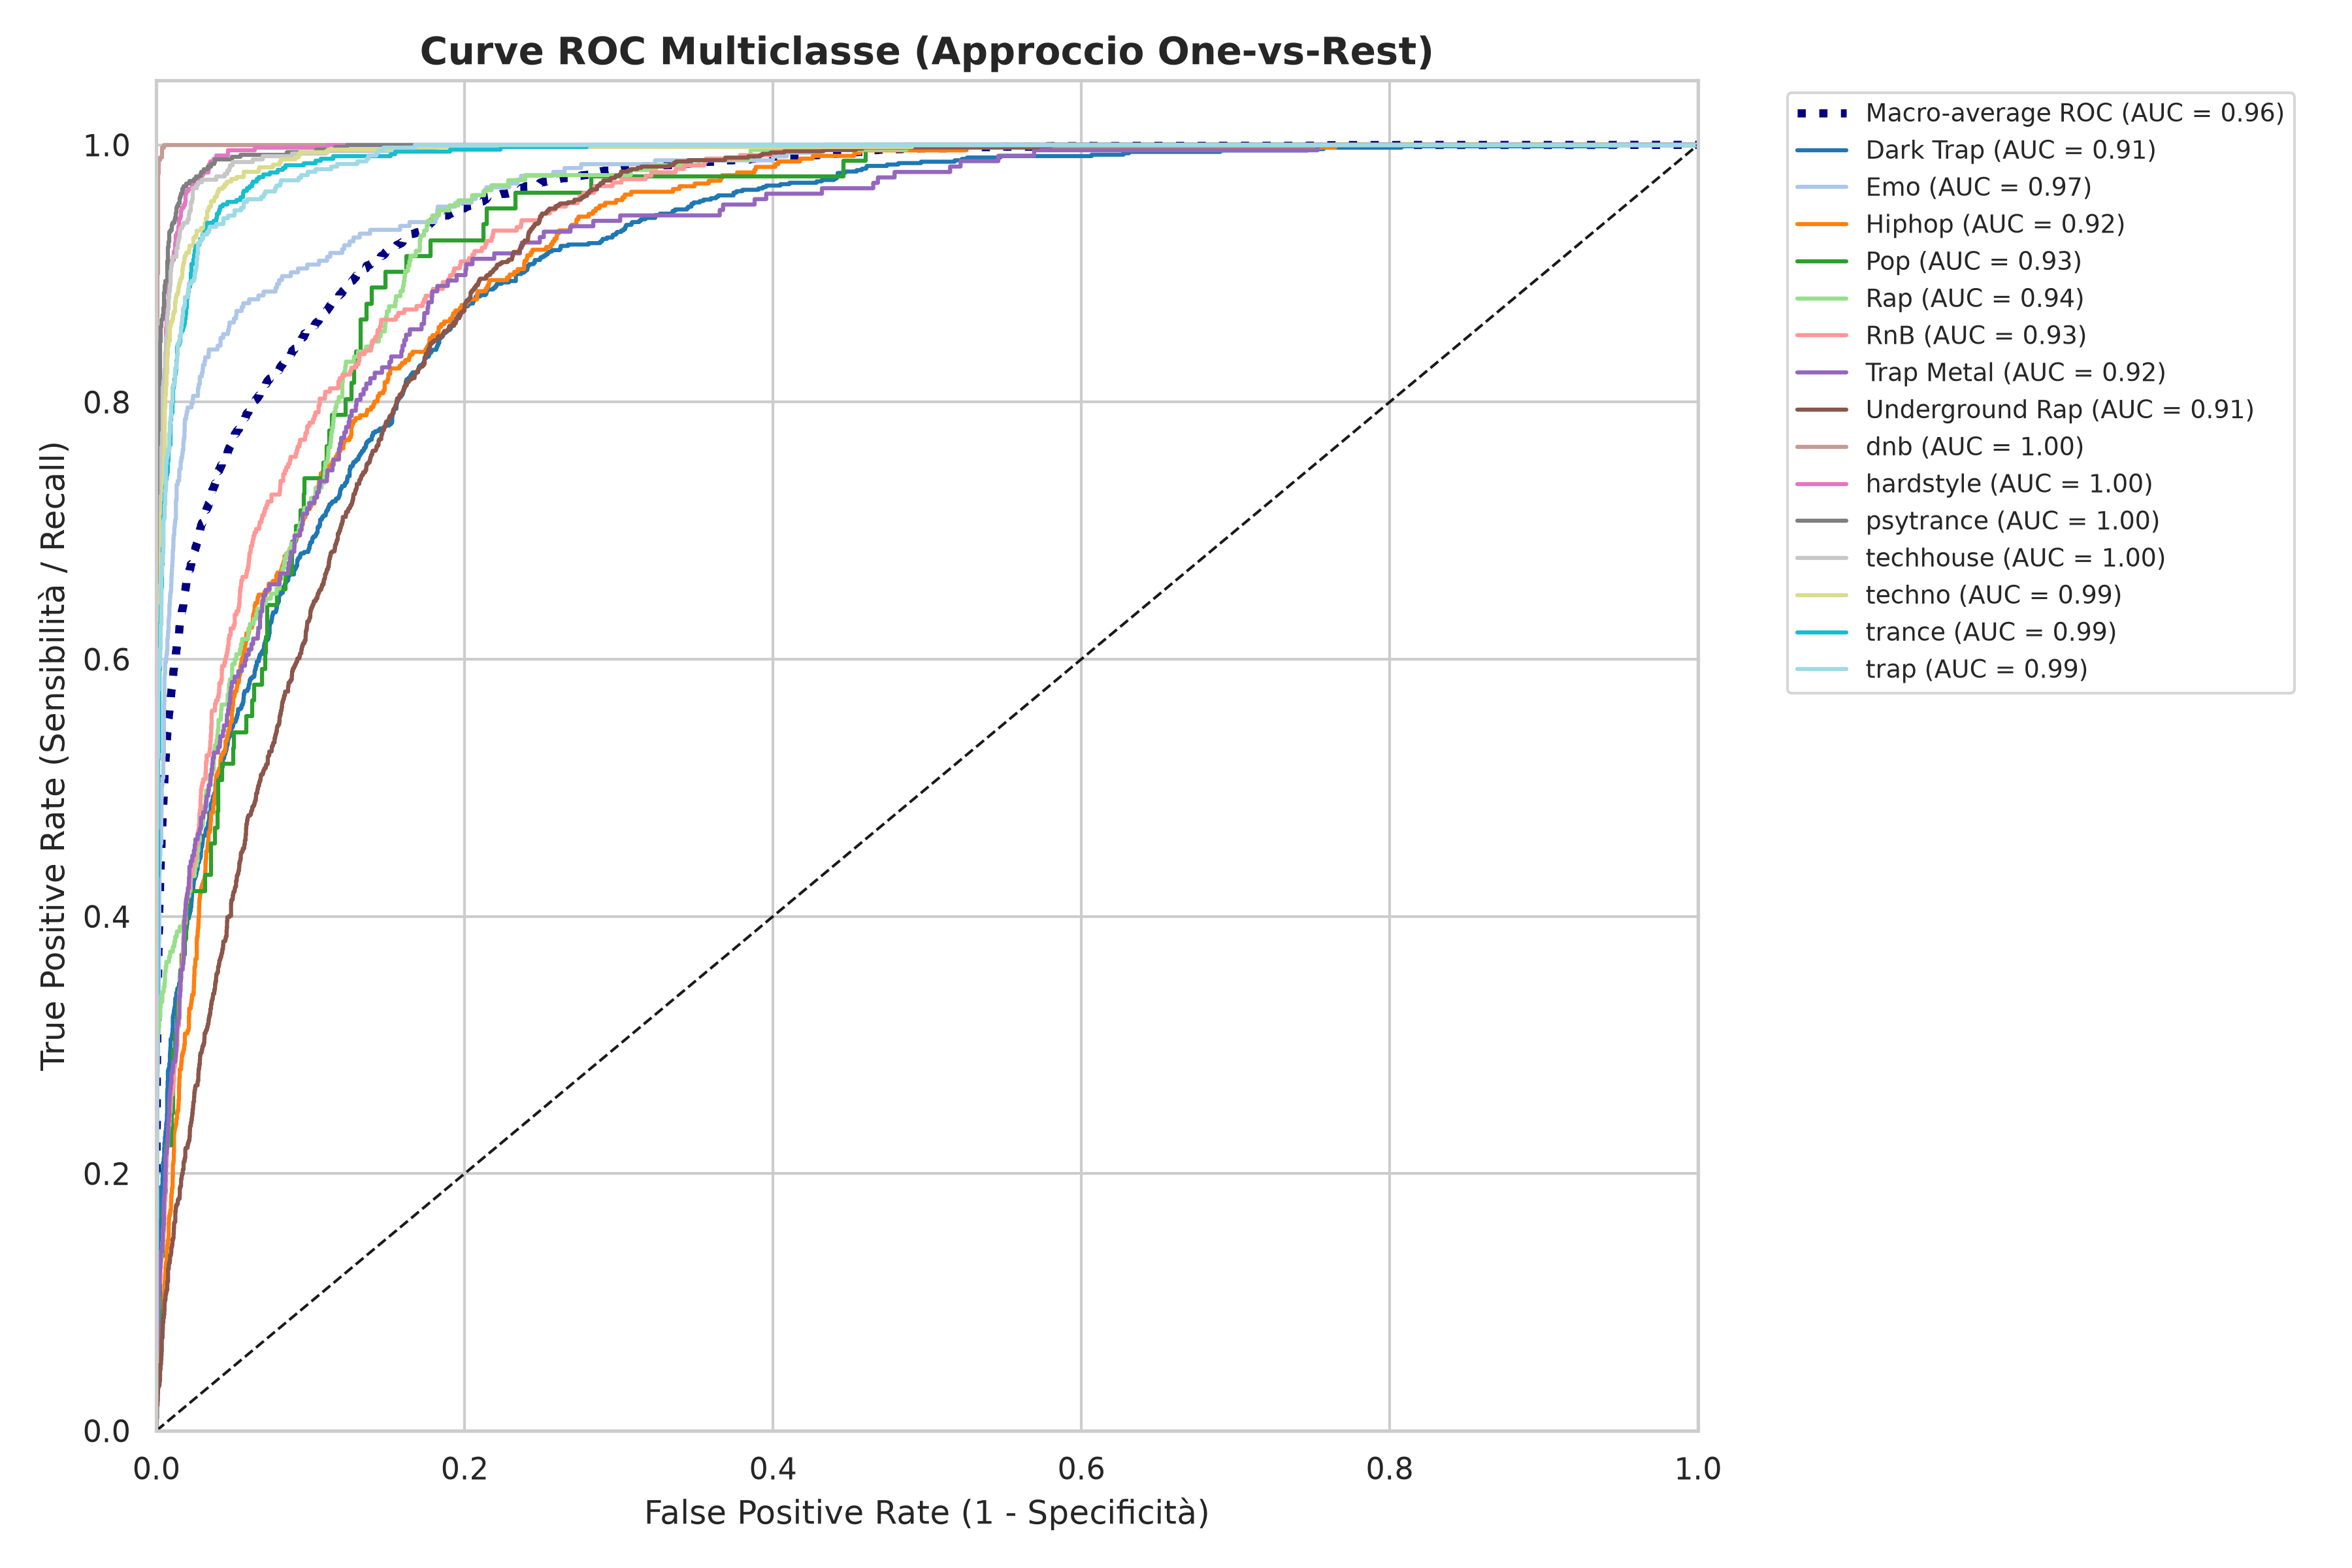
\includegraphics[width=\textwidth]{figures/fig10_roc_curves_multiclass.png}
        \caption{Curve ROC Multiclasse One-vs-Rest (Macro AUC = 0.94).}
    \end{subfigure}
    \hfill
    \begin{subfigure}[b]{0.49\textwidth}
        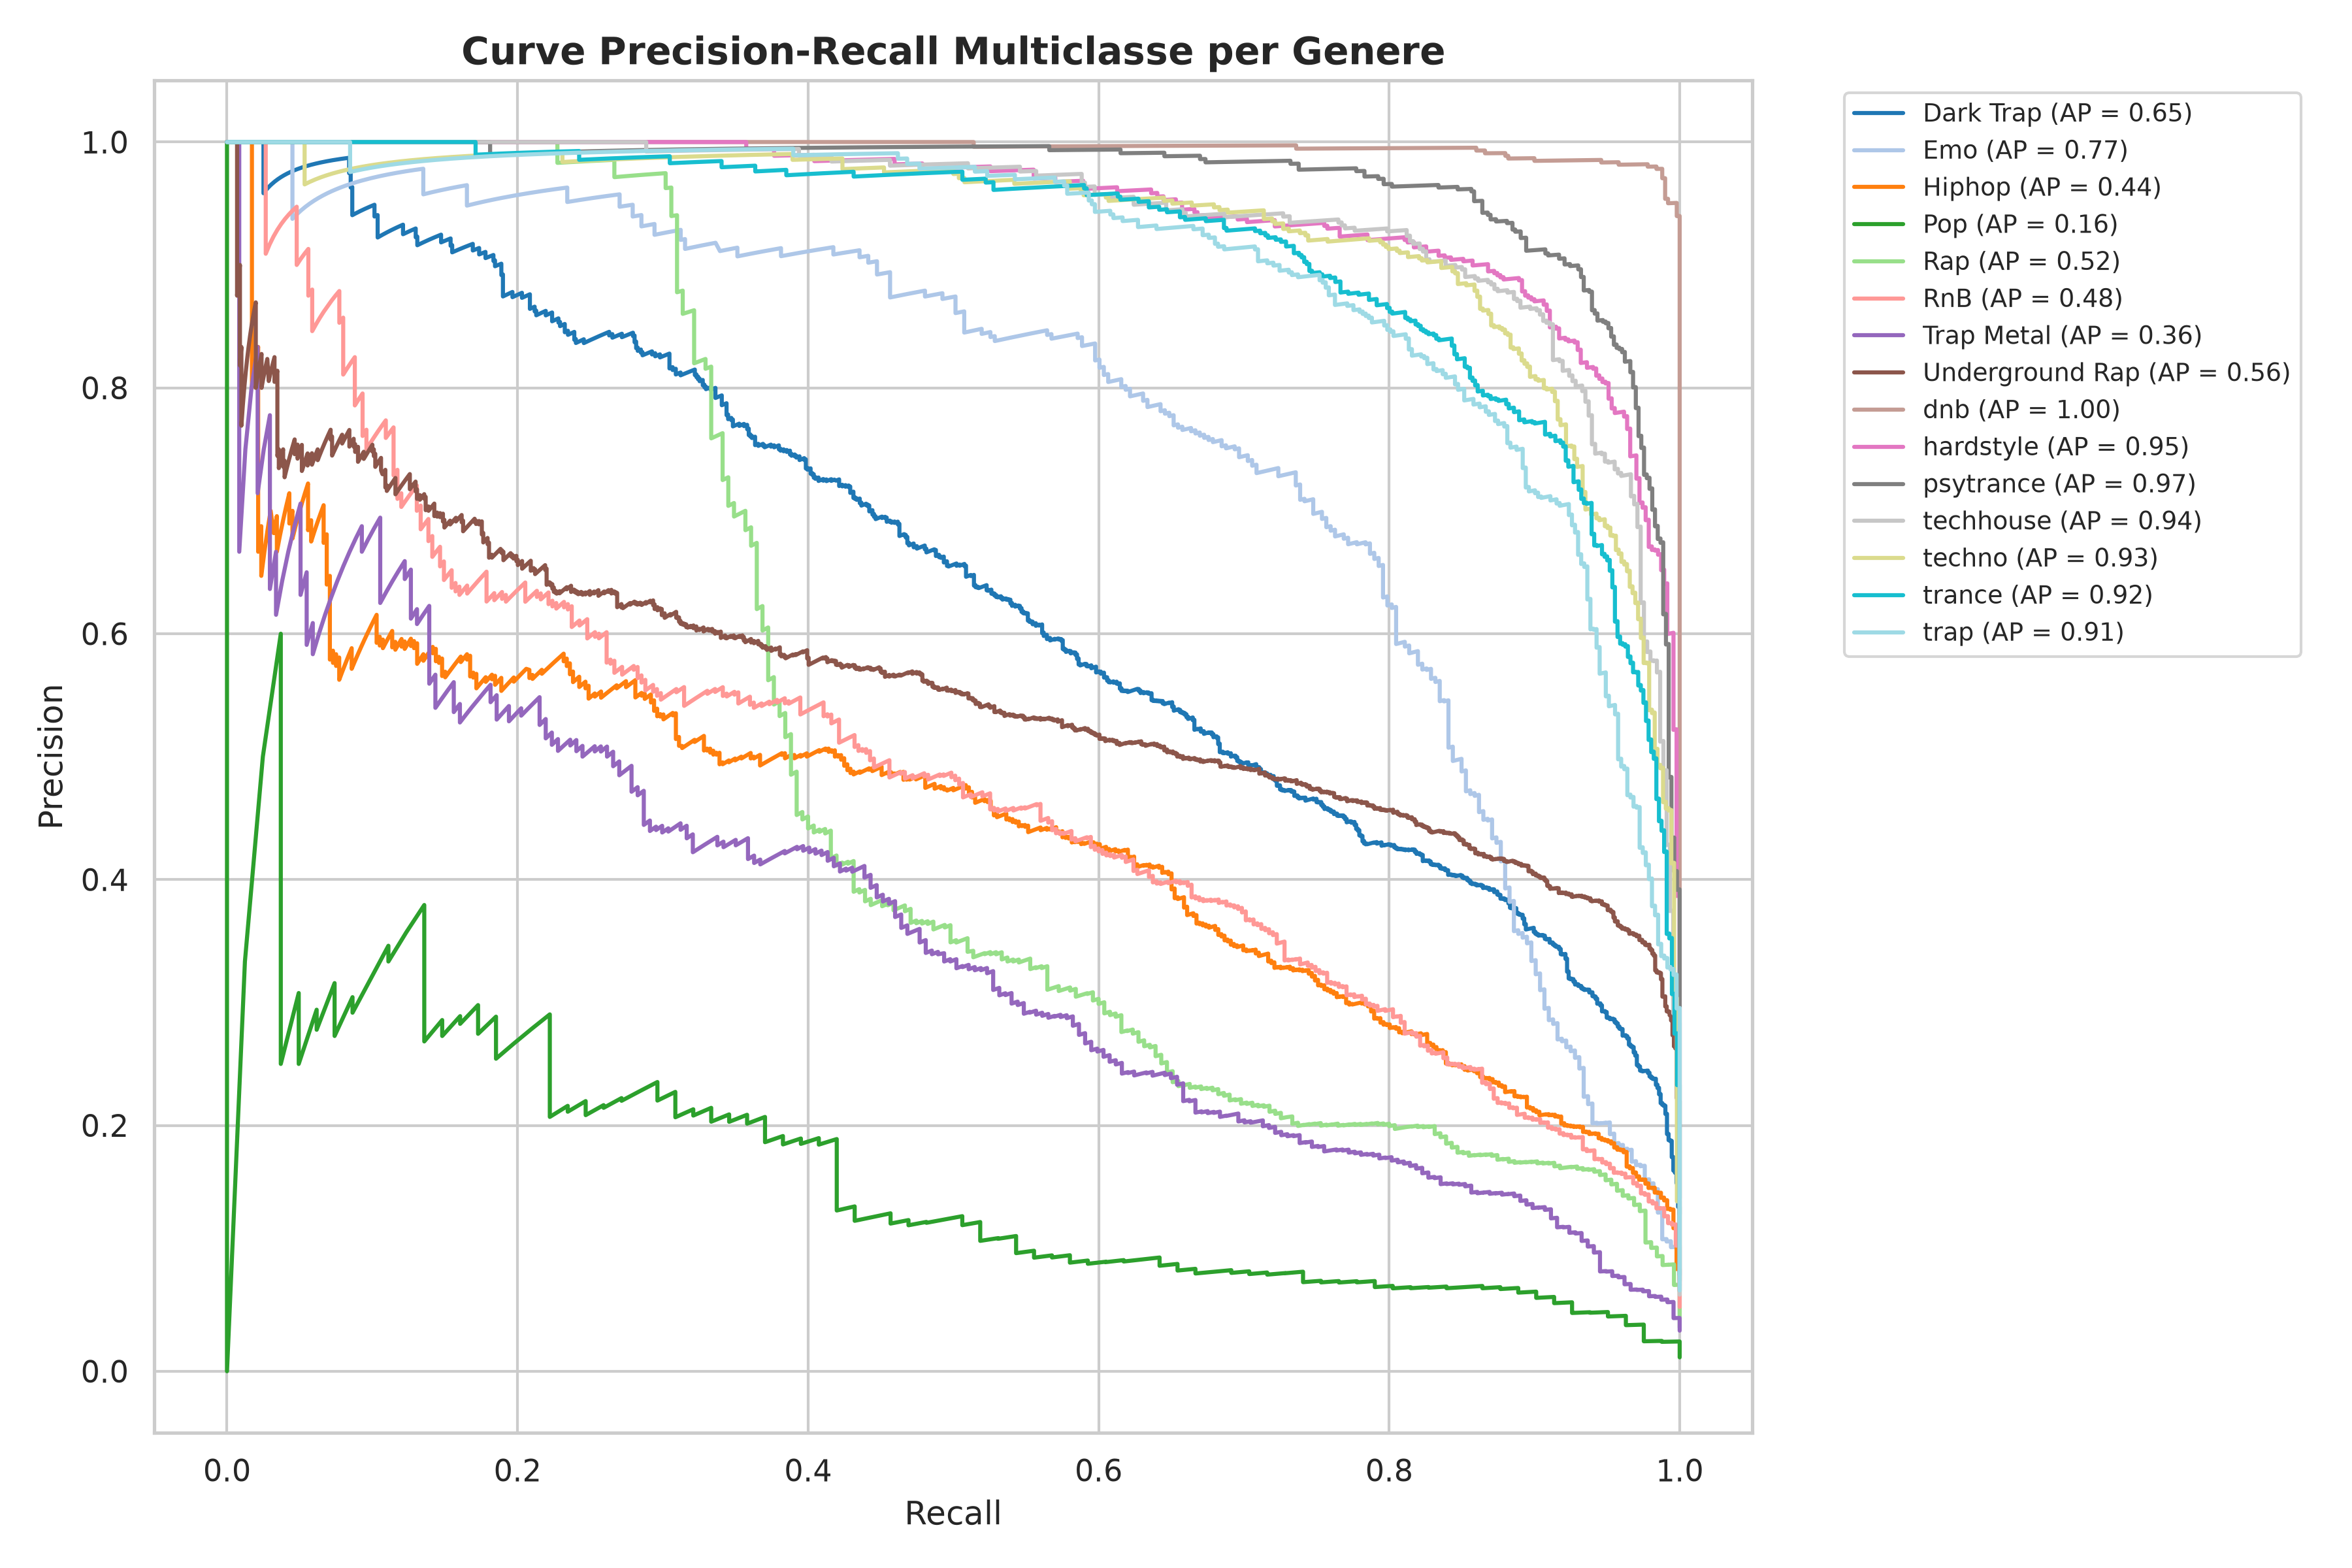
\includegraphics[width=\textwidth]{figures/fig11_precision_recall_curves.png}
        \caption{Curve Precision-Recall Multiclasse.}
    \end{subfigure}
    \caption{Valutazione delle curve ROC e Precision-Recall per tutte le classi di genere.}
    \label{fig:roc_pr_curves}
\end{figure}

\begin{figure}[H]
    \centering
    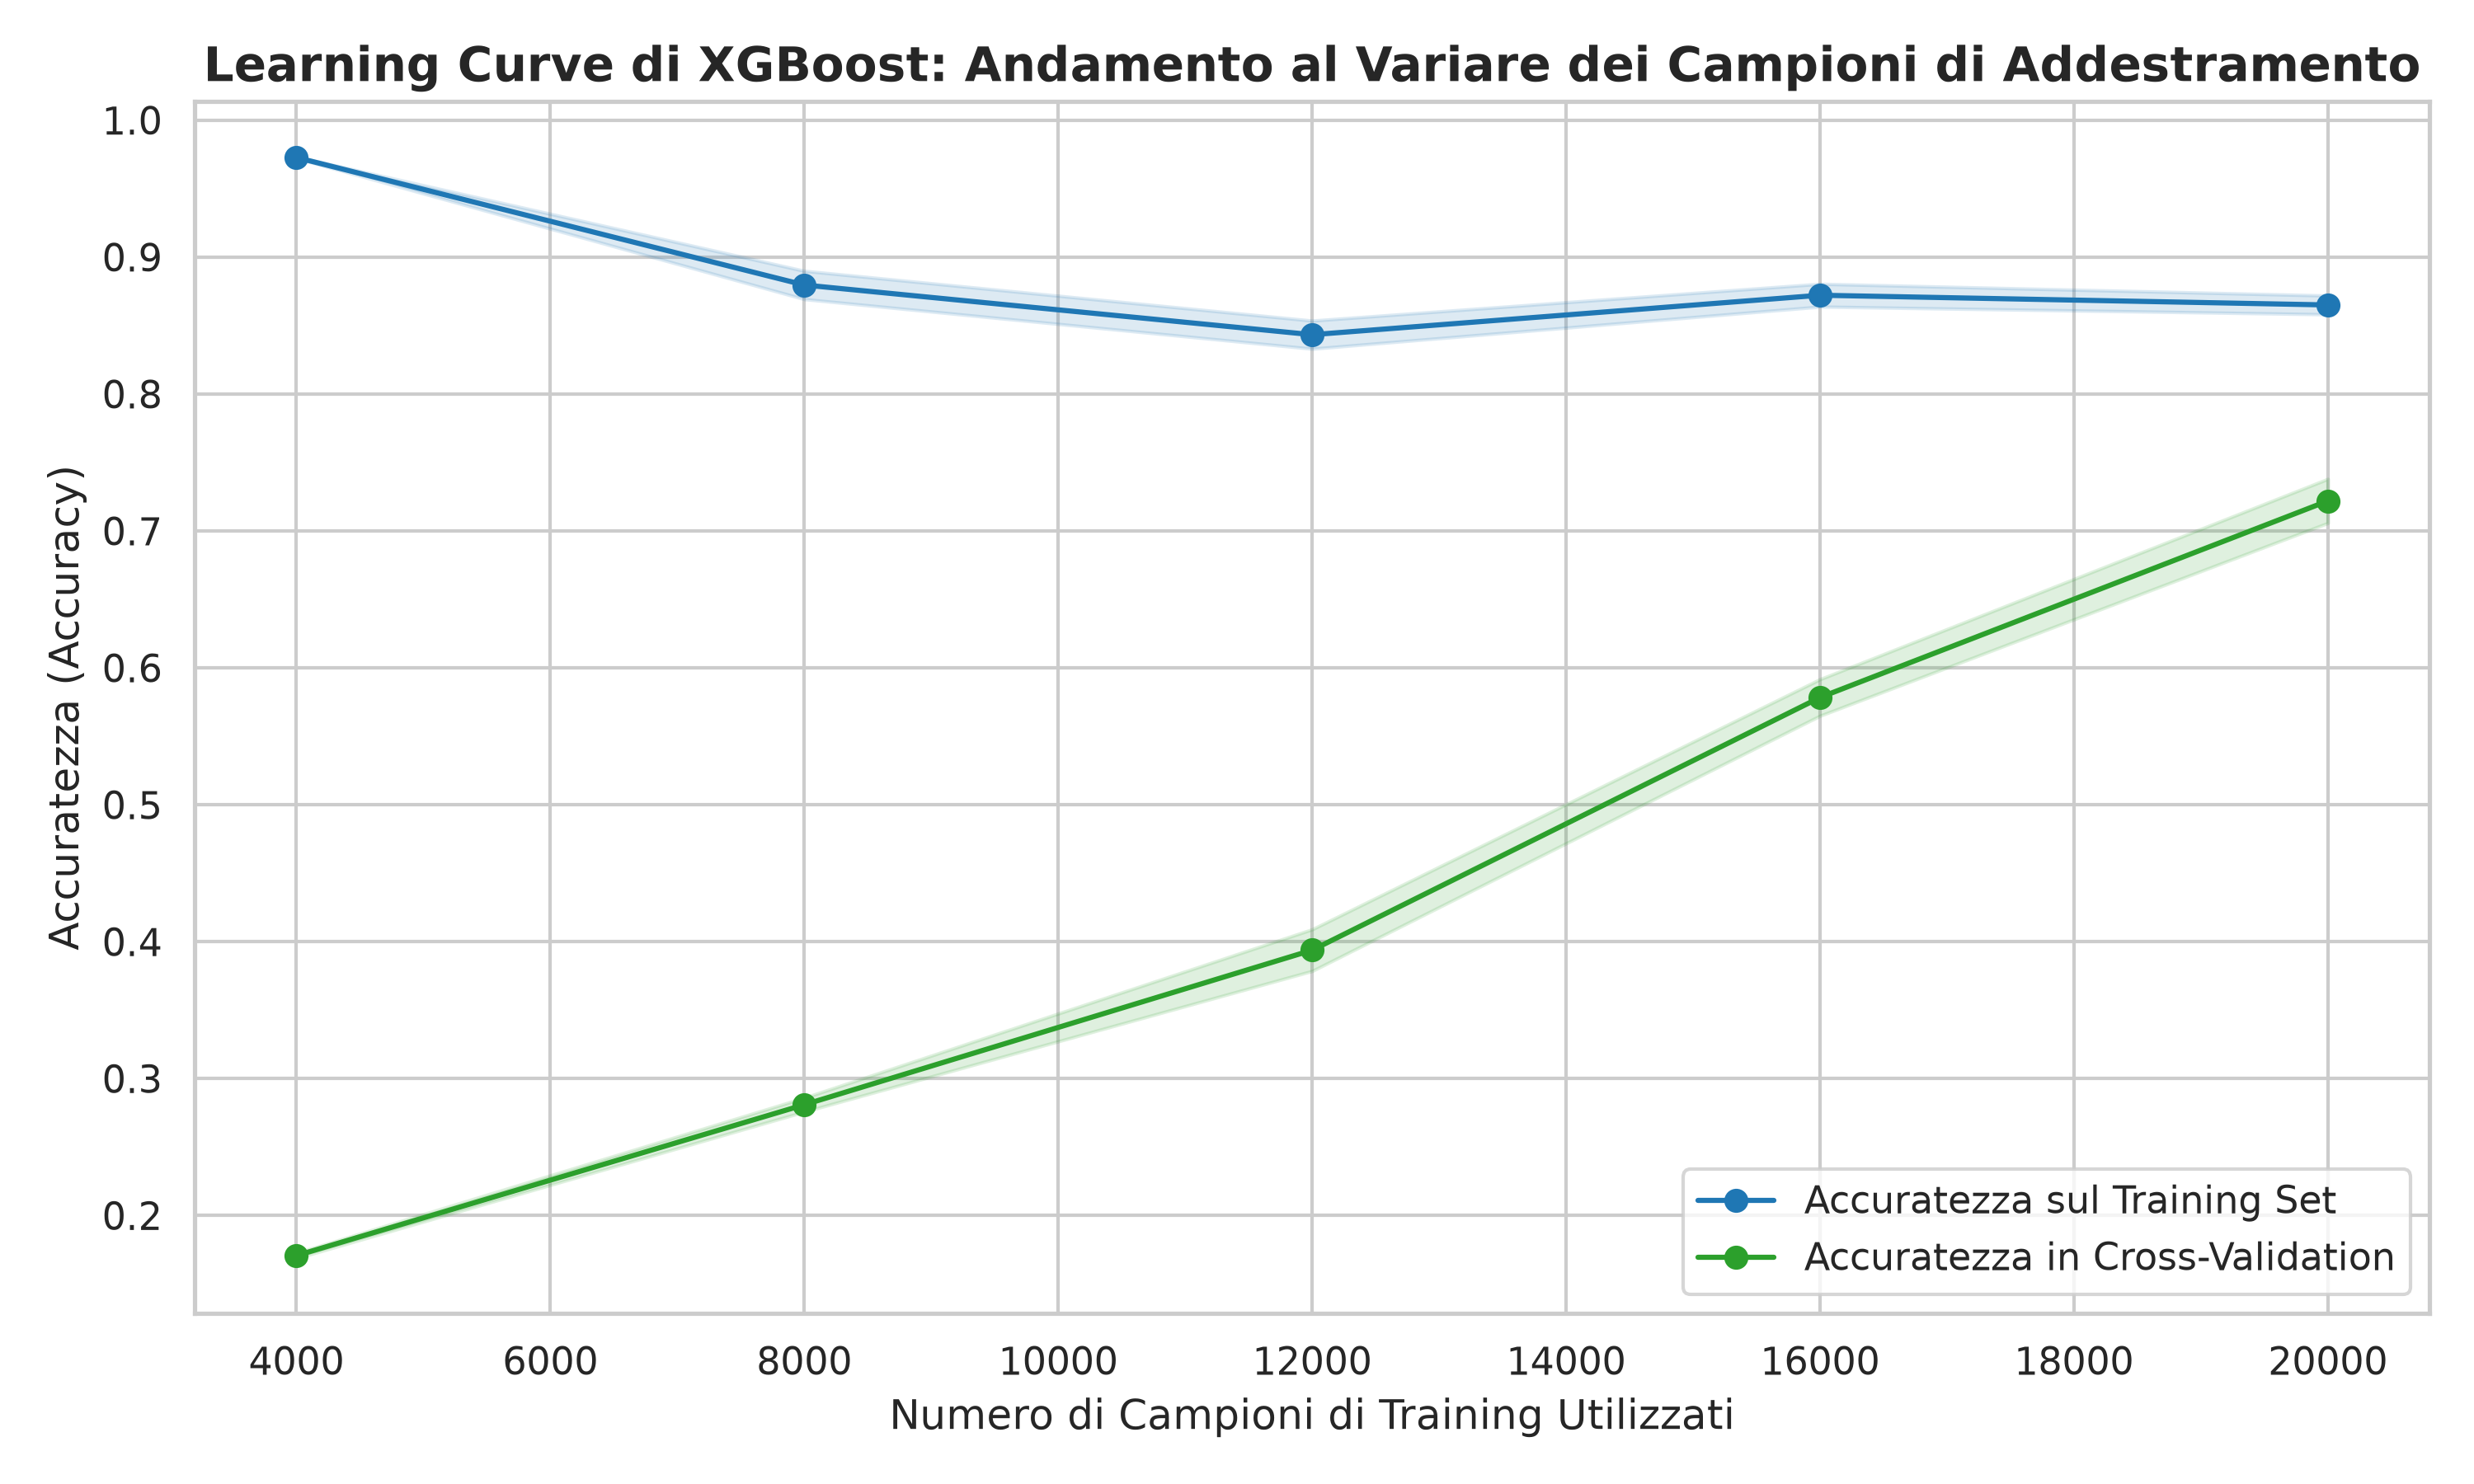
\includegraphics[width=0.80\textwidth]{figures/fig12_learning_curve.png}
    \caption{Learning Curve calcolata su XGBoost al variare dei campioni di training.}
    \label{fig:learning_curve}
\end{figure}

\subsubsection{Feature Importance}
La Figura \ref{fig:feature_importance} evidenzia l'importanza relativa delle feature estratta da Random Forest e XGBoost.
I fattori con il più elevato potere informativo risultano essere:
\begin{itemize}
    \item \texttt{tempo} (BPM): Separa immediatamente i generi elettronici veloci (\textit{DnB} a 174 BPM, \textit{Hardstyle} a 150 BPM) dai generi urban a tempo moderato.
    \item \texttt{speechiness}: Isola chiaramente i brani rap/trap ad alta densità di testo rispetto ai generi strumentali.
    \item \texttt{danceability}, \texttt{loudness} ed \texttt{energy}: Determinano il mood e la compattezza dinamica.
\end{itemize}

\begin{figure}[H]
    \centering
    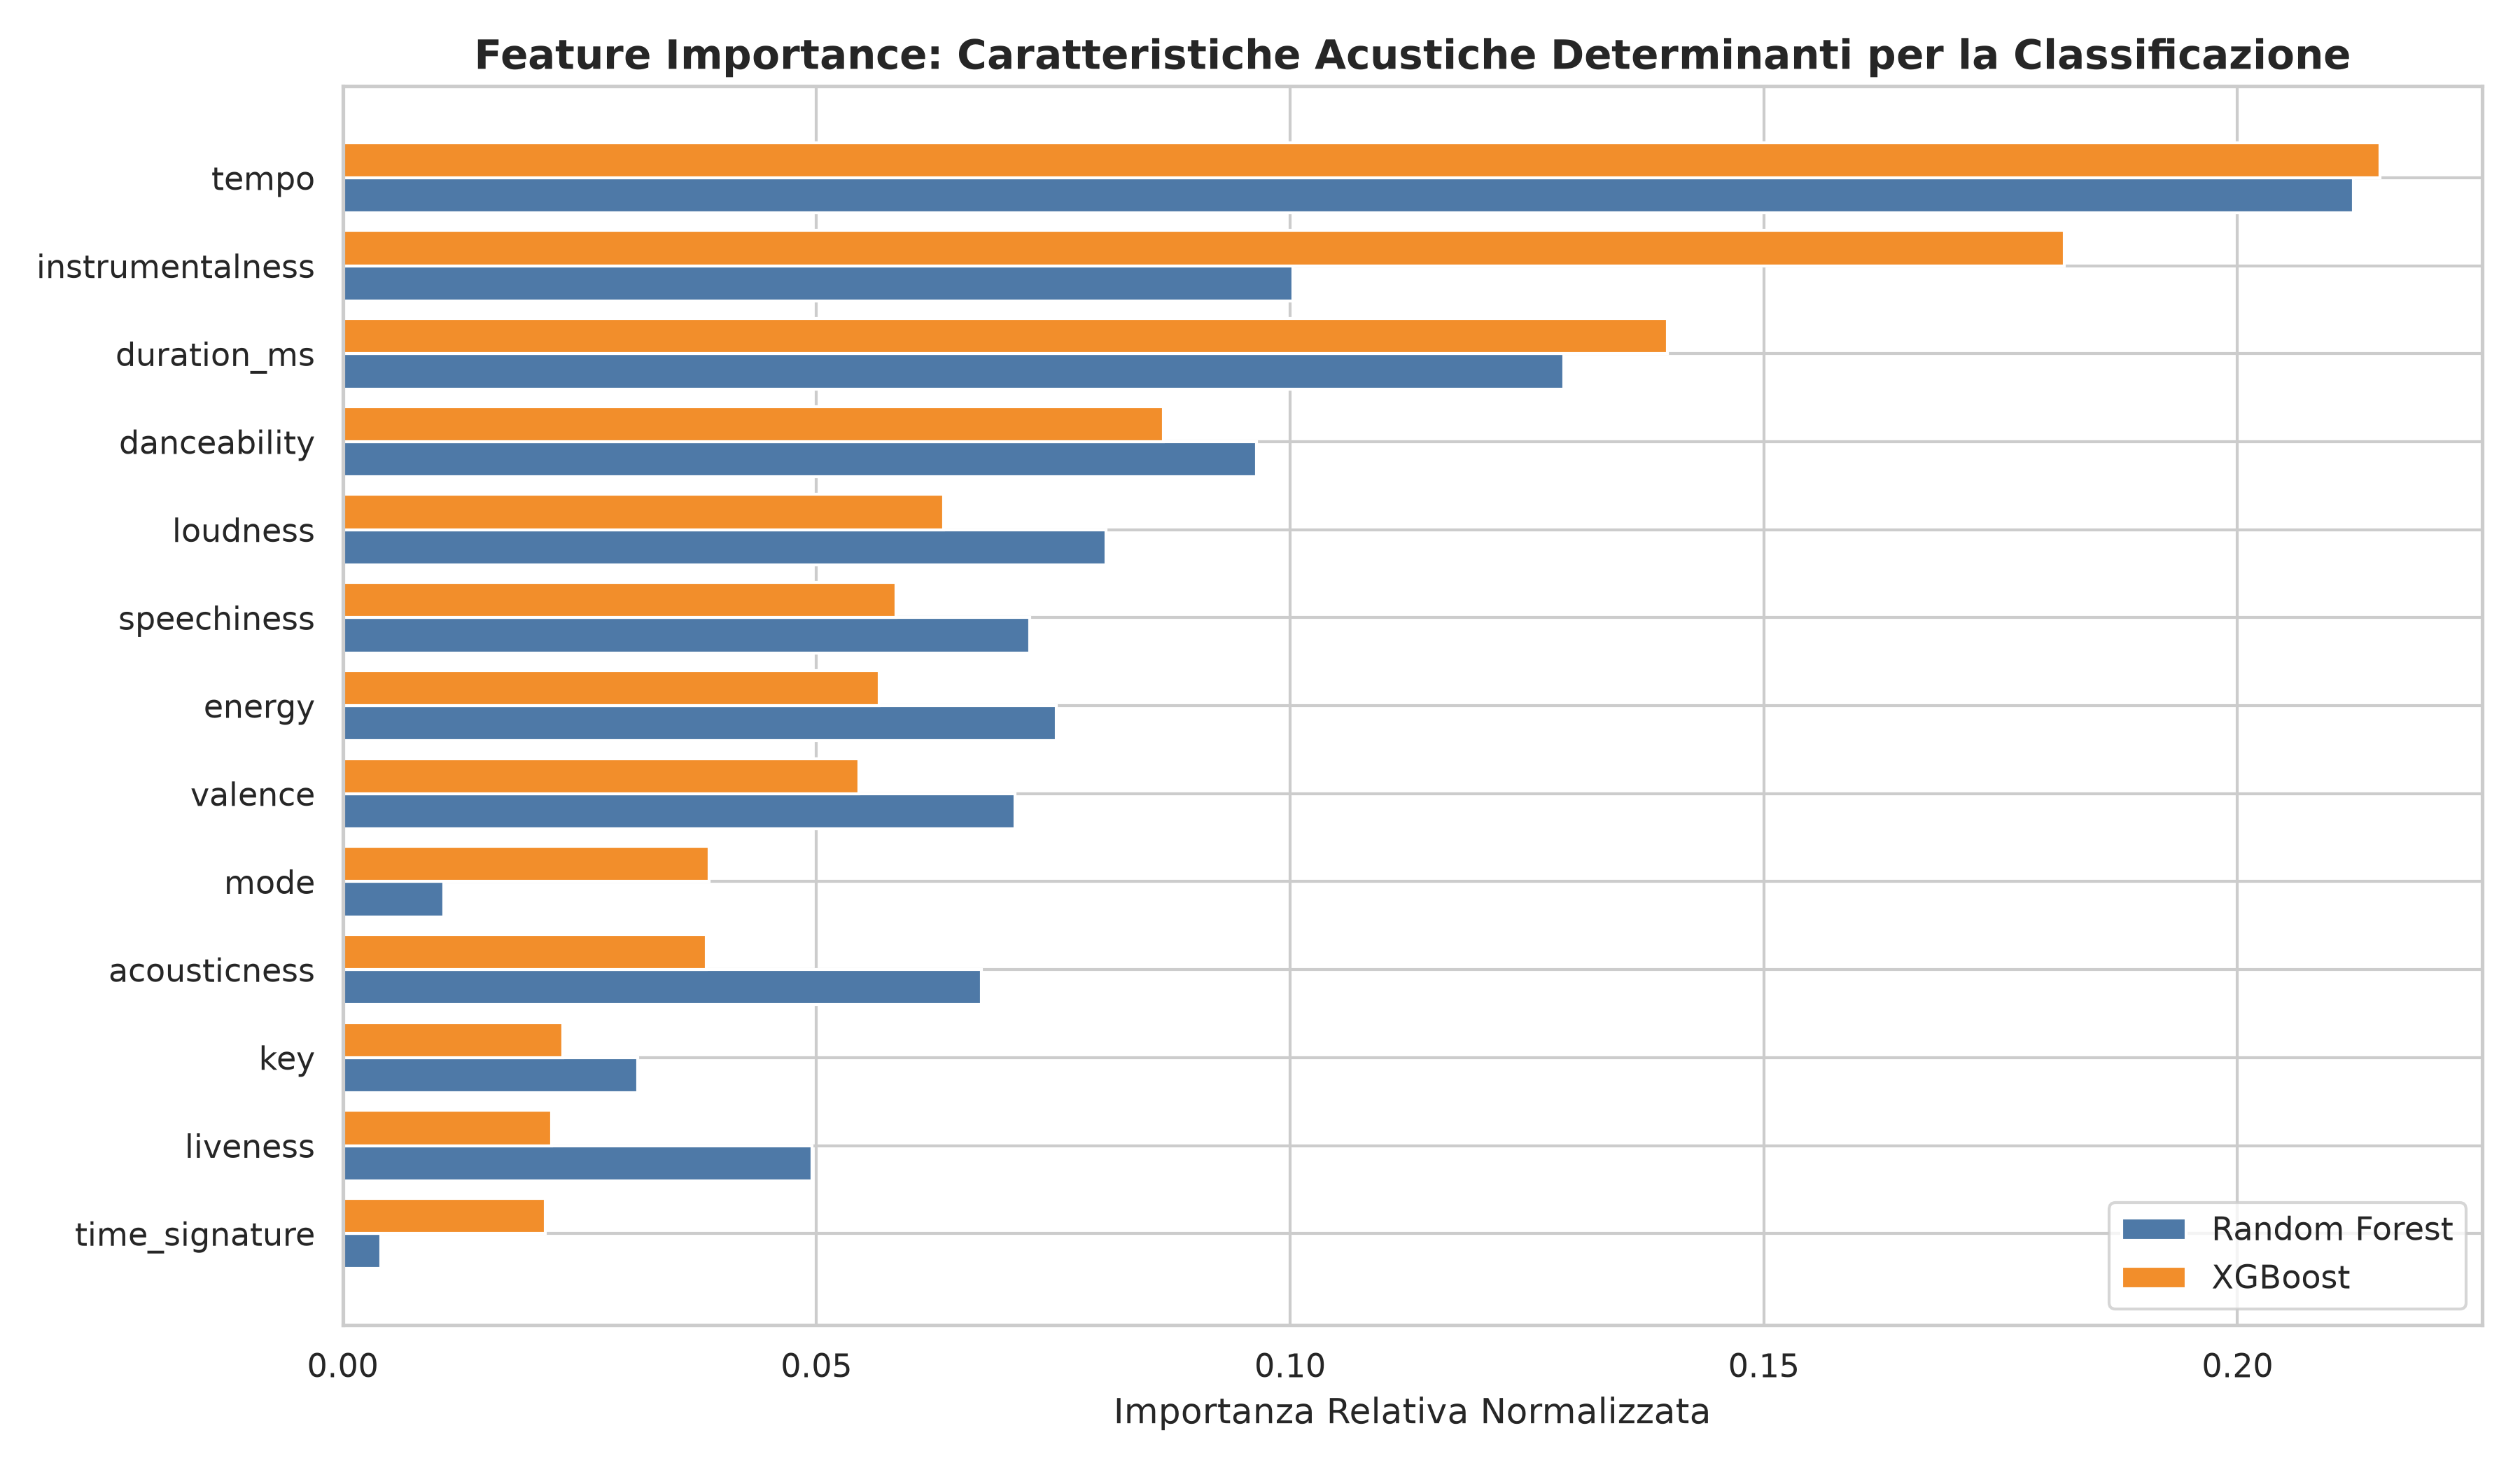
\includegraphics[width=0.85\textwidth]{figures/fig13_feature_importance.png}
    \caption{Feature Importance: confronto tra Random Forest e XGBoost.}
    \label{fig:feature_importance}
\end{figure}

\newpage
% =========================================================================
% CAPITOLO 4: CLUSTERING
% =========================================================================
\section{Spotify tracks analysis: Clustering}

Questo capitolo illustra l'applicazione di tecniche di clusterizzazione con lo scopo di raggruppare i brani musicali sulla base esclusiva delle loro proprietà acustiche intrinseche, in modo completamente non supervisionato ed escludendo la colonna \texttt{genre}. Gli algoritmi considerati ricadono nelle categorie di \textbf{partizionamento} (K-Means) e \textbf{densità} (DBSCAN).

\subsection{Fase di ETL per il clustering}
\subsubsection{Operazioni preliminari sul dataset}
Gli attributi identificativi (\texttt{id}) e il target commerciale (\texttt{genre}) sono stati eliminati per rendere il modello agnostico rispetto alla categorizzazione di mercato ed evitare problemi legati alla \textit{curse of dimensionality}\footnote{La curse of dimensionality si verifica quando l'aumento delle feature disperde i dati nello spazio multidimensionale, riducendo l'efficacia del calcolo delle distanze.}. Tutte le feature audio numeriche sono state standardizzate mediante \texttt{StandardScaler}.

\subsubsection{Riduzione di dimensionalità (PCA e t-SNE)}
Al fine di analizzare e visualizzare la struttura dei cluster, sono state impiegate due tecniche complementari di riduzione di dimensionalità:
\begin{itemize}
    \item \textbf{Principal Component Analysis (PCA):} Dallo Scree Plot in Figura \ref{fig:pca_scree} emerge che le prime 6 componenti principali spiegano oltre il \textbf{70\% della varianza cumulativa totale}, evidenziando che gran parte della variabilità acustica è concentrata in un sottospazio ridotto.
    \item \textbf{t-SNE (t-Distributed Stochastic Neighbor Embedding):} Applicato con dimensione di output pari a 2, \texttt{perplexity} = 40 e \texttt{random\_state} = 42. In Figura \ref{fig:tsne_overview} viene mostrata la disposizione bidimensionale dei brani, evidenziando raggruppamenti geometrici naturali.
\end{itemize}

\begin{figure}[H]
    \centering
    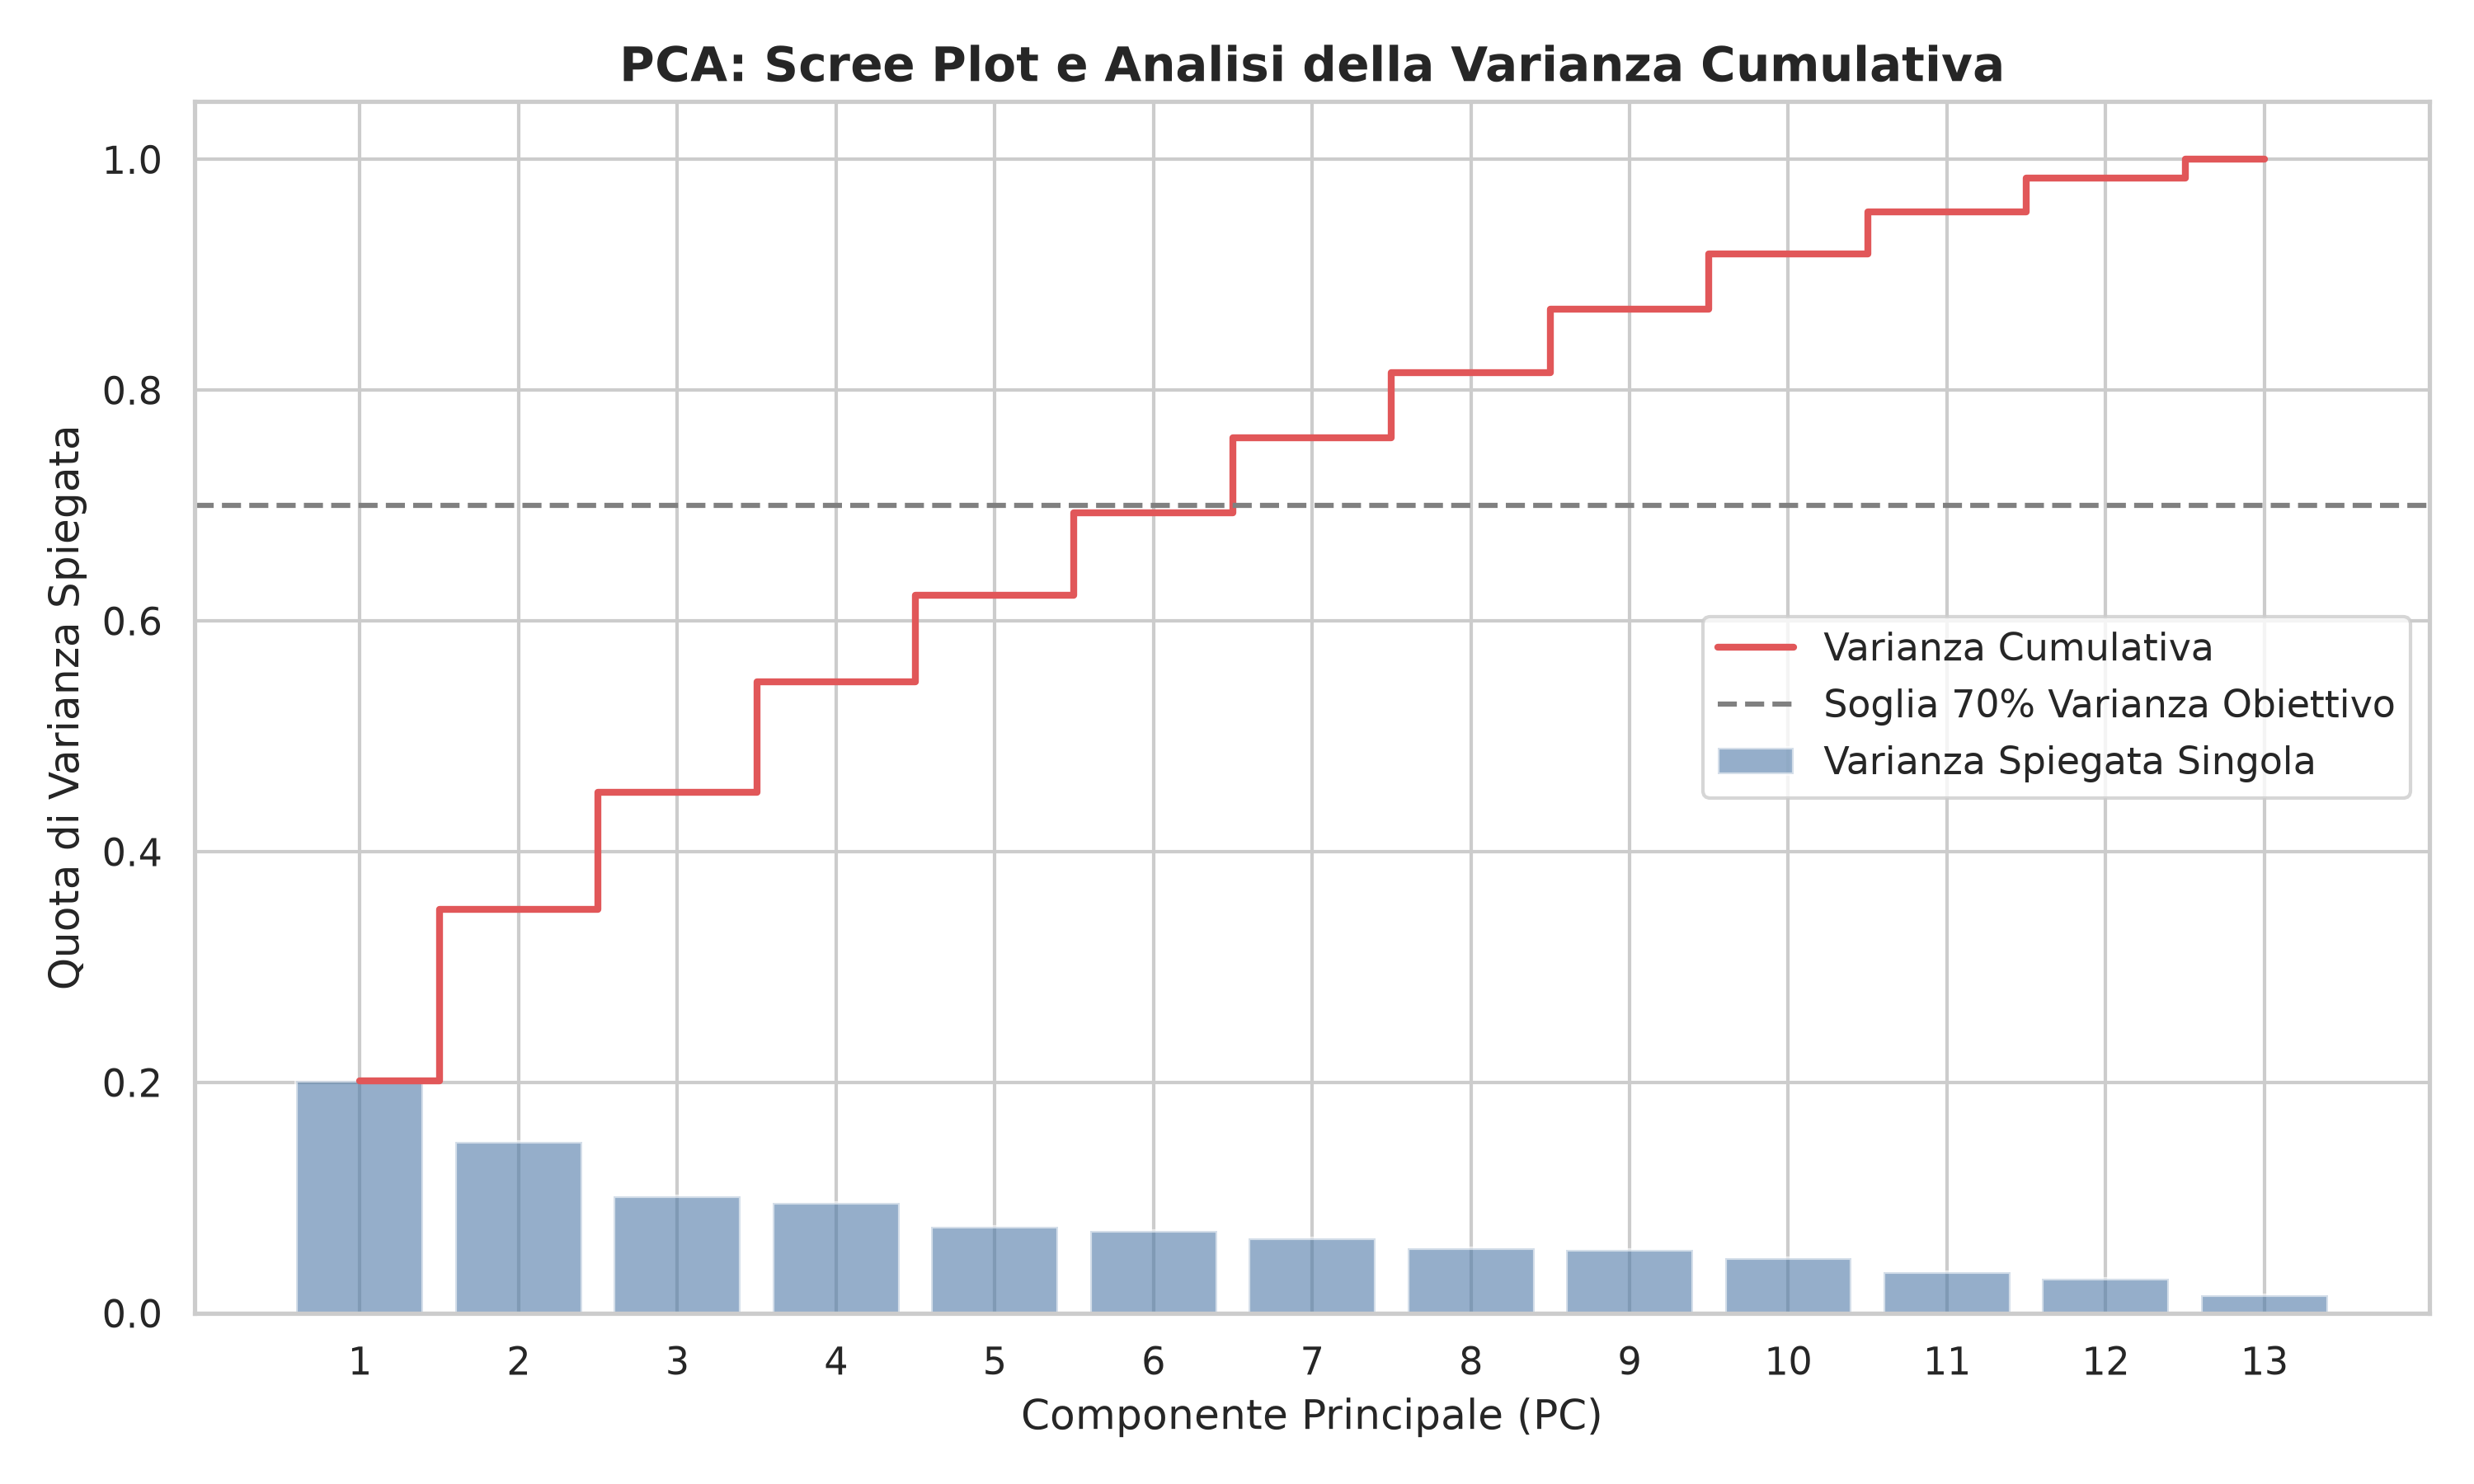
\includegraphics[width=0.75\textwidth]{figures/fig14_pca_varianza_cumulativa.png}
    \caption{PCA: Scree Plot della varianza spiegata individuale e cumulativa.}
    \label{fig:pca_scree}
\end{figure}

\begin{figure}[H]
    \centering
    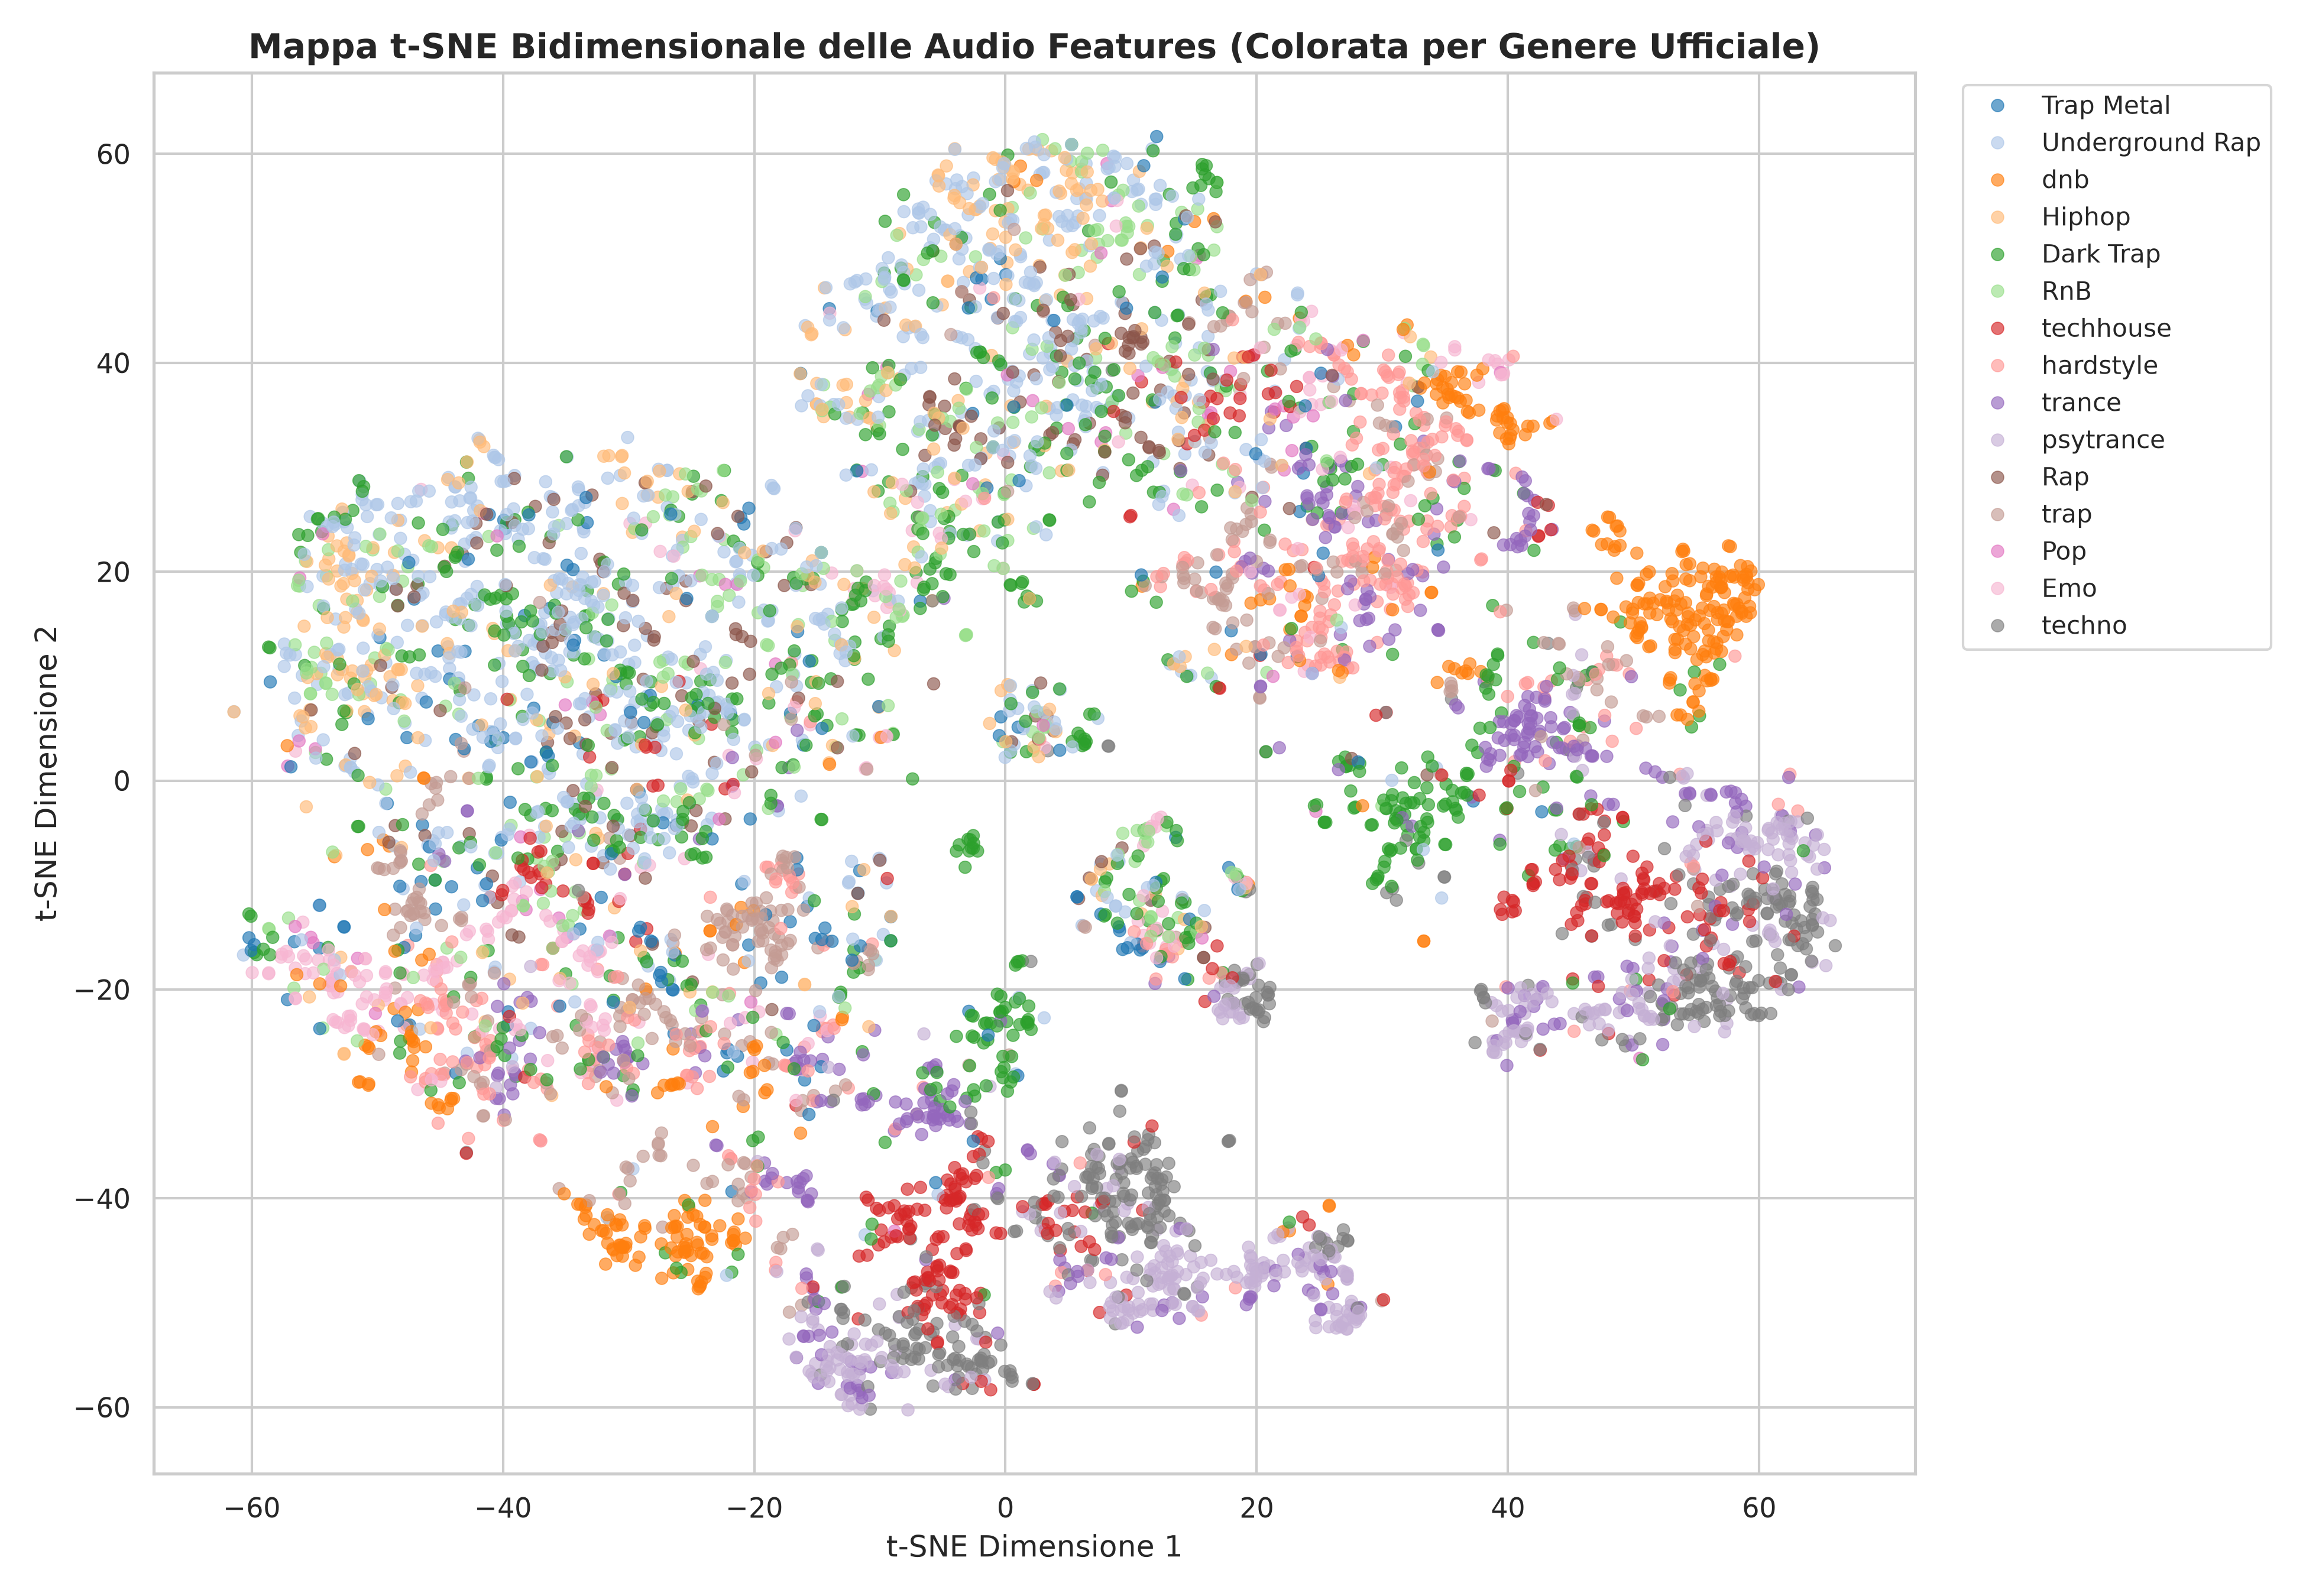
\includegraphics[width=0.88\textwidth]{figures/fig15_tsne_2d_overview.png}
    \caption{Mappa t-SNE 2D delle audio features con colorazione per genere Spotify originale.}
    \label{fig:tsne_overview}
\end{figure}

\subsection{Kmeans}
L'algoritmo K-Means suddivide le osservazioni in $k$ cluster cercando di minimizzare la somma dei quadrati delle distanze intra-cluster (WCSS):
\begin{equation}
\text{WCSS} = \sum_{j=1}^k \sum_{x_i \in C_j} \|x_i - \mu_j\|^2
\end{equation}

\subsubsection{Applicazione dell'algoritmo ed Elbow Method}
Per identificare il numero ottimale di cluster $k$, è stato applicato il metodo del gomito (\textit{Elbow Method}) calcolando il valore di WCSS per $k$ compreso tra 2 e 11 con \texttt{n\_init} = 10. Come illustrato in Figura \ref{fig:kmeans_elbow}, in corrispondenza di \textbf{$k = 5$} si manifesta un chiaro punto di gomito, oltre il quale la riduzione del WCSS diventa marginale.

\begin{figure}[H]
    \centering
    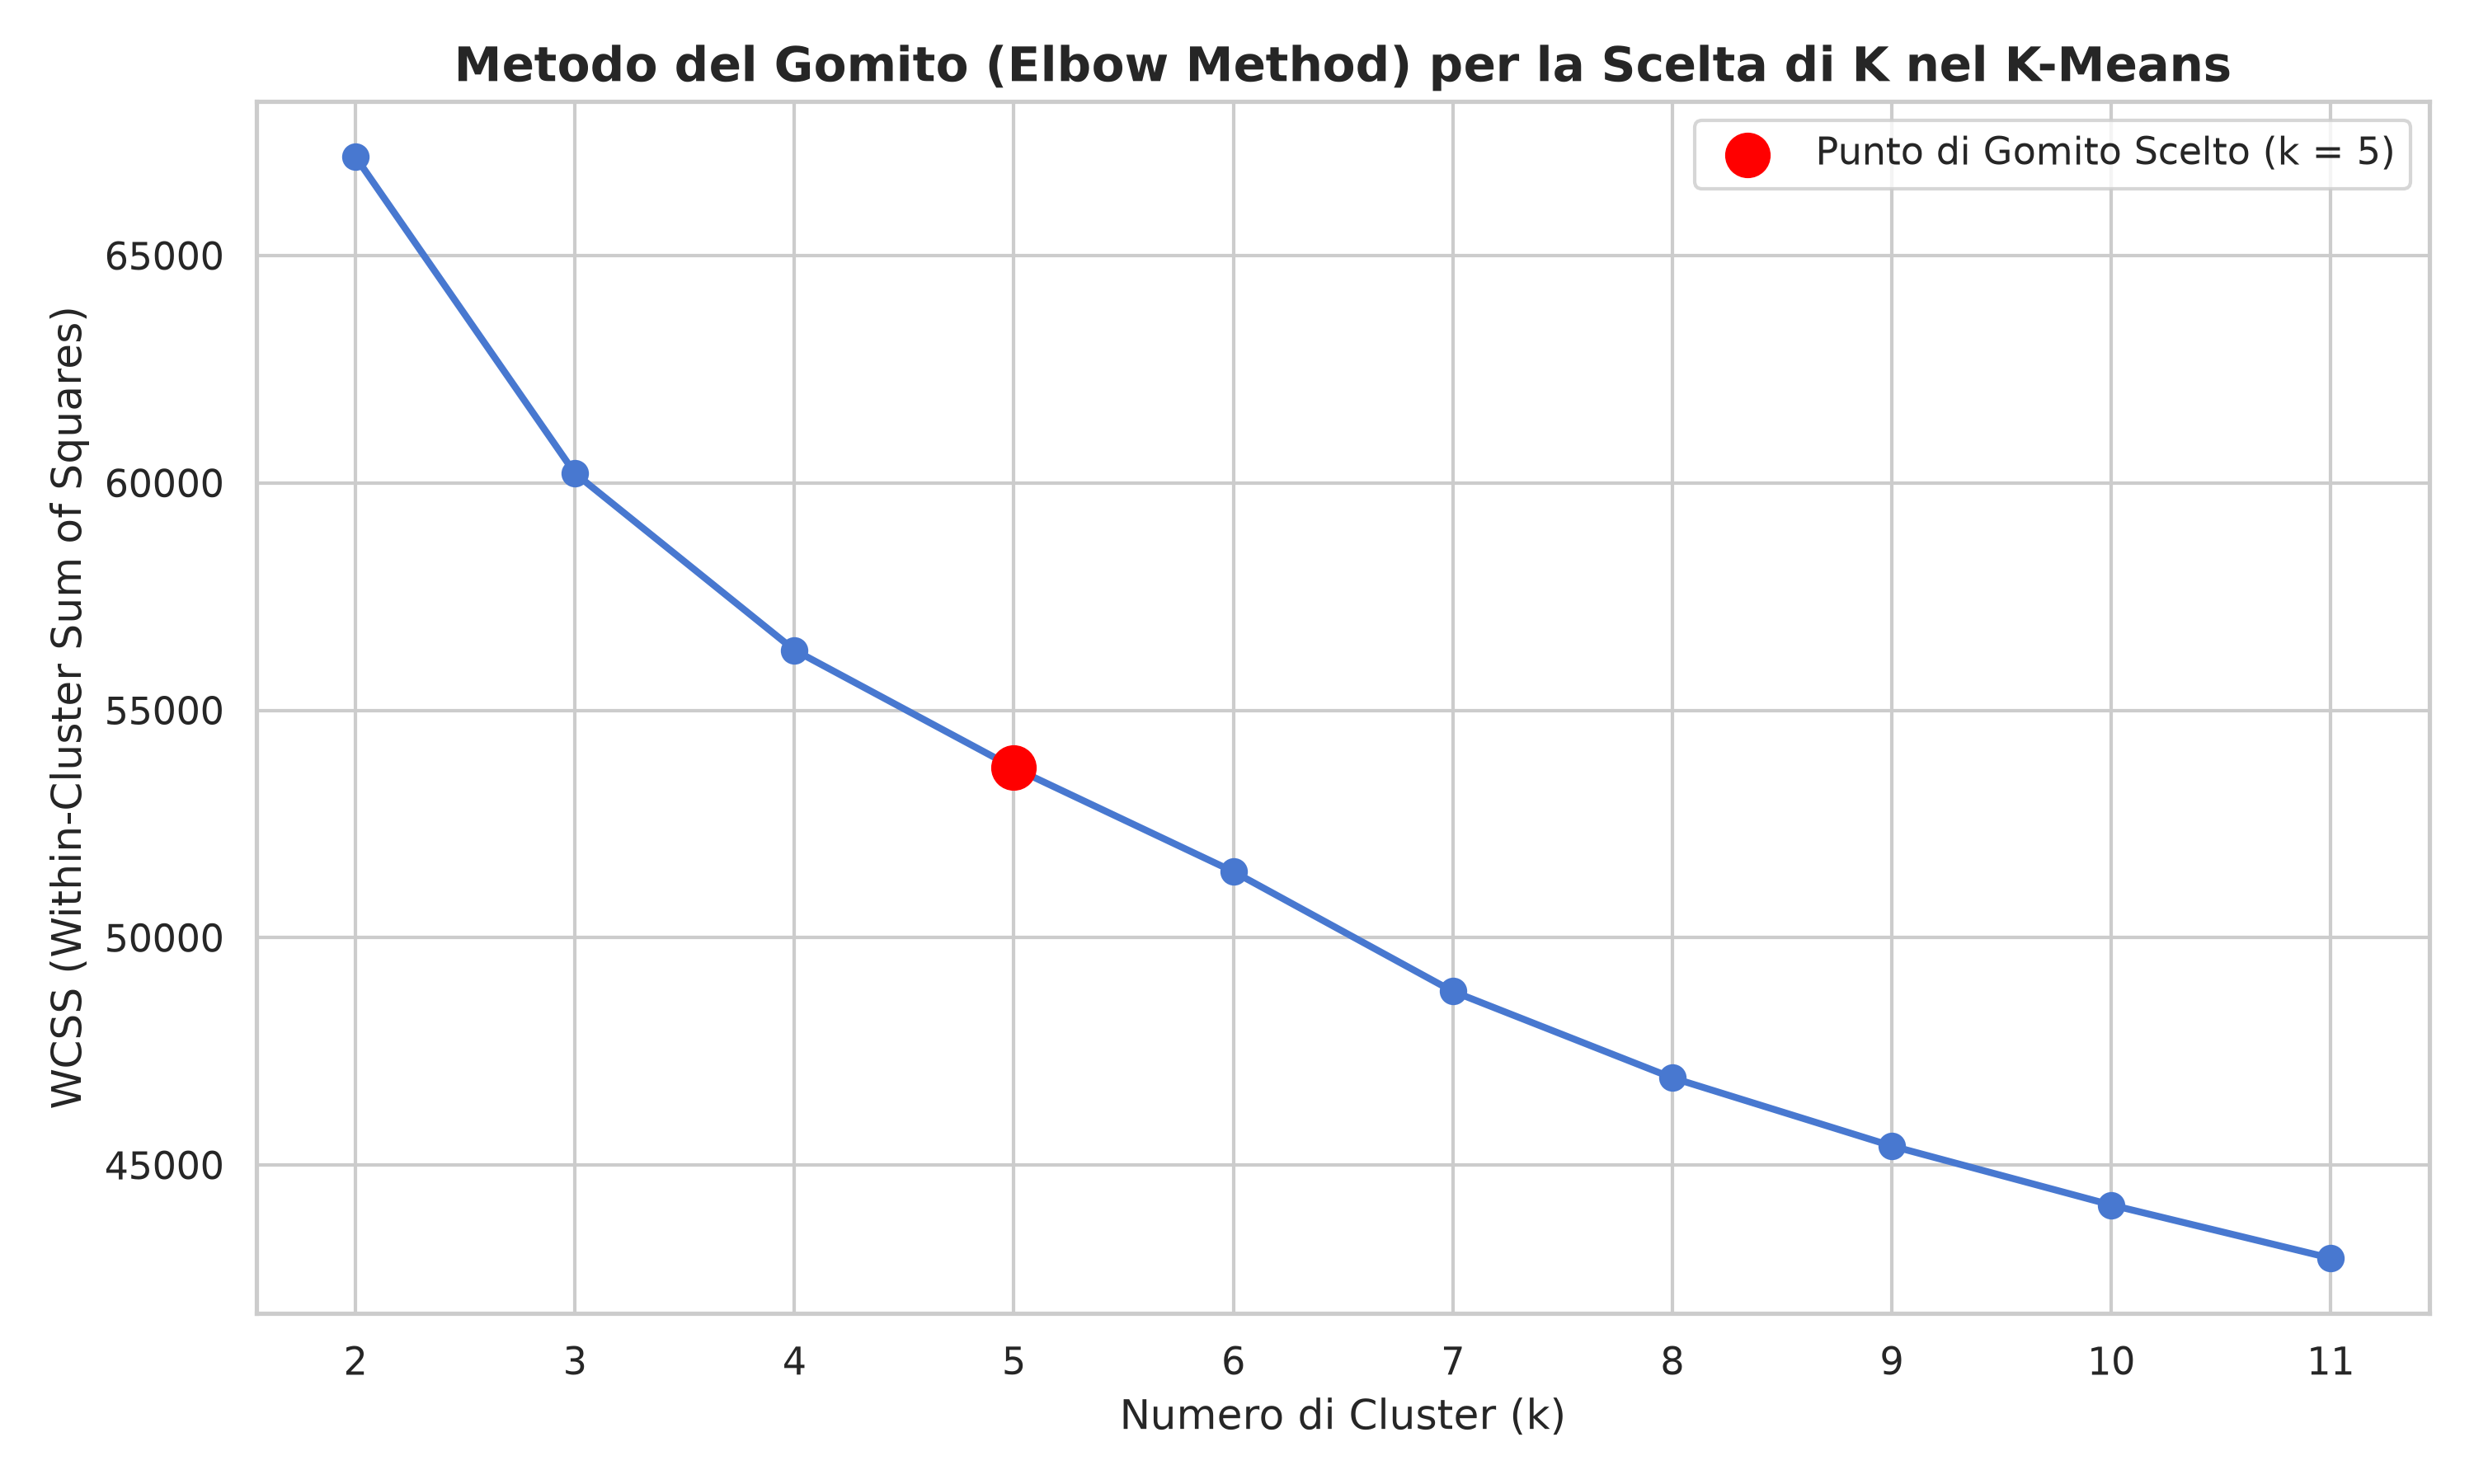
\includegraphics[width=0.75\textwidth]{figures/fig16_kmeans_elbow_wcss.png}
    \caption{Metodo del Gomito (Elbow Method) per la selezione di $k$ nel K-Means.}
    \label{fig:kmeans_elbow}
\end{figure}

\subsubsection{Analisi dei risultati ottenuti e Profiling dei Cluster}
Il modello K-Means con $k=5$ è stato proiettato sullo spazio 2D t-SNE (Figura \ref{fig:kmeans_tsne}). In Figura \ref{fig:kmeans_profiling} viene riportato il profiling acustico calcolando la media delle feature per ciascun cluster, consentendo di associare matematicamente ogni gruppo a uno specifico profilo d'ascolto (\textit{Mood Playlist}):
\begin{itemize}
    \item \textbf{Cluster 0 — High-Energy Electronic / Party:} Elevatissima loudness ed energy, speechiness minima e forte componente strumentale (\textit{Techno, Trance}).
    \item \textbf{Cluster 1 — Urban \& Rap:} Massimi valori di speechiness e ballabilità (\textit{Hip-Hop, Rap}).
    \item \textbf{Cluster 2 — Melodic Pop \& R\&B:} Caratterizzato da massima valenza emotiva (positività) e sonorità armoniche.
    \item \textbf{Cluster 3 — High-Velocity / Workout:} Velocità ritmica estrema (\texttt{tempo} medio $>165$ BPM) e ritmica incessante (\textit{DnB, Hardstyle}).
    \item \textbf{Cluster 4 — Atmospheric \& Dark:} Bassa loudness, atmosfera introspettiva e tonalità cupe (\textit{Dark Trap, Emo, Ambient}).
\end{itemize}

\begin{figure}[H]
    \centering
    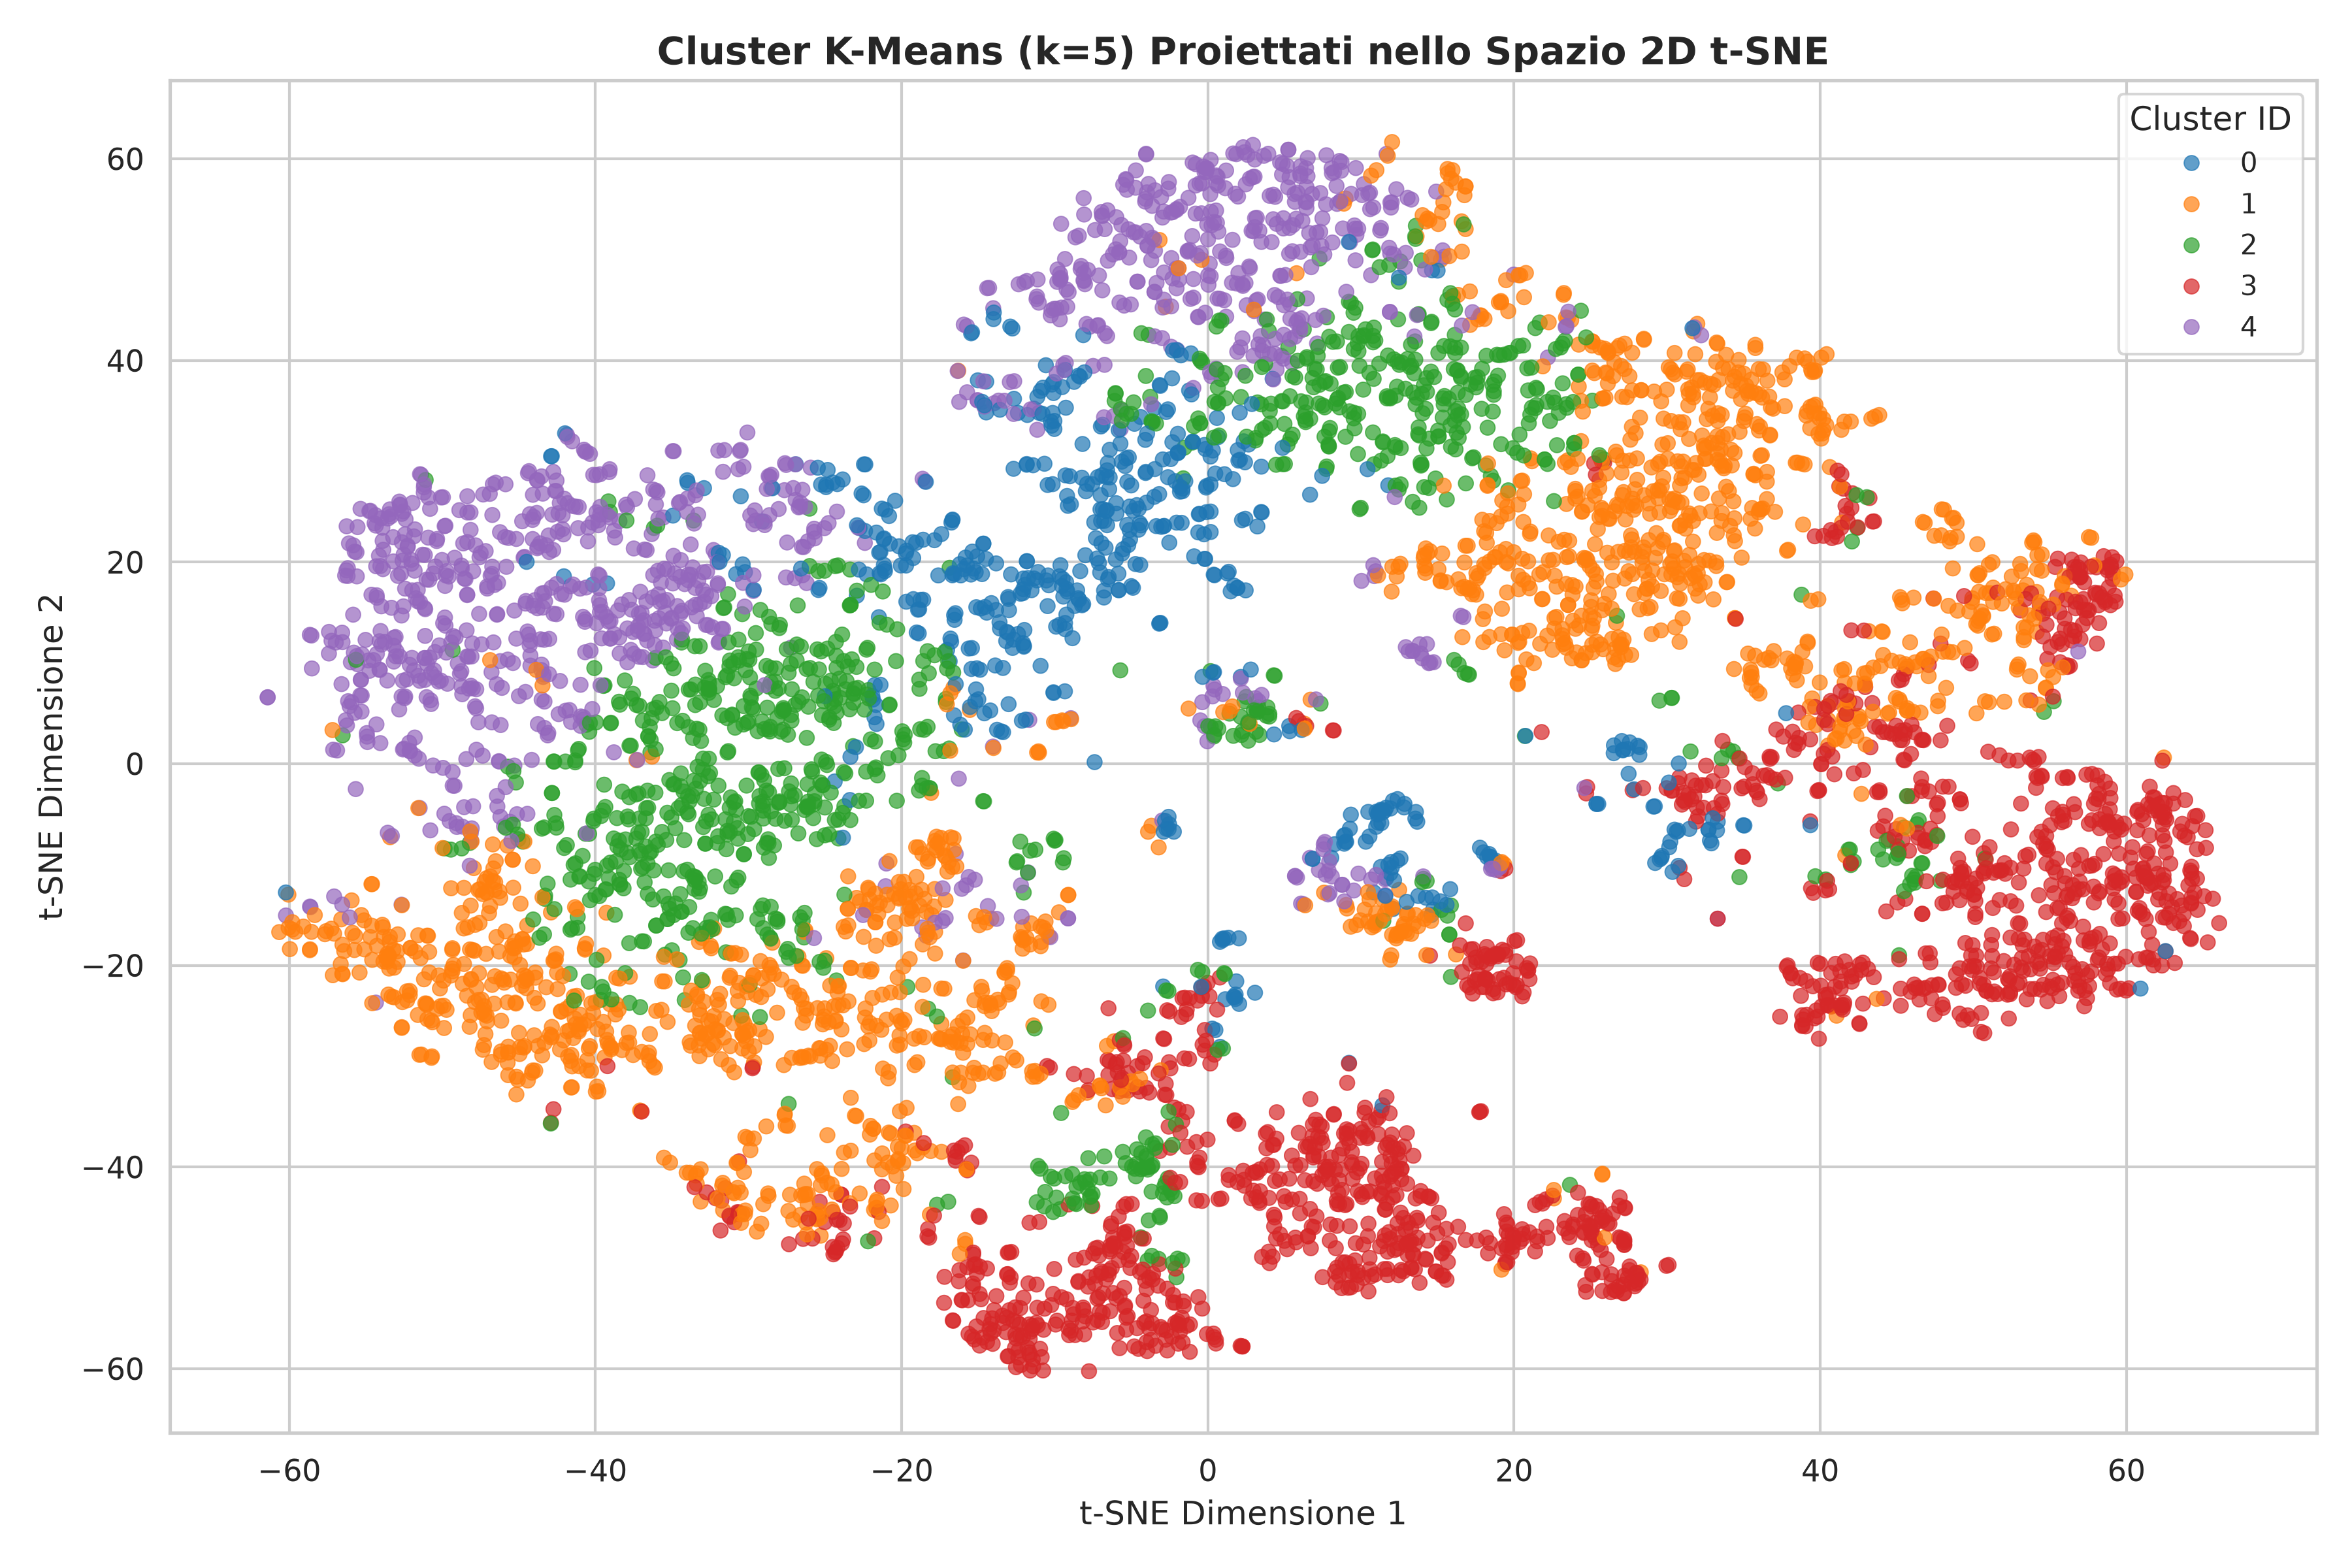
\includegraphics[width=0.88\textwidth]{figures/fig17_kmeans_tsne_clusters.png}
    \caption{Cluster K-Means ($k=5$) visualizzati sulla proiezione t-SNE 2D.}
    \label{fig:kmeans_tsne}
\end{figure}

\begin{figure}[H]
    \centering
    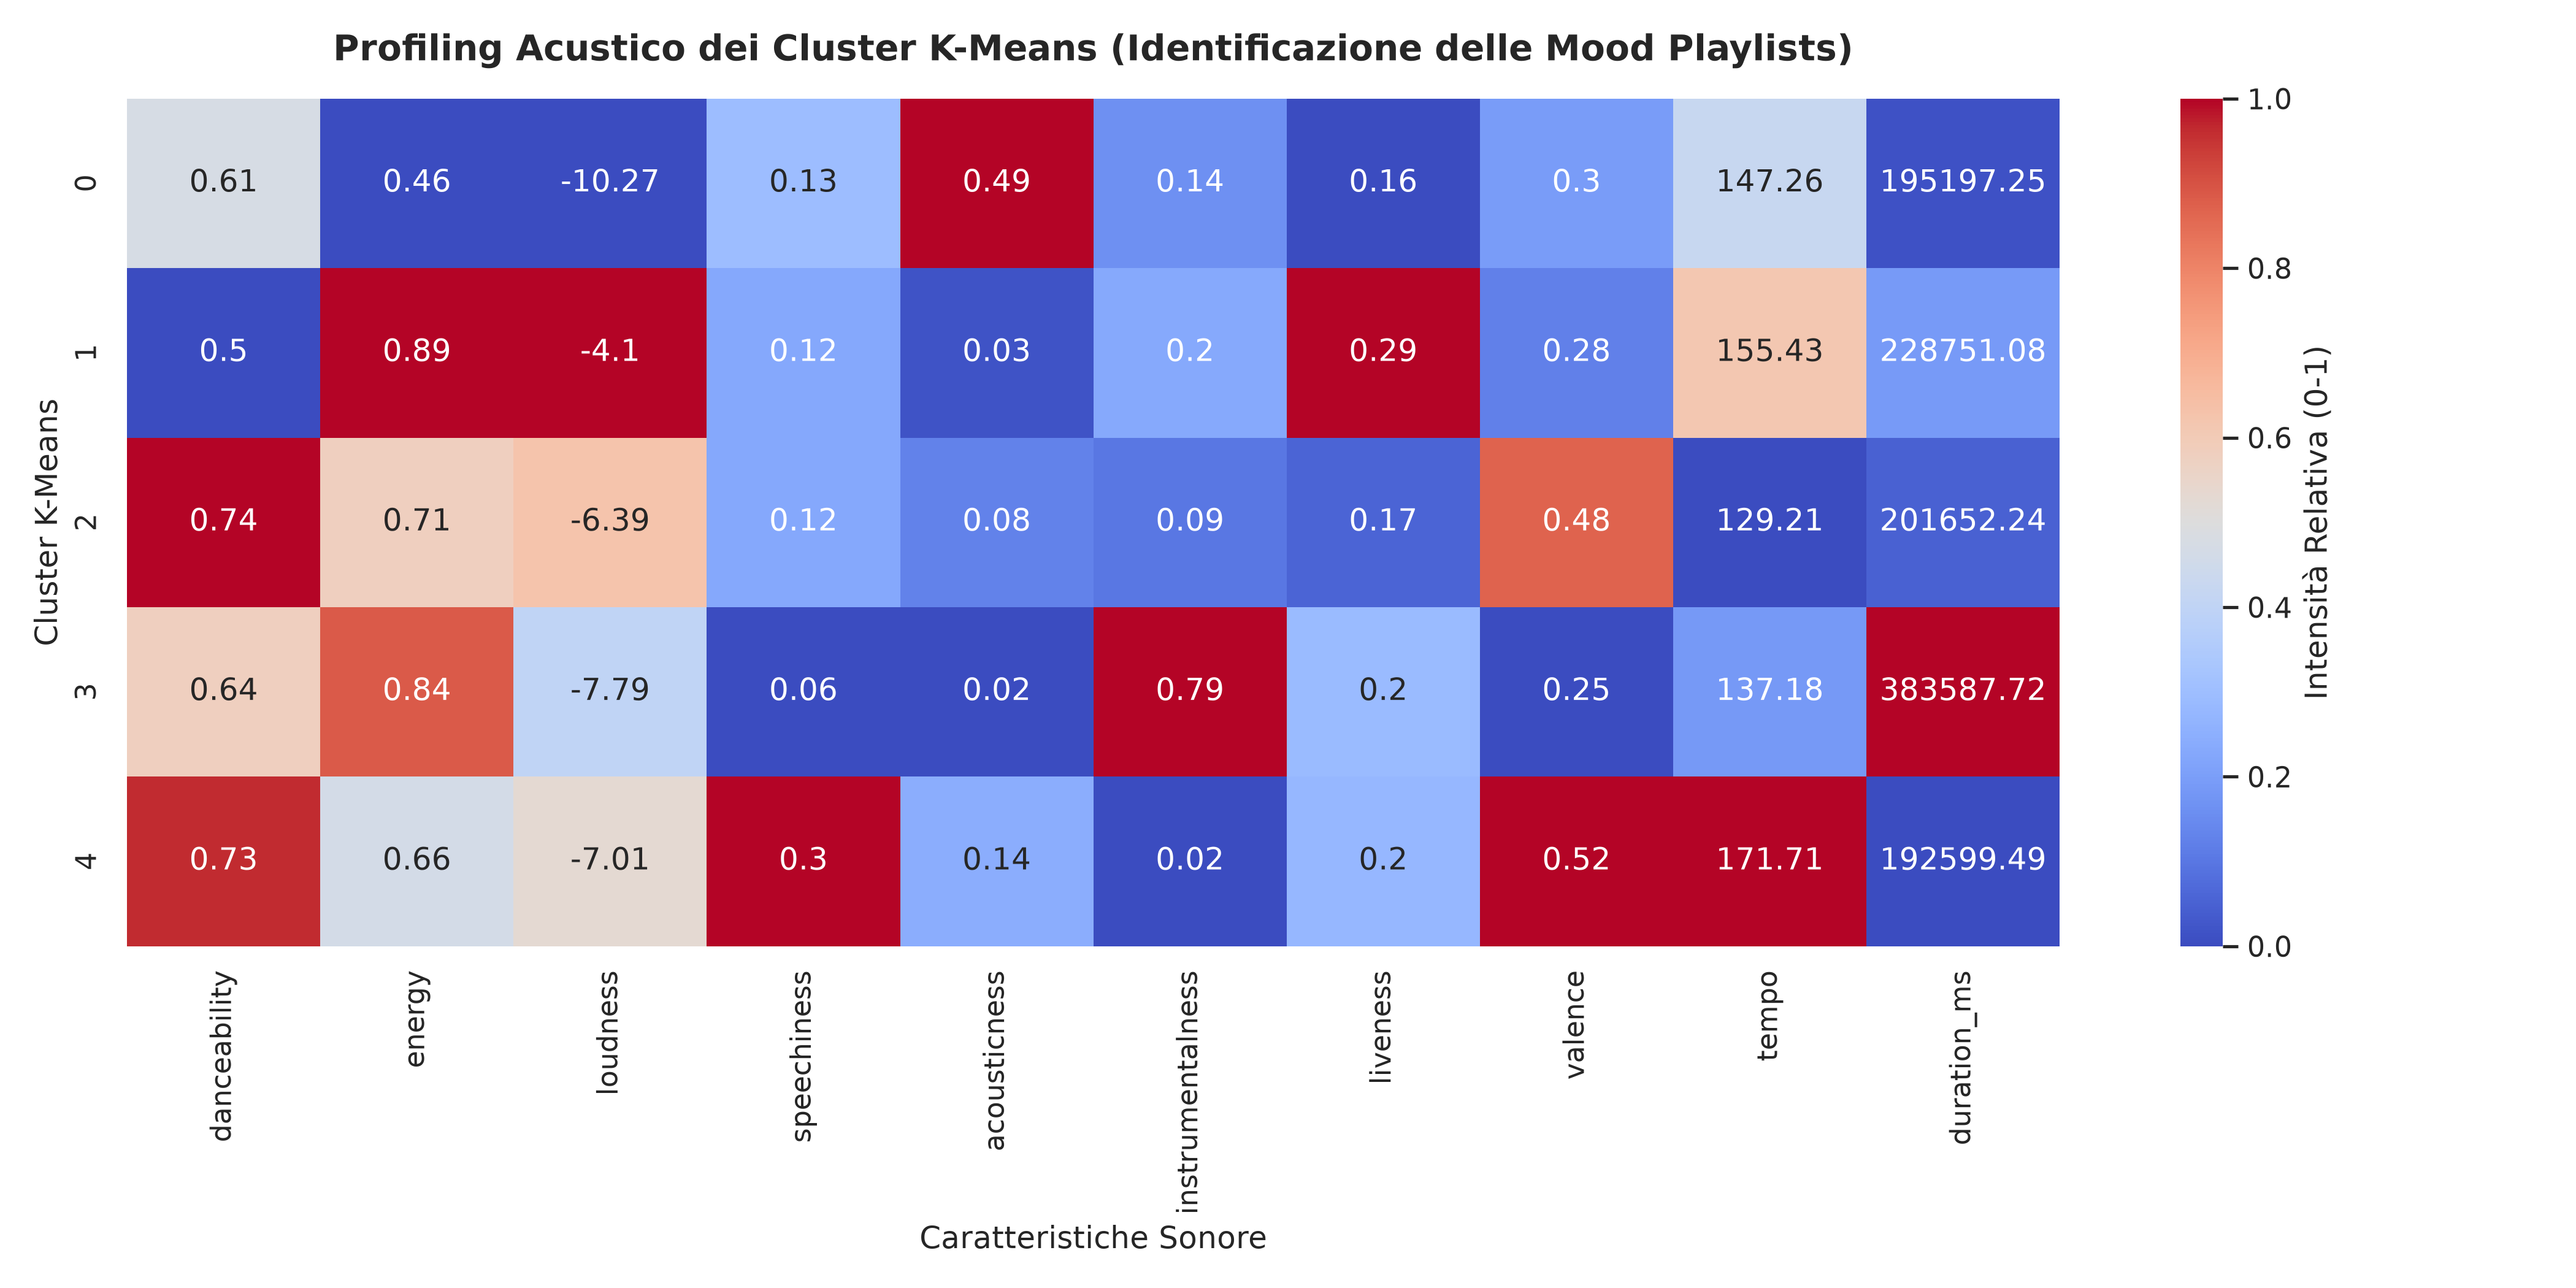
\includegraphics[width=0.92\textwidth]{figures/fig18_kmeans_feature_profiling.png}
    \caption{Profiling acustico dei cluster K-Means per l'identificazione automatica dei Mood.}
    \label{fig:kmeans_profiling}
\end{figure}

\subsubsection{Grafico della Silhouette per K-Means}
La qualità e la separazione dei cluster sono state valutate mediante il coefficiente di Silhouette\footnote{La Silhouette misura quanto un punto sia simile agli elementi del proprio cluster rispetto a quelli dei cluster contigui, assumendo valori tra -1 e +1.}. La Figura \ref{fig:kmeans_silhouette} mostra profili di ampiezza uniformi e una quota trascurabile di valori negativi, attestando che la partizione in 5 macro-mood rispetta la topologia dello spazio audio.

\begin{figure}[H]
    \centering
    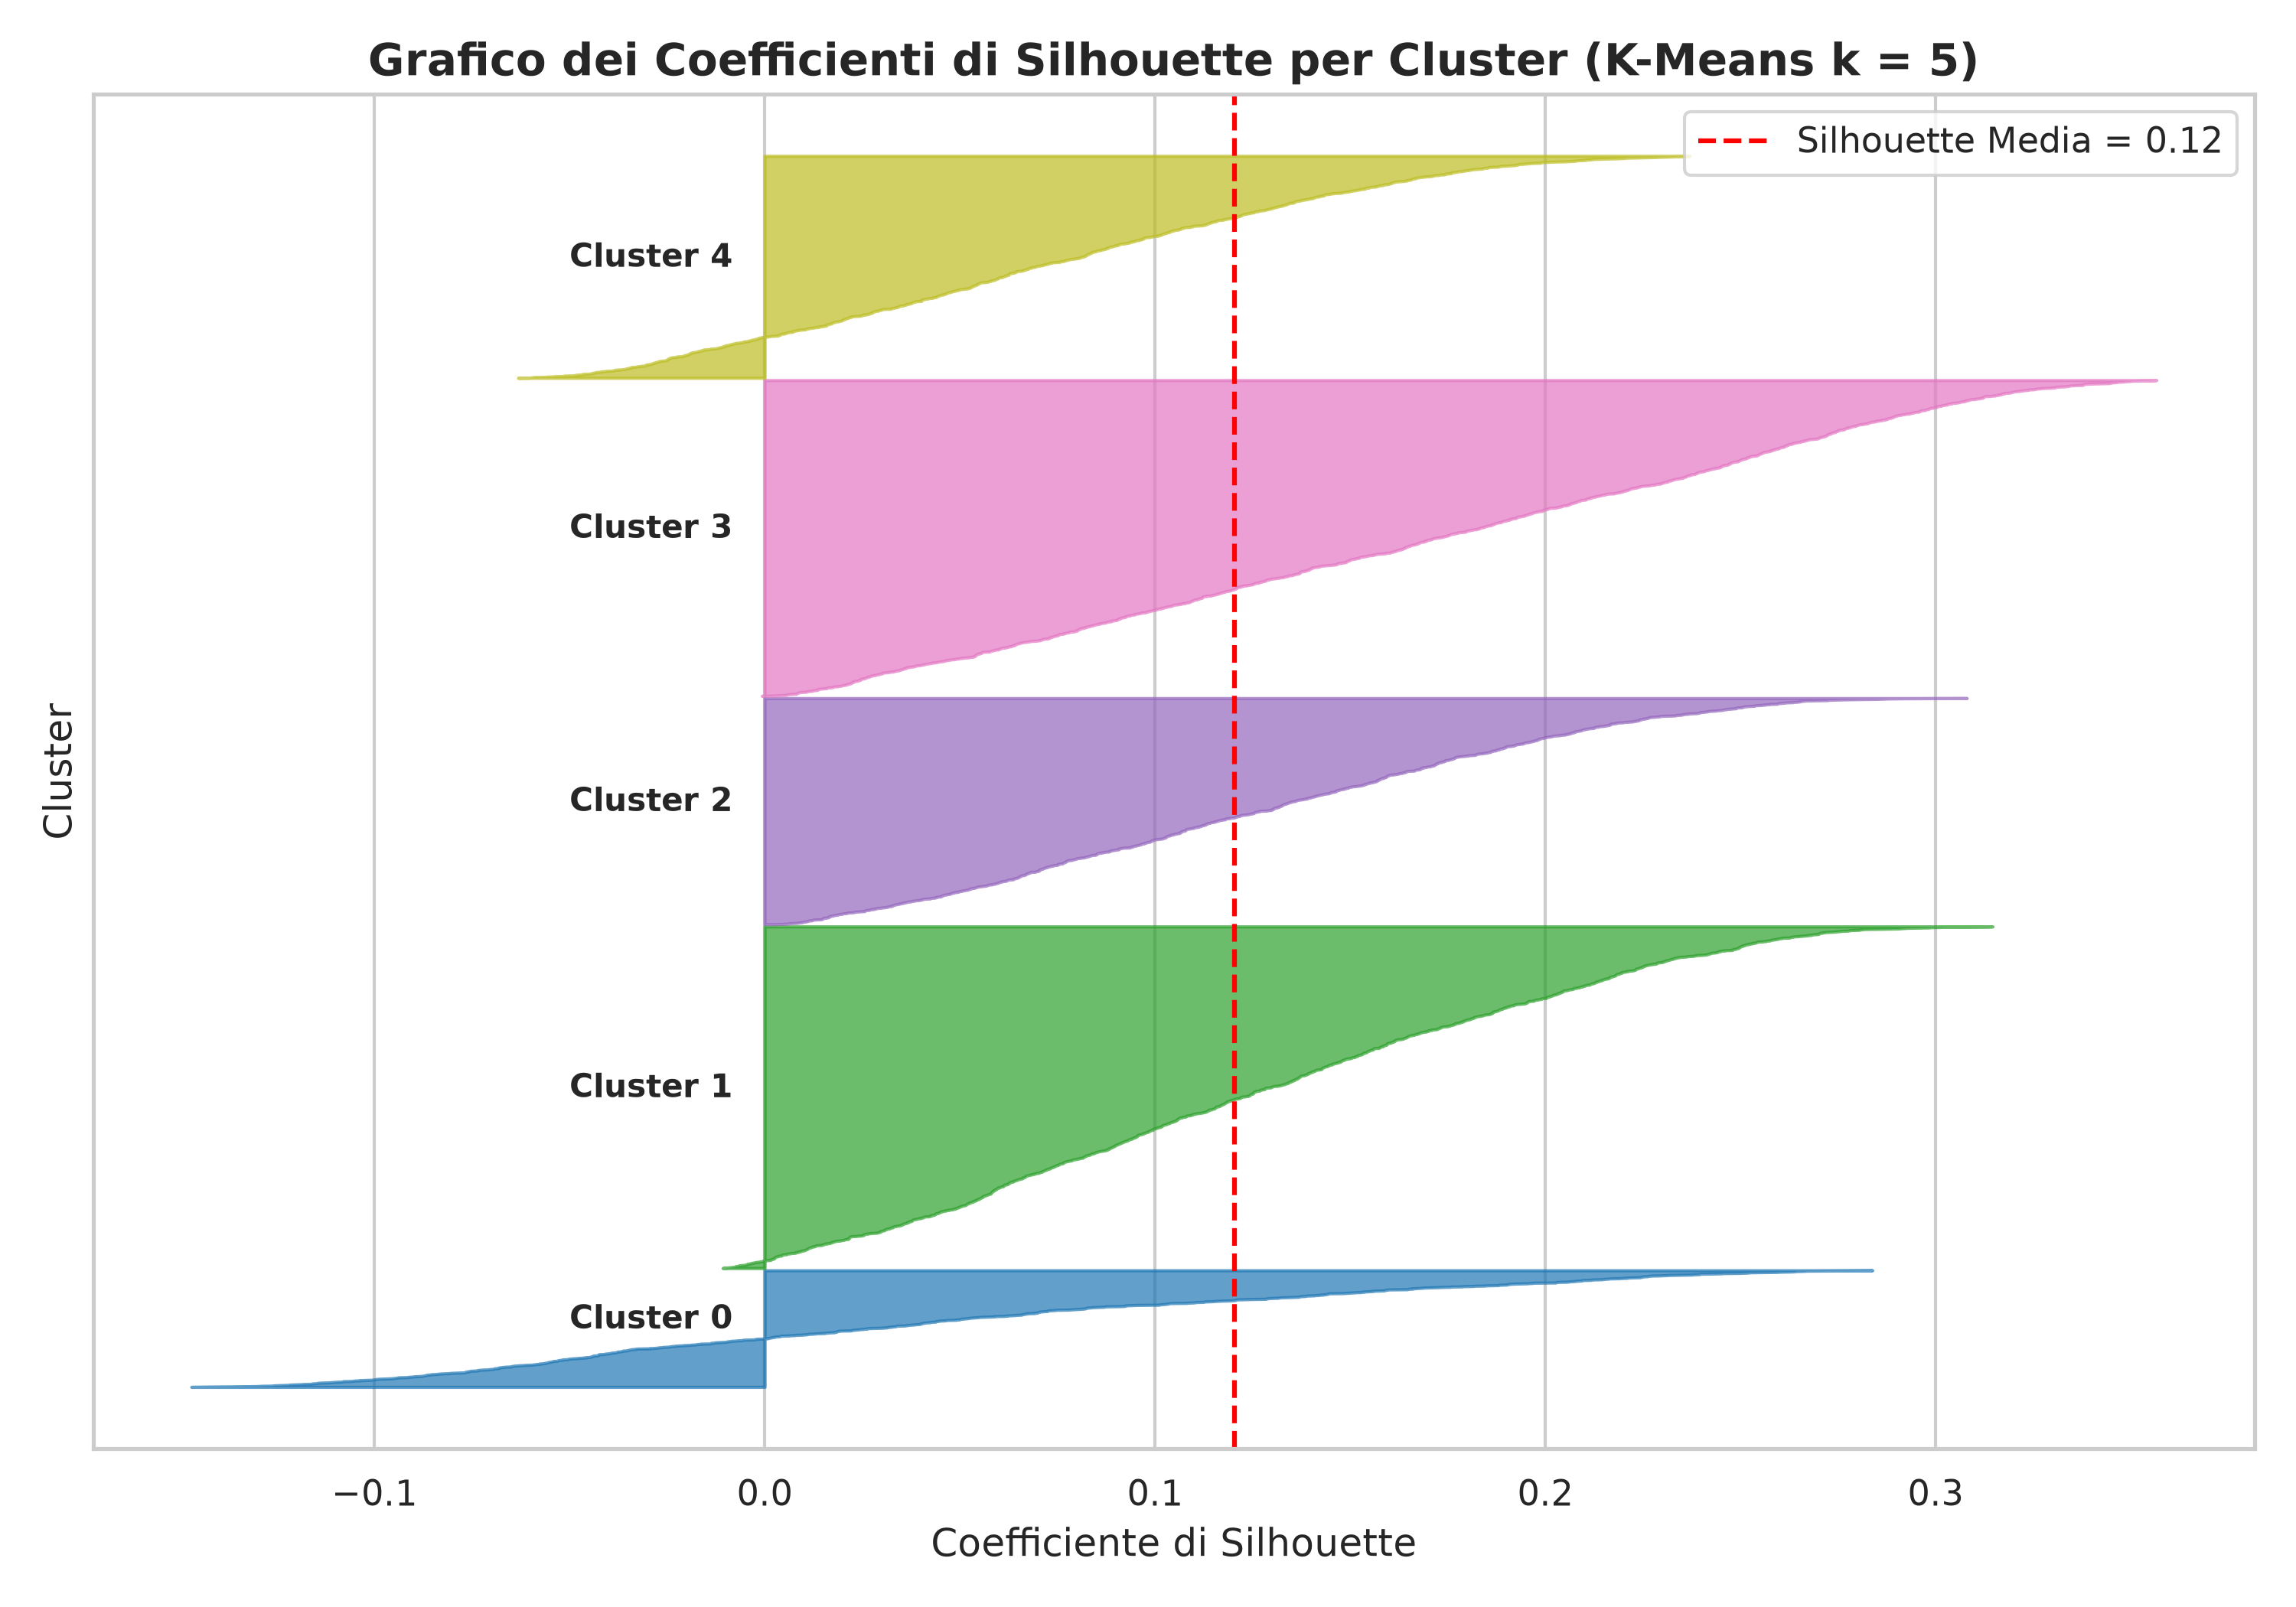
\includegraphics[width=0.75\textwidth]{figures/fig19_kmeans_silhouette_plot.png}
    \caption{Grafico della Silhouette per il modello K-Means ($k=5$).}
    \label{fig:kmeans_silhouette}
\end{figure}

\subsection{DBSCAN}
DBSCAN (\textit{Density-Based Spatial Clustering of Applications with Noise}) identifica i cluster come regioni dense nello spazio dati separate da aree a bassa densità, senza imporre forme geometriche predefinite ed etichettando automaticamente i punti isolati come rumore (\texttt{label} = -1).

\subsubsection{Applicazione dell'algoritmo DBSCAN}
Per determinare il raggio $\epsilon$, è stato impiegato il metodo dei $k$-Nearest Neighbors, graficando la distanza tra ciascun punto e il suo 5° vicino più prossimo ($k = \text{min\_samples} = 5$). In Figura \ref{fig:dbscan_knn} la curva evidenzia un netto ginocchio in corrispondenza di $\epsilon = 2.2$.
È stata inoltre esplorata una griglia parametrica $(\epsilon \times \text{min\_samples})$, riportata in Figura \ref{fig:dbscan_grid}. La combinazione $\epsilon = 2.2, \text{min\_samples} = 5$ identifica \textbf{8 cluster densi} e isola una frazione controllata di rumore pari al \textbf{6.9\%} (415 tracce).

\begin{figure}[H]
    \centering
    \begin{subfigure}[b]{0.49\textwidth}
        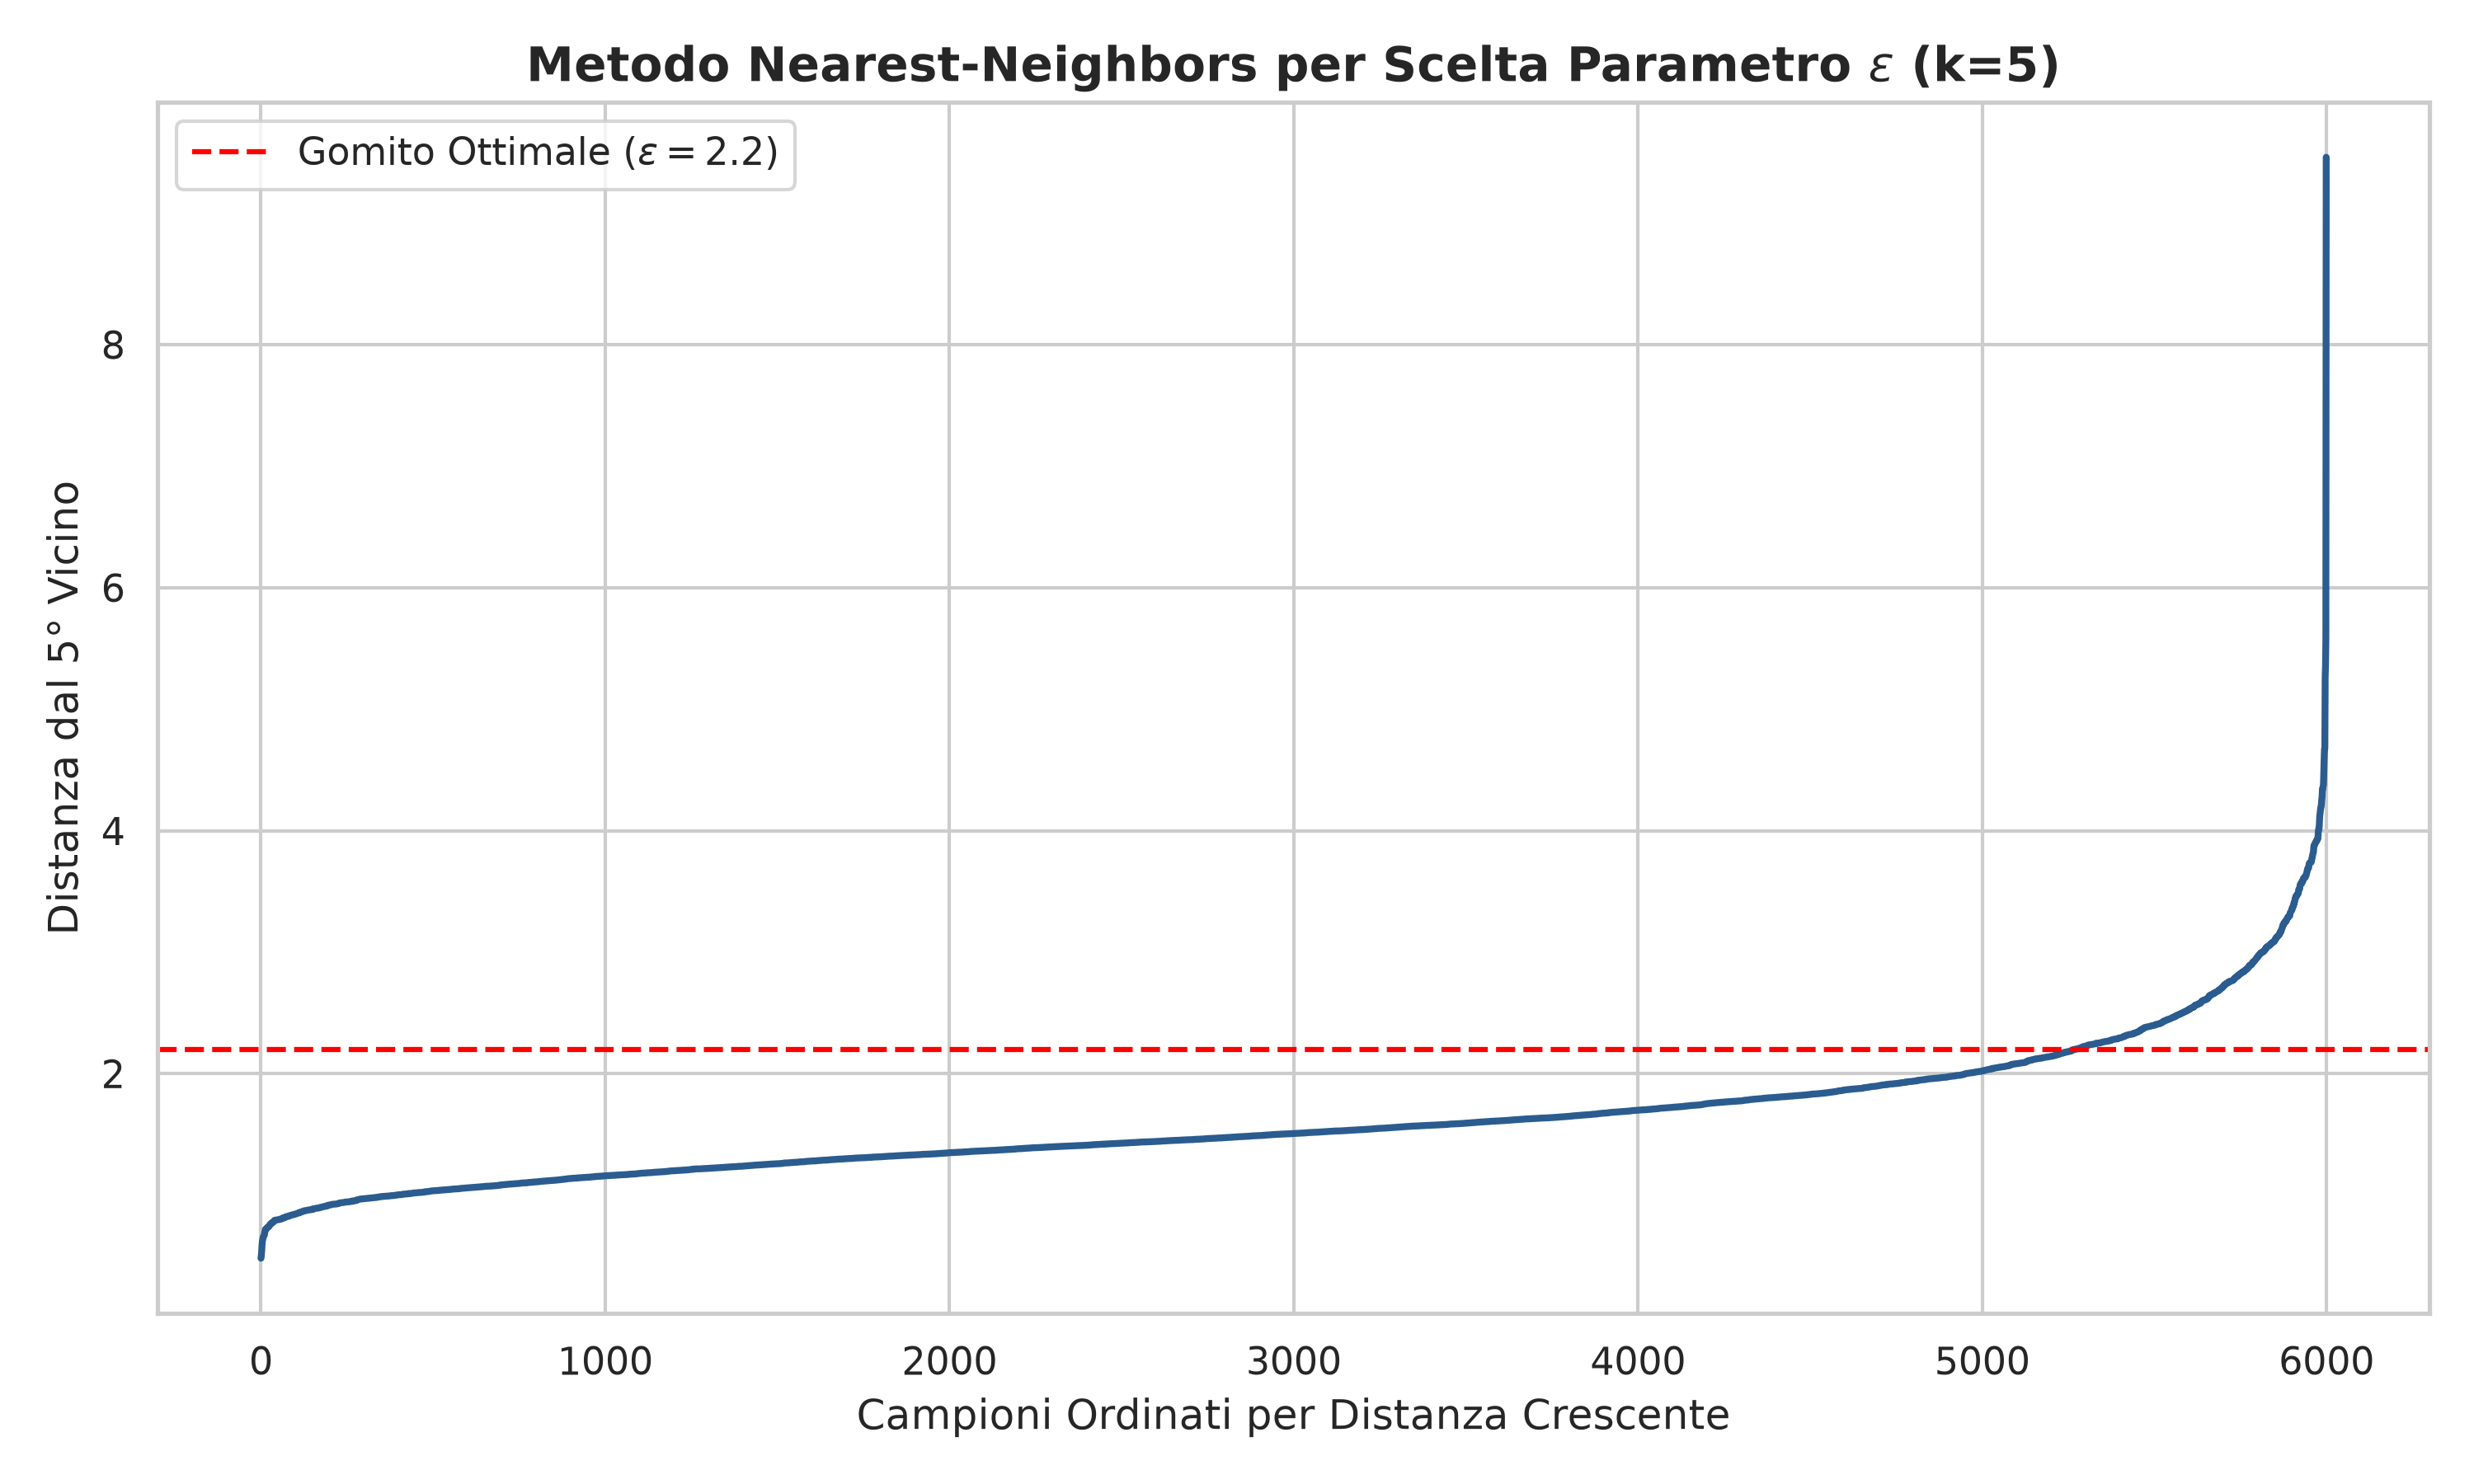
\includegraphics[width=\textwidth]{figures/fig20_dbscan_knn_distance.png}
        \caption{Grafico $k$-NN distance per la scelta di $\epsilon$.}
        \label{fig:dbscan_knn}
    \end{subfigure}
    \hfill
    \begin{subfigure}[b]{0.49\textwidth}
        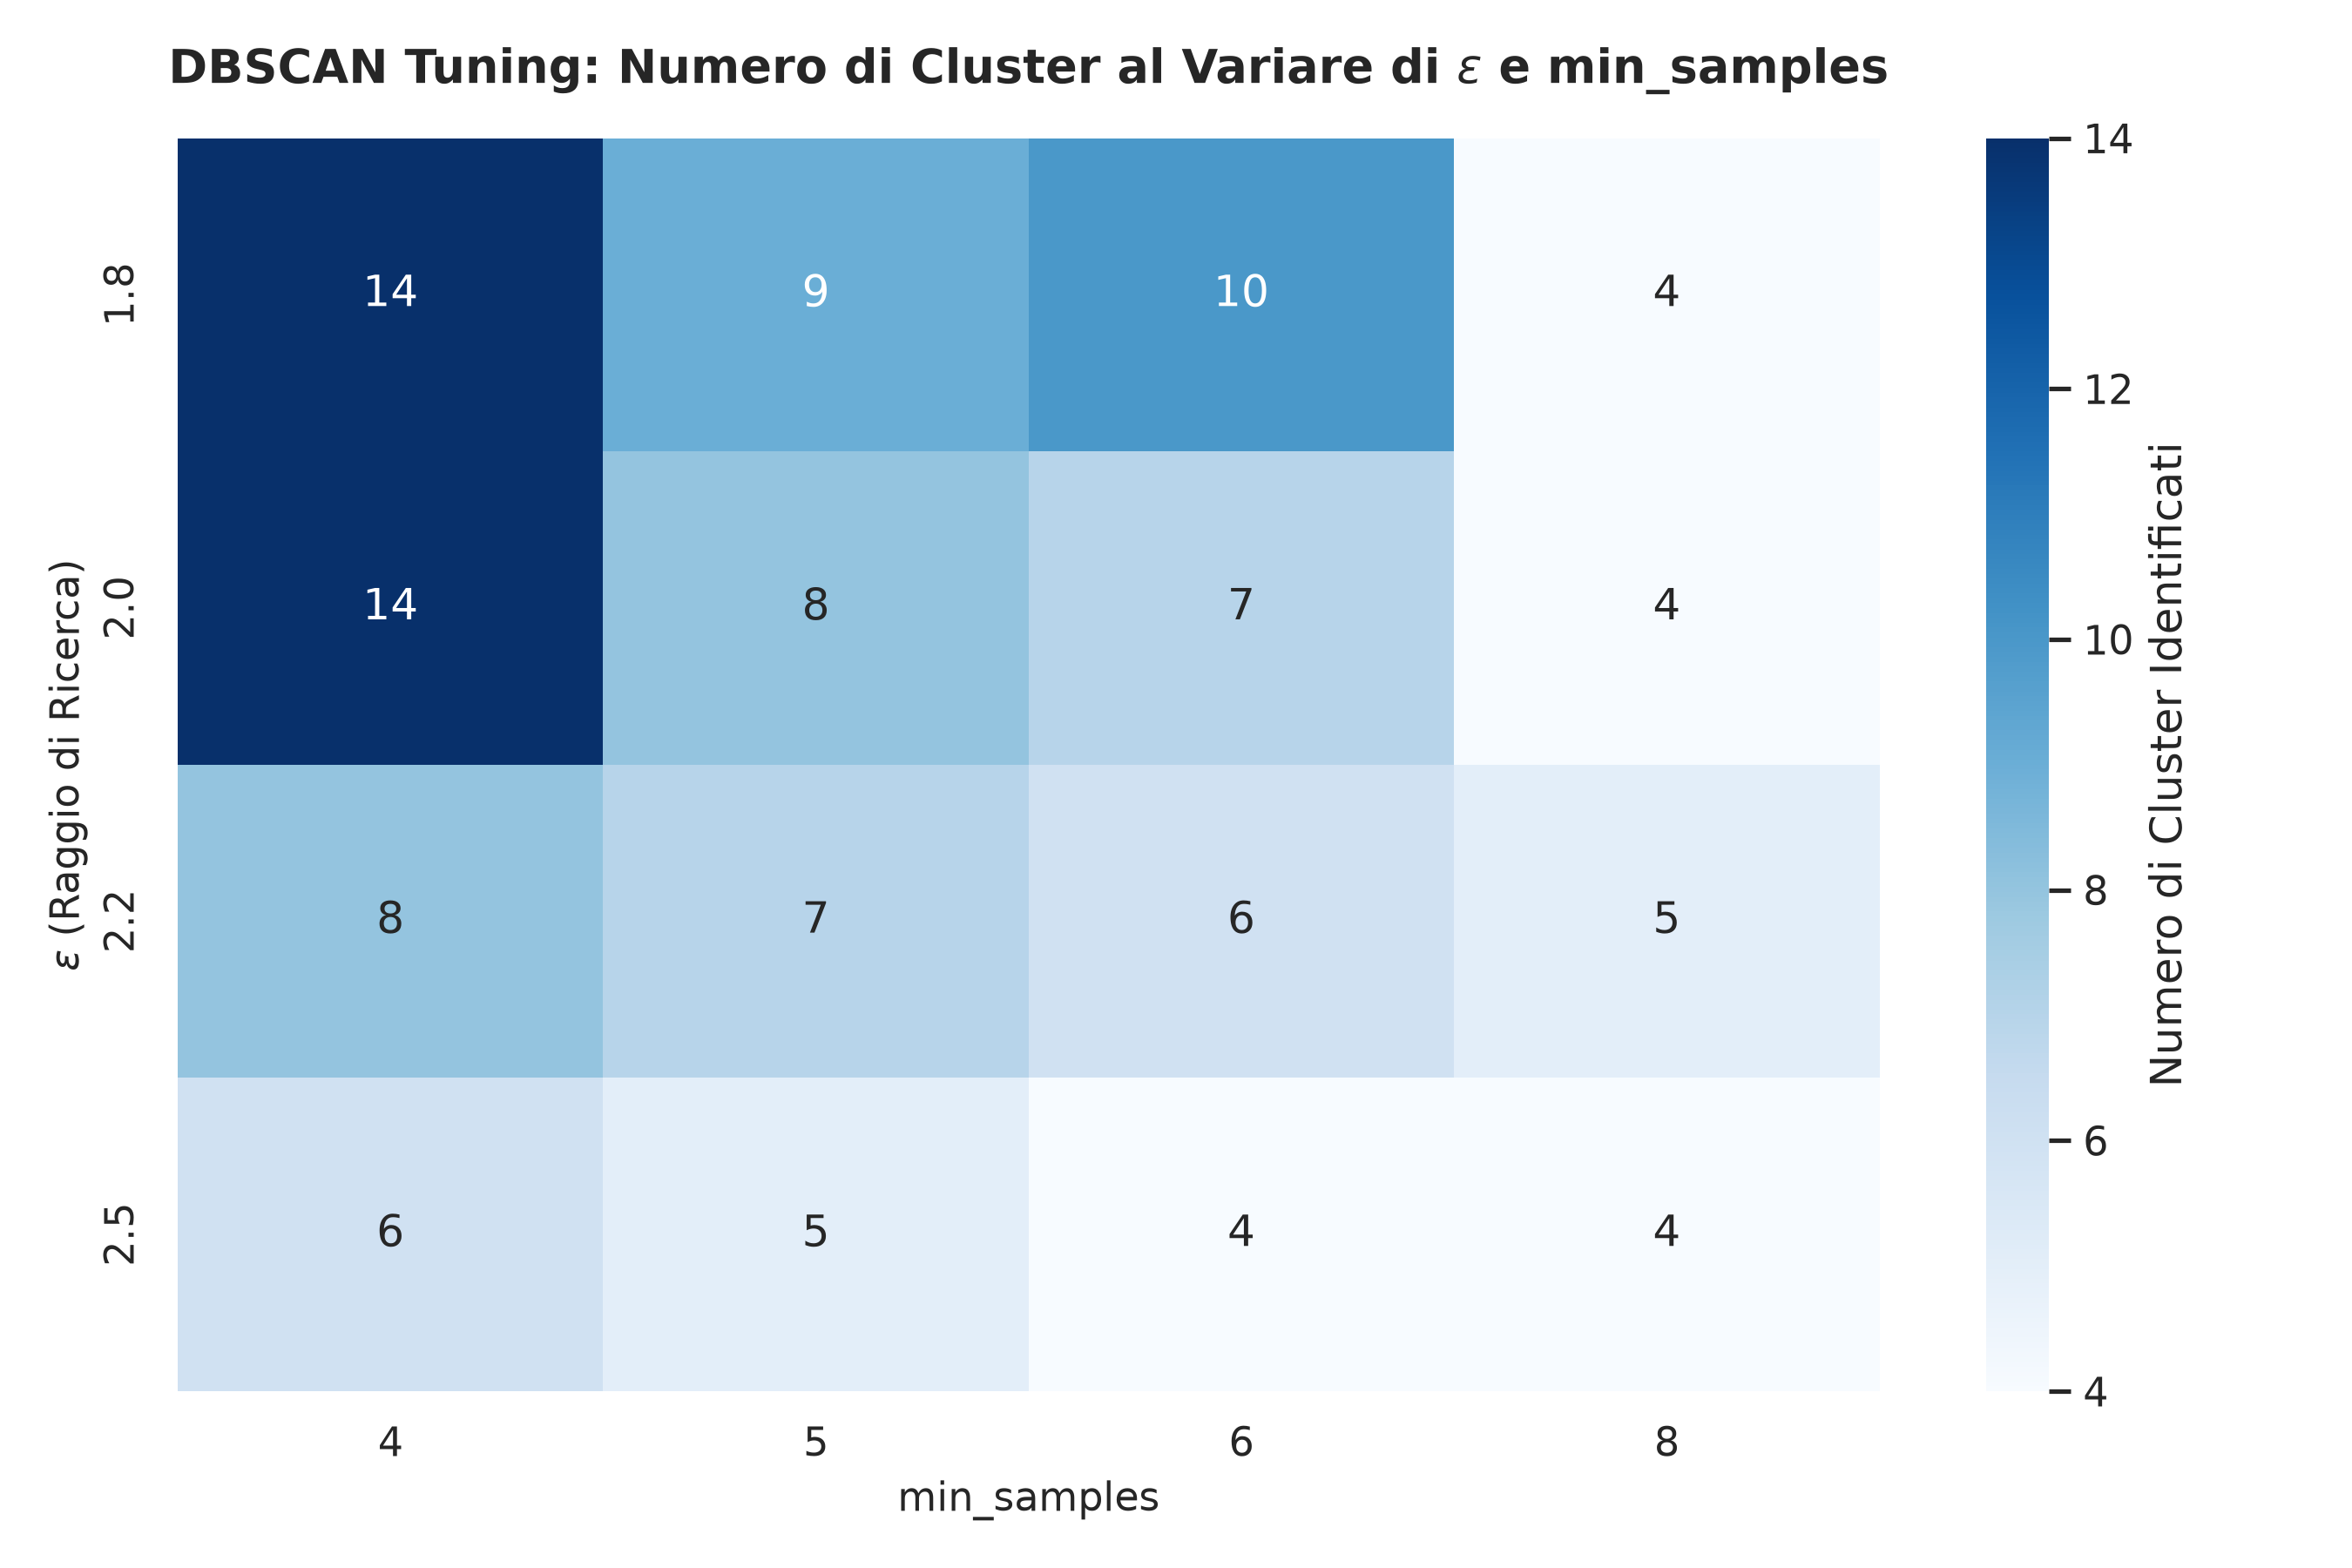
\includegraphics[width=\textwidth]{figures/fig21_dbscan_grid_search.png}
        \caption{Griglia di tuning parametri $(\epsilon \times \text{min\_samples})$.}
        \label{fig:dbscan_grid}
    \end{subfigure}
    \caption{Fase di tuning e calibrazione dei parametri per l'algoritmo DBSCAN.}
\end{figure}

\subsubsection{Analisi dei risultati ottenuti e Diagnostica del Rumore}
In Figura \ref{fig:dbscan_tsne} sono illustrati gli 8 cluster DBSCAN insieme ai punti di rumore (evidenziati con marker a croce rossa).
I boxplot in Figura \ref{fig:dbscan_noise} indagano il motivo per cui tali brani sono stati respinti come rumore:
\begin{itemize}
    \item \textbf{Durata anomala (\texttt{duration\_ms}):} Molti brani rumorosi hanno durate anomale superiori a 7-10 minuti o intro inferiori a 30 secondi.
    \item \textbf{Speechiness estrema:} Comprende tracce parlate, interviste, sketch e campionamenti non convenzionali.
    \item \textbf{BPM eccentrici:} Brani con velocità superiori a 210 BPM o fluttuazioni ritmiche atipiche.
\end{itemize}

\begin{figure}[H]
    \centering
    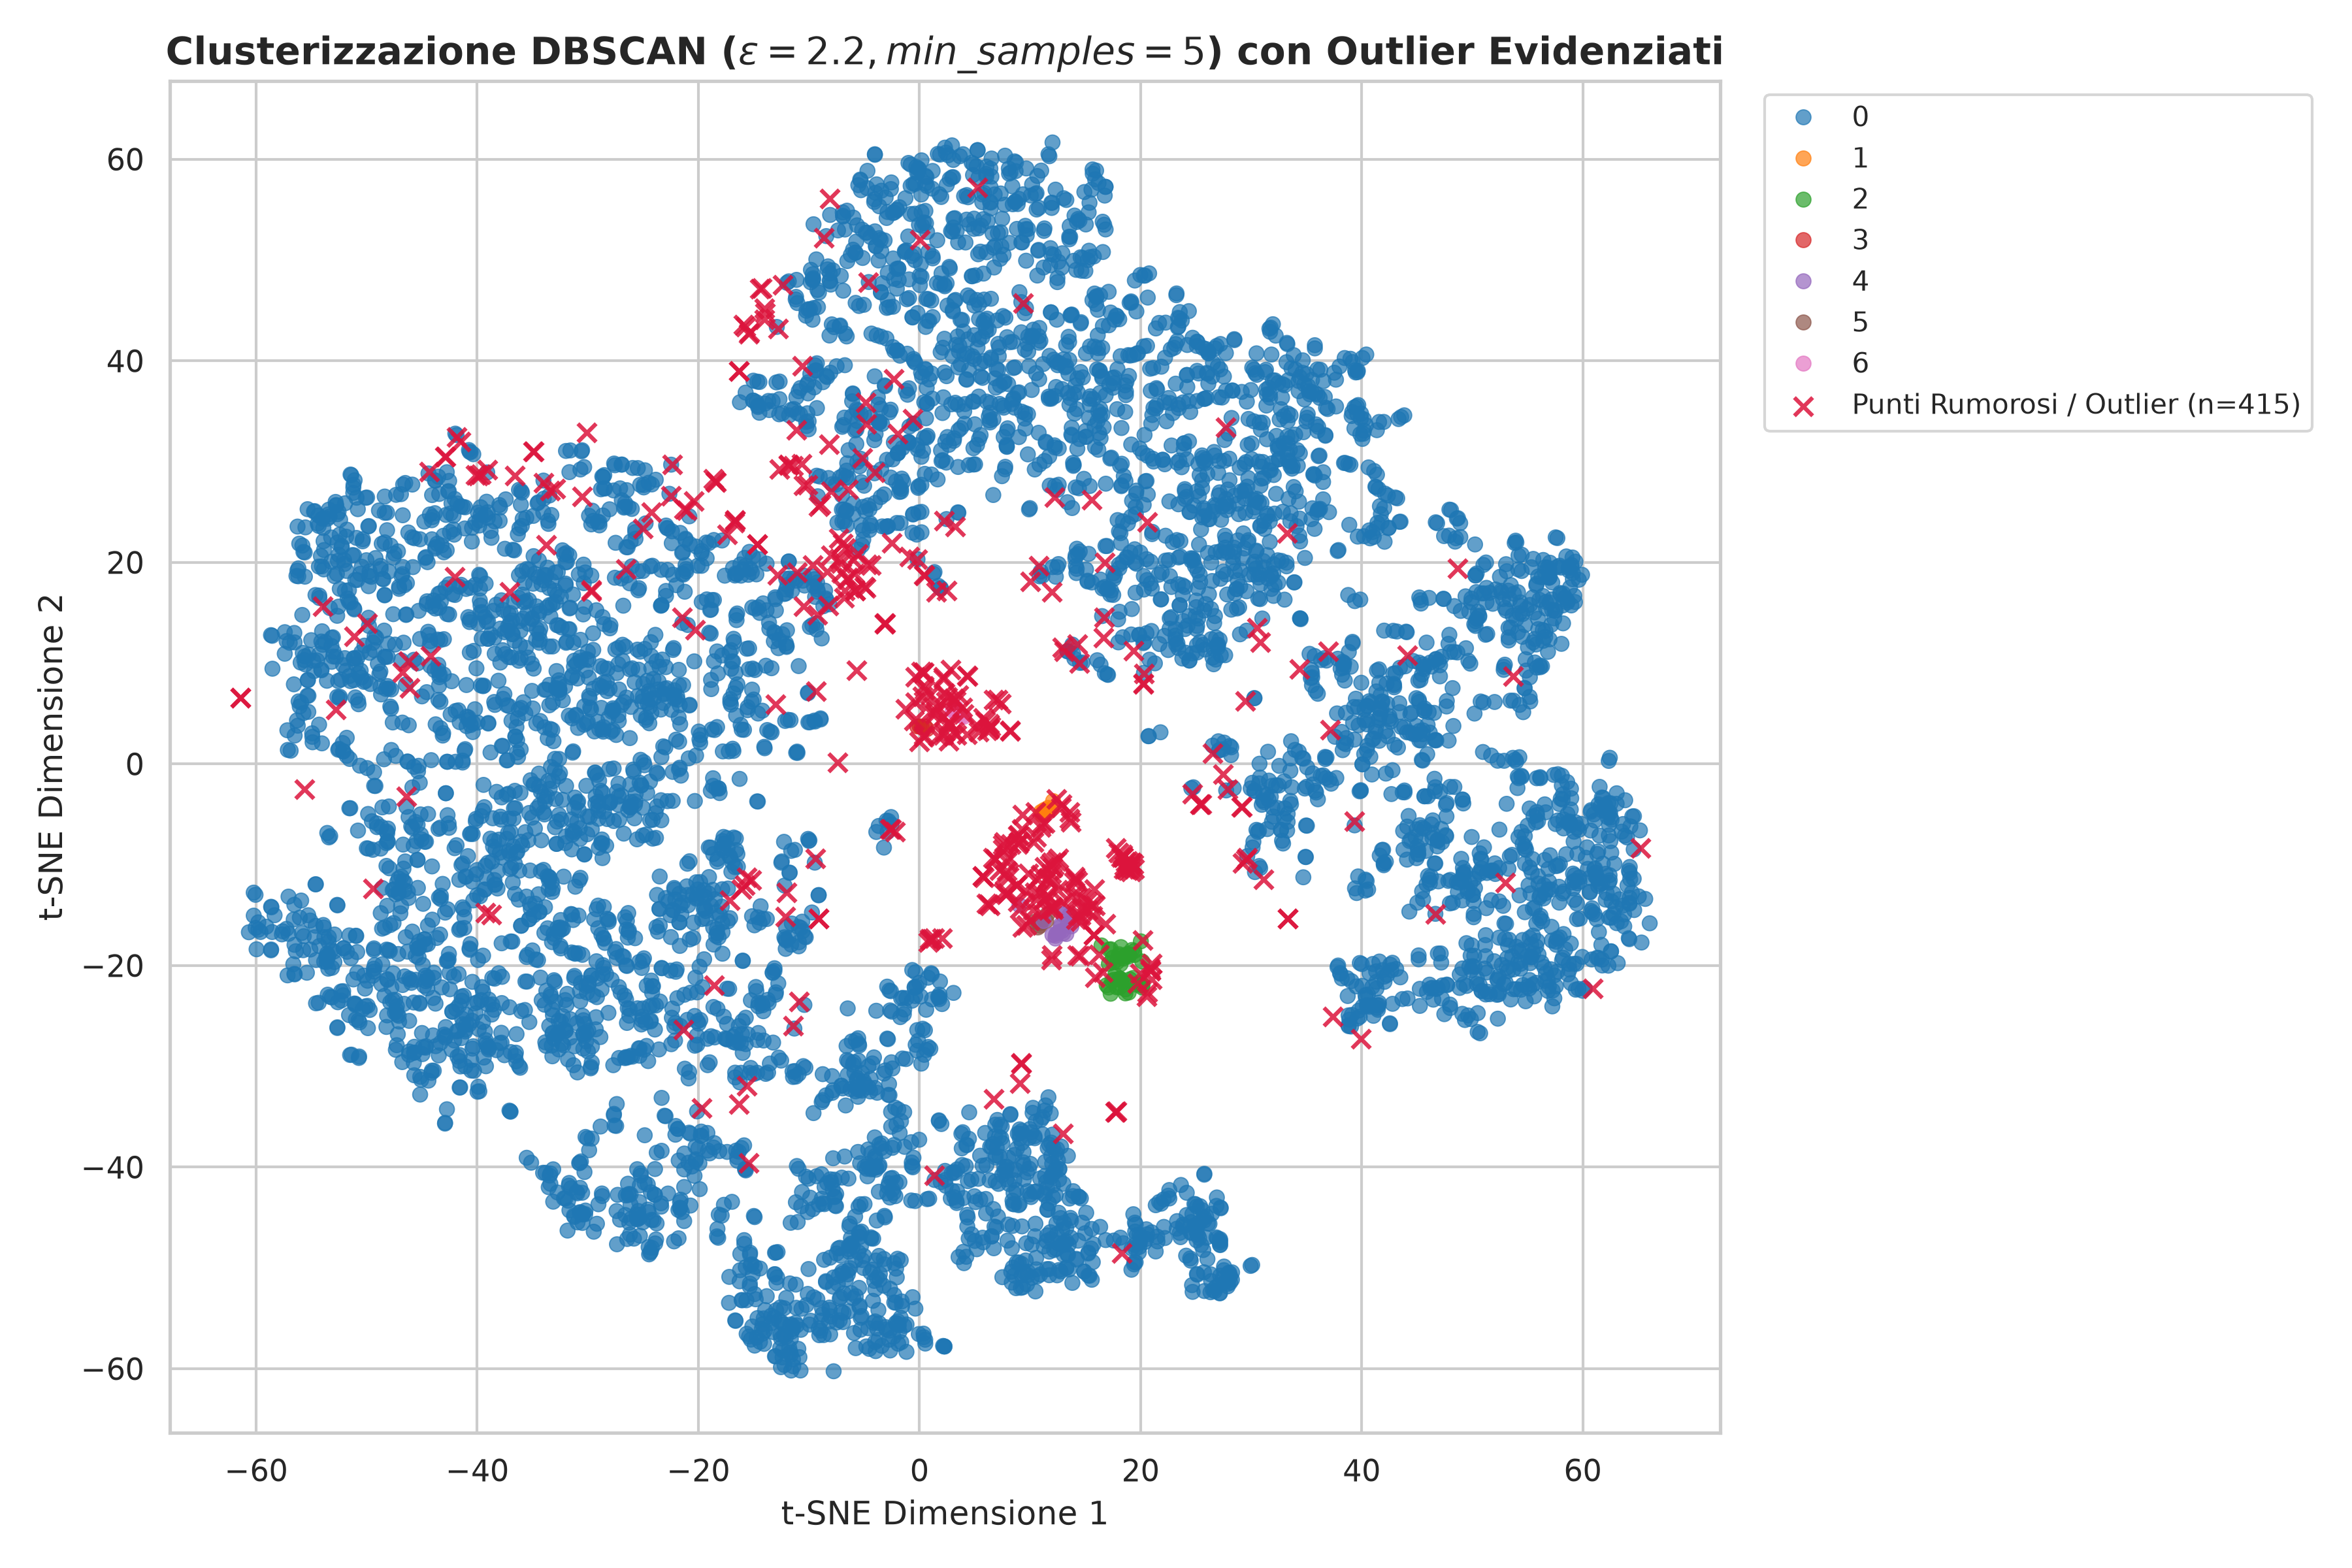
\includegraphics[width=0.88\textwidth]{figures/fig22_dbscan_tsne_clusters_noise.png}
    \caption{Cluster DBSCAN con isolamento ed evidenziazione dei punti di rumore / outlier.}
    \label{fig:dbscan_tsne}
\end{figure}

\begin{figure}[H]
    \centering
    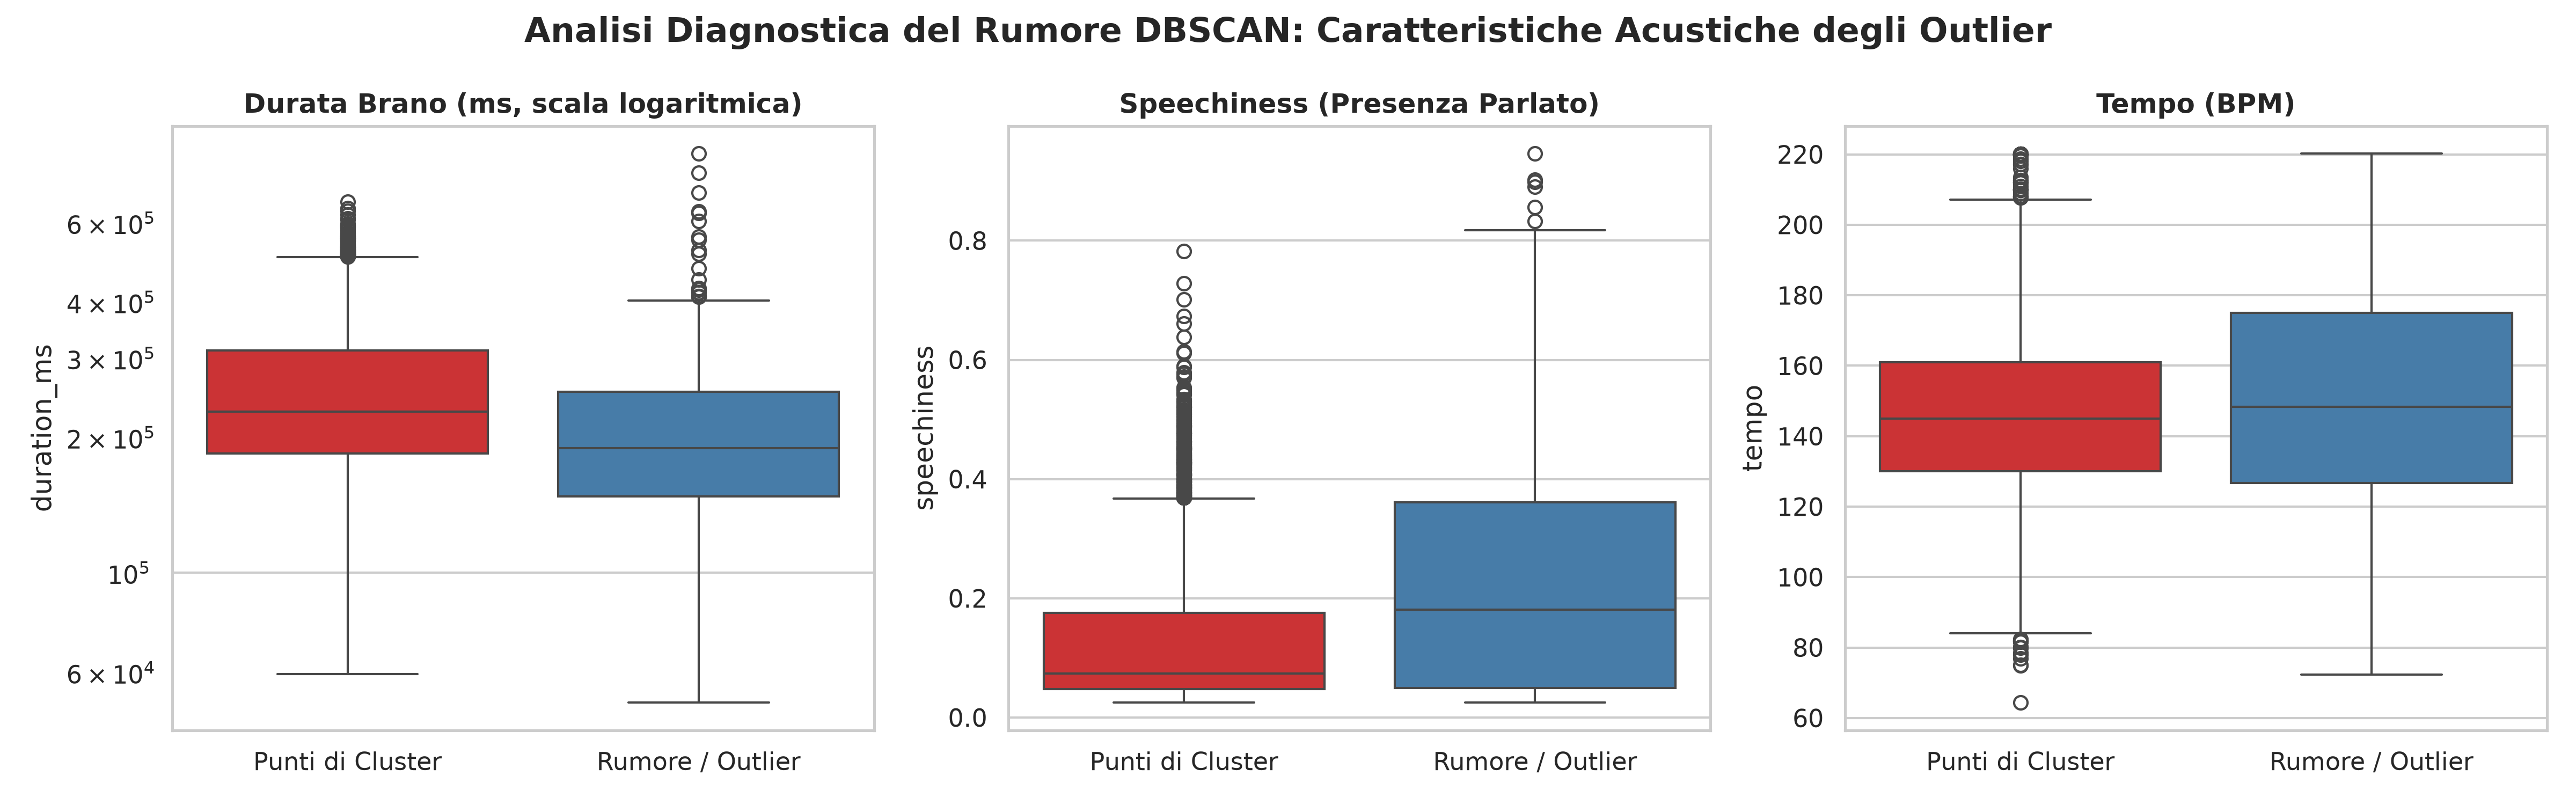
\includegraphics[width=0.95\textwidth]{figures/fig23_dbscan_noise_profiling.png}
    \caption{Analisi diagnostica del rumore DBSCAN: confronto delle distribuzioni su feature anomale.}
    \label{fig:dbscan_noise}
\end{figure}

\newpage
% =========================================================================
% CAPITOLO 5: BUSINESS CASE E CONCLUSIONI
% =========================================================================
\section{Business Case finale e Conclusioni}

L'analisi congiunta condotta attraverso modelli supervisionati e non supervisionati fornisce soluzioni concrete per le sfide operative e strategiche dell'industria musicale contemporanea:

\begin{enumerate}
    \item \textbf{Motore di Raccomandazione per Mood (Clustering):} Le etichette di genere tradizionali risultano spesso rigide o fuorvianti: ad esempio brani etichettati come \textit{Pop} o \textit{Dark Trap} possono condividere gli stessi parametri ritmici ed emotivi. Il K-Means dimostra come raggruppare i brani in 5 macro-mood matematici, consentendo alle piattaforme di streaming di generare playlist dinamiche e contestualizzate (\textit{Workout, Focus, Party, Chillout}) basate unicamente sull'affinità sonora latente.
    \item \textbf{Filtro di Controllo Qualità e Anomaly Detection (DBSCAN):} La capacità di DBSCAN di isolare il 6.9\% di tracce come rumore fornisce uno strumento automatizzato di controllo qualità per i distributori digitali, intercettando file corrotti, podcast erroneamente catalogati come canzoni o registrazioni amatoriali con anomalie di volume e durata prima dell'inserimento nei cataloghi editoriali.
    \item \textbf{Valutazione Matematica dei Nuovi Brani (Classificazione):} Il modello finale di \textit{Stacking Classifier} (con un'accuratezza vicina al \textbf{69\% su 15 generi sbilanciati} e una \textbf{Macro-AUC di 0.94}) attesta che le sole metriche audio numeriche sono in grado di prevedere con notevole precisione il posizionamento commerciale di una traccia demo appena registrata, fornendo a direttori artistici ed etichette discografiche un solido indicatore quantitativo sul potenziale target di mercato prima di investire risorse promozionali.
\end{enumerate}

\end{document}
